% Define colors
\definecolor{keywordcolor}{RGB}{255,0,0}
\definecolor{Classcolor}{RGB}{90, 90, 90}
\definecolor{Funcolor}{RGB}{191, 64, 191}
\definecolor{Logiccolor}{RGB}{51, 179, 255}
\definecolor{commentcolor}{RGB}{0,128,0}
\definecolor{stringcolor}{RGB}{163,21,21}

% Language definition
\lstdefinelanguage{CS}{
    language=C,
    morekeywords=
        {using, public, private, class, yield, return, new, if, else, out, try, catch, for, while, throw, foreach, in, using},
    morekeywords=[2]
        {ARRaycastManager, ARPlaneManager, GameObject, InventoryController, Vector3, ARPlane, Ray, RaycastHit, GetComponent, MeshRenderer, Quaternion},
    morekeywords=[3]
        {Start, Update, Awake, DelayedStart, IsPointerOverPlane, GetCurrentPlaneUnderGaze, SetPlaneColor, PlaceObjectOnDesk, ScreenPointToRay, SetActive, Euler, SetInventoryObject, Raycast},
    morekeywords=[4]
        {+, -, /, *, !, =, 0, 1, 2, 3, 4, 5, 6, 7, 8, 9, null, true, false}, % Define symbols as keywords
    morecomment=[l]{//},
    morecomment=[s]{/*}{*/},
    morestring=[b]",
    sensitive=true
}

% Listings settings
\lstset{
    language=CS,
    basicstyle=\footnotesize\ttfamily,
    keywordstyle=\color{keywordcolor}\bfseries,
    keywordstyle=[2]\color{Classcolor},
    keywordstyle=[3]\color{Funcolor},
    keywordstyle=[4]\color{Logiccolor},
    commentstyle=\color{commentcolor},
    stringstyle=\color{stringcolor},
    showstringspaces=false,
    breaklines=true,
    frame=single,
    numbers=left,
    numberstyle=\tiny\color{gray},
    tabsize=4,
    captionpos=b
}

\chapter{Feinkonzept und Realisierung}

\section{Entwicklungsumgebungen}
\subsection{Visual Studio 2022}
Visual Studio 2022 ist eine integrierte Entwicklungsumgebung (IDE) von Microsoft, die speziell für die Entwicklung von
Softwareanwendungen, Webanwendungen und Desktop-Anwendungen konzipiert ist. Es handelt sich um eine umfangreiche
Entwicklungsumgebung, die von Entwicklern weltweit für eine breite Palette von Anwendungsfällen eingesetzt wird.

\subsection{Unity}
Der Unity-Editor, entwickelt von Unity Technologies, fungiert als umfassende integrierte Entwicklungsumgebung (IDE)
und zentrale Arbeitsumgebung für die Konzeption und Umsetzung von 2D-, 3D-, Augmented Reality (AR) und Virtual Reality
(VR) Anwendungen und Spielen. Als Kernelement der Unity-Plattform spielt der Editor eine entscheidende Rolle in der
Entwicklung von Projekten, die auf Unity-Technologien basieren.

Die Funktionalität des Unity-Editors erstreckt sich über verschiedene Aspekte der Softwareentwicklung, angefangen bei
der visuellen Gestaltung von Szenen und Spielwelten bis hin zur Implementierung komplexer Logik und Interaktionen. Die
folgenden Abschnitte vertiefen die Schlüsselmerkmale und Funktionen des Unity-Editors, die ihn zu einem essenziellen
Werkzeug für Entwickler machen.

\subsubsection{Multidisziplinäre Unterstützung und Integration}
Der Unity-Editor zeichnet sich durch seine multidisziplinäre Unterstützung aus, die Entwicklern ermöglicht, kollaborativ
an Projekten zu arbeiten. Künstler, Entwickler und Designer können innerhalb derselben Umgebung zusammenarbeiten,
wodurch ein nahtloser Austausch von Assets, Szenen und Ressourcen ermöglicht wird. Die Integration von Grafik-,
Physik- und Audio-Engines erleichtert die Schaffung immersiver und ansprechender digitaler Umgebungen.

\subsubsection{Szenengestaltung und Asset-Management}
Ein zentrales Merkmal des Unity-Editors ist die intuitive Szenengestaltung, die es Entwicklern ermöglicht,
2D- und 3D-Szenen durch Drag-and-Drop-Operationen zu erstellen und anzupassen. Das Asset-Management ermöglicht eine
effiziente Organisation von Ressourcen wie Modelle, Texturen und Audio-Dateien. Hierbei kommt dem Editor eine
Schlüsselrolle in der Strukturierung und Verwaltung umfangreicher Projekte zu.

\subsubsection{Programmierung und Skripterstellung}
Der Unity-Editor integriert leistungsstarke Programmierfunktionen, die Entwicklern erlauben, Skripte in C-Sharp oder
JavaScript zu verfassen. Die Implementierung von Logik, Interaktionen und Funktionalitäten erfolgt durch die
Integration von Skripten in GameObjects und Szenen. Die Echtzeitansicht von Codeänderungen unterstützt einen
iterativen Entwicklungsprozess.

\subsubsection{Unterstützung für Augmented Reality (AR) und Virtual Reality (VR)}
Der Unity-Editor ist essenziell für die Entwicklung von AR- und VR-Anwendungen. Durch die Integration von AR Foundation
und XR Interaction Toolkit bietet der Editor leistungsstarke Werkzeuge zur Erstellung immersiver Erlebnisse. Die
Möglichkeit, Szenen in Echtzeit in AR- und VR-Geräten zu überprüfen, unterstützt Entwickler bei der Feinabstimmung
und Optimierung ihrer Projekte.

\subsubsection{Erweiterte Debugging- und Profiling-Werkzeuge}
Der Unity-Editor stellt umfassende Debugging- und Profiling-Werkzeuge zur Verfügung, um die Leistung und Funktionalität
von Anwendungen zu optimieren. Durch Echtzeit-Inspektion, Fehlerverfolgung und Ressourcenüberwachung unterstützt der
Editor Entwickler bei der Identifizierung und Behebung von Problemen, um eine reibungslose Ausführung der Anwendungen
sicherzustellen.

\subsubsection{Aufbau einer Unity-Applikation}
Die Struktur einer Unity-Applikation ist entscheidend für eine effektive Entwicklung und Organisation von 3D-Anwendungen
und Spielen. Eine typische Unity-Anwendung besteht aus verschiedenen Schlüsselelementen, darunter Szenen, GameObjects,
Komponenten, Skripte und Assets. Diese werden koordiniert durch die Hauptkomponente der Anwendung, die sogenannte
"GameManager" oder "MainScene". In diesem Abschnitt werden die grundlegenden Bausteine einer Unity-Anwendung sowie
bewährte Praktiken für die Strukturierung und Verwaltung dieser Elemente beleuchtet.

\subsubsection{Lebenszyklusmethoden in Unity}
Die Entwicklung von Augmented Reality (AR)-Applikationen in Unity erfordert ein tiefgreifendes Verständnis der
Lebenszyklusmethoden, die in MonoBehaviour-Klassen implementiert werden können. Diese Methoden regeln den Fluss der
Programmlogik und ermöglichen Entwicklern, spezifische Aktionen zu bestimmten Zeitpunkten im Lebenszyklus einer
Anwendung auszuführen.

\begin{itemize}
    \item \textbf{Awake():} Die \texttt{Awake()}-Methode wird aufgerufen, wenn das Skript erstellt wird. Dies geschieht
    vor anderen Initialisierungsmethoden wie \texttt{Start()}. Sie eignet sich für die Durchführung von
    Initialisierungen, bei denen auf andere Skriptkomponenten oder Ressourcen zugegriffen werden soll. Der Hauptzweck
    besteht darin, die Ressourcen für das Skript vorzubereiten.
    \item \textbf{Start():} Die \texttt{Start()}-Methode wird vor dem ersten Frame aufgerufen und bietet die
    Möglichkeit, Initialisierungsaufgaben durchzuführen. Im Gegensatz zu \texttt{Awake()} garantiert \texttt{Start()}
    die vollständige Initialisierung aller GameObjects in der Szene. Entwickler nutzen diese Methode oft für
    Konfigurationen und Vorbereitungen, die spezifisch für die Startphase der Anwendung sind.
    \item \textbf{Update():} Die \texttt{Update()}-Methode ist von entscheidender Bedeutung, da sie in jedem Frame
    aufgerufen wird. Hier kann kontinuierliche Logik ausgeführt werden, wie etwa die Aktualisierung von Animationen,
    die Verarbeitung von Benutzereingaben oder die Anpassung von Positionen basierend auf der Zeit. Es ist wichtig zu
    beachten, dass \texttt{Update()} häufig aufgerufen wird und daher effizient implementiert werden sollte.
    \item \textbf{LateUpdate():} Ähnlich wie \texttt{Update()}, wird aber nachdem alle \texttt{Update()}-Methoden
    aufgerufen wurden. Dies ist besonders nützlich, wenn Anpassungen oder Berechnungen vorgenommen werden müssen,
    nachdem andere GameObjects und Skripte bereits ihre \texttt{Update()}-Logik abgeschlossen haben. Beispielsweise
    eignet sich \texttt{LateUpdate()} gut für Kamera-Anpassungen, bei denen die Position anderer GameObjects bereits
    aktualisiert wurde.
    \item \textbf{OnEnable() und OnDisable():} Die \texttt{OnEnable()}-Methode wird aufgerufen, wenn ein Skript
    aktiviert wird, während \texttt{OnDisable()} aufgerufen wird, wenn es deaktiviert wird. Diese Methoden bieten
    die Möglichkeit, spezifische Aktionen auszuführen, wenn ein Skript seine Ausführung aufnimmt oder beendet.
    Entwickler können diese nutzen, um Ressourcen zu laden oder freizugeben, Abonnements auf Ereignisse
    einzurichten oder abzubrechen, oder um andere vorbereitende oder aufräumende Maßnahmen durchzuführen.
\end{itemize}

\subsubsection{Unity Szenen}
Unity-Szenen bilden das grundlegende Gerüst für die Gestaltung von Inhalten in der Unity-Entwicklungsumgebung. Sie stellen
Assets dar, die alle oder einen Teil eines Spiels oder einer Anwendung enthalten. Szenen bieten eine strukturierte Möglichkeit,
verschiedene Elemente wie \textit{Umgebungen}, \textit{Charaktere}, \textit{Hindernisse}, \textit{Dekorationen} und
\textit{Benutzeroberflächen} zu organisieren und miteinander zu verknüpfen.

Ein wichtiger Aspekt von Unity-Szenen ist ihre Flexibilität. In einem Projekt können \textit{beliebig viele} Szenen erstellt werden,
um die Organisation und Entwicklung des Spiels zu erleichtern. Durch das modulare Konzept von Szenen können Entwickler
einzelne Teile des Spiels separat \textit{bearbeiten} und \textit{optimieren}, was die Zusammenarbeit im Team und die
Wartung des Projekts vereinfacht.

Unity-Szenen dienen nicht nur der Darstellung von Inhalten, sondern auch der \textit{Steuerung} des Spielablaufs. Durch die gezielte
Aktivierung und Deaktivierung von Szenen können verschiedene Abschnitte des Spiels geladen und entladen werden, was die
Leistung und Ressourcennutzung optimiert.

Insgesamt bieten Unity-Szenen eine leistungsstarke und flexible Möglichkeit, Spiele und Anwendungen zu \textit{strukturieren}, zu
\textit{organisieren} und zu \textit{verwalten}. Sie bilden das Grundgerüst für die Entwicklung von Inhalten in Unity und ermöglichen es
Entwicklern, ihre Visionen zu verwirklichen und ansprechende Spielerlebnisse zu schaffen.\footnote{Unity Dokumentation \cite{Scenes}}

\subsubsection{Unity Manager}
Die präzise und immersive Umsetzung von Augmented-Reality-(AR-)Applikationen erfordert den Einsatz spezialisierter Manager,
die grundlegende Funktionen bereitstellen, die für die erfolgreiche Umsetzung verschiedener Szenarien unerlässlich sind.
In dieser Applikation werden zwei Manager aus der breiten Palette von Unity bereitgestellten Managern verwendet. Diese
sind die folgenden:
\begin{itemize}
    \item \textbf{ARPlaneManager\footnote{Unity Dokumentation\cite{PlaneManager}}:}
    Der ARPlaneManager ist ein bedeutender Bestandteil von Unity's Augmented Reality (AR)-Entwicklungsumgebung. Als Teil
    des Unity-eigenen \textit{Mixed Reality Toolkit 3} bietet der ARPlaneManager essenzielle Funktionen zur nahtlosen
    Integration von AR-Elementen in die reale Umgebung. Seine Hauptaufgaben umfassen die automatische Erkennung von
    \textit{horizontalen} und \textit{vertikalen} Flächen in der Umgebung des Benutzers, was die \textit{präzise Platzierung}
    virtueller Objekte auf diesen Flächen ermöglicht. Diese Flächen können verschiedene Strukturen wie \textit{Böden},
    \textit{Tische} oder andere \textit{flache Oberflächen} umfassen. Nach der Erkennung \textit{überwacht} der ARPlaneManager
    \textit{kontinuierlich} die Bewegungen der Flächen in Echtzeit, was essenziell ist, um die \textit{Stabilität}
    virtueller Inhalte auf den realen Flächen zu gewährleisten. Erkannte Flächen können durch \textit{Texturmarkierungen}
    visuell hervorgehoben werden, um dem Benutzer die Grenzen dieser Flächen deutlicher zu zeigen und die Integration von
    virtuellen Objekten zu verbessern. Zudem erleichtert der ARPlaneManager das Platzieren virtueller 3D-Objekte in der
    realen Welt, indem er eine Referenz für die Position und Ausrichtung der erkannten Flächen bereitstellt.

    \item \textbf{ARRaycastManager\footnote{Unity Dokumentation\cite{RaycastManager}}:}
    Der ARRaycastManager in Unity ist eine wichtige Komponente für die Entwicklung von Augmented Reality (AR)-Anwendungen.
    Er ermöglicht es, \textit{Raycasts} von einem \textit{festgelegten Ursprungspunkt} aus durchzuführen, um \textit{Kollisionen}
    oder \textit{Treffer} mit Objekten in der AR-Umgebung zu erkennen. Diese Funktionalität ist entscheidend für die
    genaue Platzierung virtueller 3D-Objekte in der realen Welt, basierend auf den Interaktionen des Benutzers. Der
    ARRaycastManager bietet somit eine grundlegende Funktionalität zur nahtlosen Integration von virtuellen Elementen
    in die physische Umgebung.
\end{itemize}
Die erfolgreiche Umstzung der funktionalen Anforderungen in den spezifischen Augmented-Reality-(AR)-Anwendungsszenarien
des \textit{Knapsack Problems} sowie des \textit{Pings} hängt maßgäblich von der Integration und Anwendung der zwei
genannten Manager, für die Schaffung einer qualitativ \textit{hochwertigen}, \textit{präzisen} und \textit{immersiven}
Benutzererfahrung.

Im Kontext des \textit{Knapsack Problem} Anwendungsszenarios spielt der ARPlaneManager eine zentrale Rolle. Durch die
Markierung von horizontalen Flächen in der Benutzerumgebung garantiert dieser eine präzise Platzierung des virtuellen
Inventar-Objekts und gewährleistet dadurch eine stabile Integration in die reale Umgebung.

Im Kontext des Anwendungsszenarios des \textit{Ping} spielen beide Manager eine wichtige Rolle. Der ARPlaneManager erkennt
die ARPlanes in der Umgebung und der ARRaycastManager erkennt anhand eines Rays, auf welchem ARPlane das reale Kabel, über
das das Ping-Paket visualisiert wird, liegt.

Insgesamt sind diese Manager wichtige Ressourcen, da sie die technische Umsetzbarkeit und Effektivität von AR-Anwendungen
maßgeblich beeinflussen. Durch ihre integrierte Anwendung wird eine nahtlose Verschmelzung von virtuellen und physischen
Elementen realisiert, was eine immersive und präzise AR-Benutzererfahrung sowohl in dem Knappsack-Problem als auch auf
dem Ping Anwendungsszenarios gewährleistet.

\subsubsection{Unity GameObjects und Komponente}
Die Konzeption und Verwaltung von GameObjects stellt einen essenziellen Bestandteil der Entwicklungsumgebung von Unity dar.
Ein \textit{GameObject} repräsentiert in dieser Umgebung jede \textit{Entität} innerhalb eines \textit{digitalen Szenarios},
sei es ein \textit{Charakter}, eine \textit{Umgebungskomponente} oder ein \textit{Effekt}. Diese grundlegenden Objekte
agieren als \textit{Behälter für Komponenten}, welche die \textit{Funktionalität} und das \textit{Verhalten} definieren.

Im Kontext von Unity bilden GameObjects die grundlegenden Bausteine einer Szene. Sie sind abstrakte Entitäten, die allein
nicht aktiv handeln können, sondern erst durch das \textit{Hinzufügen} von \textit{Komponenten} zu funktionalen Einheiten werden. Die Zuweisung
von \textit{Eigenschaften} und \textit{Verhalten} erfolgt durch das Anbringen spezifischer Komponenten an ein GameObject.
Beispielsweise kann einem GameObject, das das Konzept einer Lichtquelle repräsentiert, eine Lichtkomponente zugewiesen werden.

Komponenten in Unity dienen dazu, die Eigenschaften und das Verhalten von GameObjects zu definieren. Sie können beispielsweise
einer Lichtquelle die Fähigkeit verleihen, Licht zu emittieren, oder einem Charakter die Möglichkeit geben, sich zu bewegen
und mit seiner Umgebung zu interagieren. Die Flexibilität von Unity zeigt sich in der Vielfalt der verfügbaren Komponenten,
die sowohl vordefiniert als auch maßgeschneidert sein können. Entwickler können mithilfe der Unity Scripting API eigene
Komponenten erstellen, um spezifische Verhaltensweisen zu implementieren und die Funktionalität ihrer GameObjects zu erweitern.

Insgesamt bilden GameObjects und deren Komponenten das Rückgrat der Entwicklung von Spielen und interaktiven Anwendungen in
Unity. Ihr Verständnis und ihre effektive Verwaltung sind entscheidend für die erfolgreiche Umsetzung digitaler Szenarien
und tragen maßgeblich zur Entwicklung innovativer und ansprechender Spielerlebnisse bei.\footnote{Unity Dokumentation \cite{GameObjects}}.

\subsubsection{Unity Prefabs} \marginpar{\small\(\rightarrow\) HAYLAZ}
Unity bietet eine äußerst praktische Funktion zur Erstellung und Wiederverwendung von Game-Objekten, Prefabs. Prefabs sind
vorgefertigte Bausteine, die als Vorlagen dienen. Sie ermöglichen es, einmal erstellte Objekte als standardisierte Vorlagen
zu speichern und dann beliebig oft in verschiedenen Szenen oder Projekten zu verwenden.

Diese Vorlagen bieten eine Reihe von Vorteilen. Einerseits ermöglichen Prefabs eine effiziente und konsistente Gestaltung
von Spielen, indem sie die Wiederverwendung von Designelementen erleichtern. Stellen Sie sich vor, Sie haben eine komplexe
Szene mit verschiedenen Objekten erstellt, darunter Charaktere, Umgebungen und Effekte. Anstatt jedes Mal von Grund auf
neu zu beginnen, können Sie diese Elemente als Prefabs speichern und sie dann einfach in neuen Szenen wiederverwenden.
Durch die Verwendung von Prefabs können Sie nicht nur Zeit sparen, sondern auch sicherstellen, dass Ihr Spiel eine
konsistente Designästhetik aufweist.

Außerdem ermöglichen Prefabs eine einfache Aktualisierung und Iteration von Game-Objekten. Wenn Sie beispielsweise
Änderungen an einem bestimmten Objekt vornehmen müssen, können Sie einfach das entsprechende Prefab bearbeiten. Diese
Änderungen werden automatisch auf alle Instanzen dieses Prefabs angewendet, die in Ihrer Szene verwendet werden. Prefabs
sind ein unverzichtbares Werkzeug für die effektive Spieleentwicklung in Unity, da

sie den Prozess der Aktualisierung und Feinabstimmung von Spielen wesentlich effizienter machen. Durch ihre Verwendung
können Entwickler Zeit sparen, die Konsistenz ihres Spiels gewährleisten und den Prozess der Aktualisierung und Iteration
von Game-Objekten optimieren.

\subsection{Deployment der Anwendung}

Die Entwicklung unserer Anwendung findet auf unseren Laptops statt. Allerdings ist es auf diesen Geräten nur begrenzt
möglich, die AR-Funktionalitäten zu testen. Um die Anwendung vollständig auf einem AR-fähigen Gerät zu überprüfen, muss
sie auf dieses Gerät geladen werden. In diesem Abschnitt wird der genaue Prozess beschrieben, wann und wie die Anwendung
auf ein AR-fähiges Gerät deployt wird.

\subsubsection{Voraussetzungen für das Deployment}

Damit die Bereitstellung der Anwendung auf einem AR-fähigen Gerät erfolgreich ist, müssen bestimmte Voraussetzungen erfüllt sein:

\begin{itemize}
    \item \textbf{Kompiliertes Unity-Projekt:} Im Rahmen des Build-Prozesses werden alle erforderlichen Dateien und
    Ressourcen der Anwendung zu einem ausführbaren Unity-Paket kompiliert.

    \item \textbf{Netzwerkverbindung:} Es ist erforderlich, dass sowohl das AR-fähige Gerät als auch der Computer, auf
    dem der Build durchgeführt wurde, sich im selben Netzwerk befinden. Nur so kann das Unity-Paket über das Netzwerk
    auf das AR-fähige Gerät übertragen werden.

    \item \textbf{Authentifizierung:} Die AR-Brille muss authentifiziert werden, damit sie dem Computer die Berechtigung
    erteilt, das Unity-Paket auf die Brille zu übertragen. Diese Authentifizierung gewährleistet, dass nur autorisierte
    Geräte Zugriff auf die Brille haben und die Übertragung sicher erfolgt.

\end{itemize}

\subsubsection{Deployment-Prozess}

%TODO: Ein UML-Ablaufdiagramm zum Build-Prozess wird hier eingefügt.

Der erste Schritt ist die Kompilierung des Unity-Projekts, die auf dem Computer durchgeführt wird, auf dem sich das
Unity-Projekt befindet. Um in Unity zu den Build-Einstellungen zu gelangen, kann der Tastenkürzel \textit{Strg + Umschalt + B}
verwendet werden. In den Build-Einstellungen wird die Zielplattform ausgewählt, auf die die Anwendung bereitgestellt
werden soll. In unserem Fall ist dies die \textit{Universal Windows Platform (UWP)}. Weitere Build-Einstellungen können
Sie aus der \ref{fig:build-settings} Grafik entnehmen. Besonders wichtig sind die Einstellungen für die \textit{Architektur} und
die \textit{Build-Konfiguration}.

%TODO: Ein Screenshot der Build-Einstellungen wird hier eingefügt.
\begin{figure}[H]
    \centering
    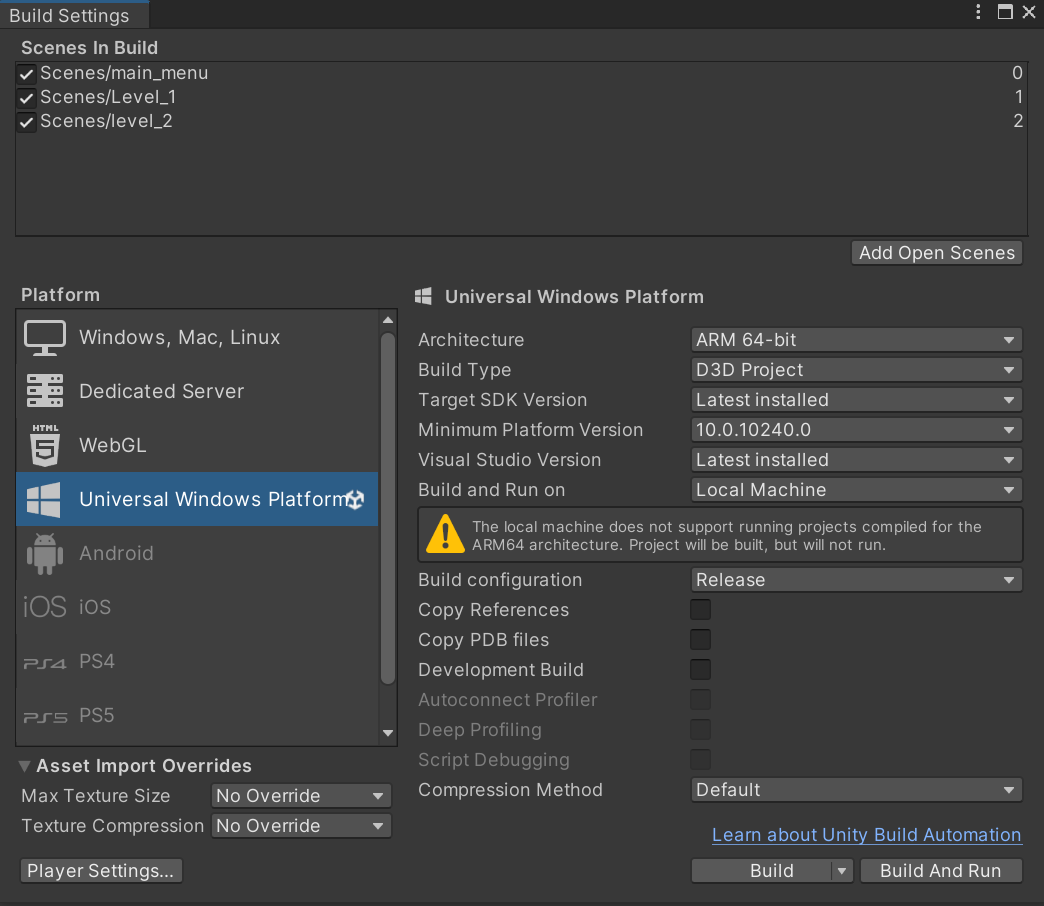
\includegraphics[scale=0.8]{images/build}
    \caption{Build-Einstellungen in Unity}
    \label{fig:build-settings}
\end{figure}

Nach einem erfolgreichen Build erhalten Sie einen Ordner mit den benötigten Dateien für das Deployment. Der nächste
Schritt erfolgt in der Visual Studio Solution, in unserem Fall \textit{AARIE.sln}. Nach dem Öffnen der Datei müssen die
Konfiguration auf \textit{Release} und die Plattform auf \textit{ARM64} eingestellt werden. Nachdem die Konfigurationen
vorgenommen wurden, muss die \textit{Machine Name} auf die lokale IPv4-Adresse der HoloLens gesetzt werden. Dies erfolgt in
den \textit{Projekteigenschaften} unter Debugging. Die IP-Adresse der HoloLens kann auf der Brille in den \textit{Einstellungen}
unter \textit{Netzwerk} gefunden werden.

Außerdem muss der \textit{Authentication Mode} auf \textit{Universal (Unencrypted Protocol)} gesetzt werden, um
sicherzustellen, dass die Kommunikation zwischen dem Computer und der HoloLens reibungslos erfolgt.

Nachdem alle Einstellungen vorgenommen wurden, kann die Anwendung auf die HoloLens deployt werden. Dazu muss die
Solution mit \textit{Start without Debugging} gestartet werden. Nach einem längeren Ladevorgang wird die Anwendung auf der
HoloLens geladen und gestartet.

Falls die Anwendung beendet wird, kann sie auf der HoloLens unter
\textit{Start} $\rightarrow$ \textit{Alle Apps} $\rightarrow$ \textit{AARIE} erneut gestartet werden.
Falls Änderungen an der Anwendung auf den Computern vorgenommen wurden, muss der gesamte Prozess erneut durchgeführt werden.
Die Anwendung wird nicht automatisch aktualisiert!

\subsubsection{Erstmaliges Deployment}
Beim erstmaligen Deployment auf die HoloLens kann es zu Problemen kommen, die durch die Authentifizierung der HoloLens
verursacht werden. In diesem Fall muss der neue Computer sich auf der HoloLens erneut authentifizieren. Dazu werden Sie nach
dem Starten des Deployments aufgefordert. Auf dem Computer wird ein Authentifizierungscode angezeigt, der auf der HoloLens unter
\textit{Einstellungen} $\rightarrow$ \textit{Update & Sicherheit} $\rightarrow$ \textit{Für Entwickler} $\rightarrow$ \textit{Koppeln}
eingegeben wird. Nachdem die Authentifizierung erfolgreich abgeschlossen wurde, kann das Deployment erneut gestartet werden.


\section{Objektdesign mit Blender}
Das Entwerfen von 3D-Objekten mit Blender erfordert ein Verständnis der Struktur und Funktionalität dieser leistungsstarken
Software. Im Folgenden wird erläutert, wie Blender aufgebaut ist, auf welche Aspekte bei der Gestaltung der Objekte geachtet
wurde und welche Add-ons und Plug-ins verwendet wurden, um den Designprozess zu optimieren.

\subsection{Optimierung für Augmented Reality}
Der Entwurf von 3D-Objekten mit Blender erfordert ein systematisches Vorgehen, insbesondere im Zusammenhang mit der
Optimierung für Augmented Reality (AR). Im Folgenden werden spezifische Aspekte dieses Prozesses beleuchtet, darunter
die Polygonreduktion und die Texturoptimierung.

\subsubsection{Polygonreduktion}
Die Polygonreduktion ist eine Technik, die darauf abzielt, die Anzahl der Polygone in einem 3D-Modell zu reduzieren, um
die Belastung der Hardware zu verringern, insbesondere bei Echtzeitanwendungen wie Computerspielen oder Simulationen.
Eine effiziente Polygonreduktion ermöglicht eine bessere Leistung und eine schnellere Darstellung der Modelle auf
verschiedenen Plattformen.

In der Computergrafik steht die Anzahl der Polygone eines Modells in direktem Zusammenhang mit dem benötigten Speicherplatz
und der Rechenleistung. Je mehr Polygone ein Modell hat, desto mehr Daten müssen verarbeitet und gerendert werden, was
zu höheren Anforderungen an die Hardware führt. Durch eine Reduzierung der Polygone können diese Ressourcen effizienter
genutzt werden, ohne dass die visuelle Qualität des Modells wesentlich beeinträchtigt wird.

Werkzeuge wie der Decimate Modifier in Blender bieten Möglichkeiten, die Anzahl der Polygone automatisch zu reduzieren
und gleichzeitig visuelle Artefakte zu minimieren. Dennoch ist es ratsam, bereits während des Modellierungsprozesses
darauf zu achten, keine unnötigen zusätzlichen Unterteilungen zu erzeugen, um eine optimale Ausgangsbasis für die
Polygonreduktion zu schaffen.

Die Polygonreduktion ist ein wichtiger Bestandteil der 3D-Modellierung und -Optimierung, da sie dazu beiträgt, die Leistung
von Anwendungen zu verbessern und die Benutzererfahrung zu optimieren. Durch eine sorgfältige Anwendung dieser Technik
können qualitativ hochwertige 3D-Modelle erstellt werden, die sowohl ästhetisch ansprechend als auch effizient zu verarbeiten
sind.

\subsubsection{Texturenoptimierung}
Die Optimierung von Texturen ist ein wesentlicher Bestandteil der Gestaltung von 3D-Modellen für Augmented Reality
(AR)-Anwendungen, da sie einen direkten Einfluss auf die Benutzererfahrung haben. Bei der Auswahl geeigneter Texturen
muss der Auflösung besondere Aufmerksamkeit geschenkt werden, insbesondere im Hinblick auf die begrenzte Leistungsfähigkeit
von AR-Geräten wie der Hololens 2.

Während des Texturierungsprozesses wurde die Hololens 2 mehrfach in die Texturen integriert, um mögliche Leistungseinbußen
zu identifizieren. Wurden Beeinträchtigungen festgestellt, wurden entsprechende Anpassungen an den Texturen vorgenommen.
Dies beinhaltete entweder die Suche nach alternativen Texturen oder die Komprimierung der vorhandenen Texturen, um eine
geringere Auflösung zu erreichen. In einigen Fällen wurde auch der Reflexionsgrad angepasst, insbesondere wenn das Modell
poliertes Metall oder ähnliches enthielt, um die Leistung der AR-Anwendung zu optimieren.

Die Texturoptimierung ist ein iterativer Prozess, der eine ausgewogene Berücksichtigung der visuellen Qualität und der
Leistungsfähigkeit der AR-Plattform erfordert. Durch die gezielte Optimierung von Texturen können AR-Anwendungen erstellt
werden, die eine ansprechende visuelle Darstellung bieten und gleichzeitig ein flüssiges und immersives Benutzererlebnis
gewährleisten.

\subsection{Export- und Integrationsprozess}
In diesem Abschnitt wird der Export- und Integrationsprozess für 3D-Modelle beschrieben, beginnend mit der Auswahl des
geeigneten Dateiformats und der Berücksichtigung verschiedener Koordinatensysteme.

Der Export- und Integrationsprozess ist ein entscheidender Schritt bei der Übertragung von 3D-Modellen aus der Konstruktions-
oder Modellierungssoftware in eine Zielumgebung, sei es eine Spiele-Engine, eine Virtual-Reality-Plattform oder eine AR-Anwendung.
Dieser Prozess umfasst mehrere Schritte, um sicherzustellen, dass das Modell korrekt dargestellt und funktional in die
Zielumgebung integriert wird.

\subsubsection{Dateiformat}
Als Dateiformat für den Export von 3D-Modellen in diesem Projekt wurde das von Autodesk entwickelte Filmbox-Format (FBX)
gewählt. FBX wurde aufgrund seiner weit verbreiteten Unterstützung und seiner Fähigkeit, umfassende Informationen über
geometrische Formen, Materialien, Animationen und andere Szenendaten zu speichern, ausgewählt.

FBX ist ein proprietäres Format, das speziell für den Austausch von 3D-Inhalten zwischen verschiedenen Anwendungen
entwickelt wurde. Es bietet eine hierarchische Struktur, die es ermöglicht, komplexe Szenen zu organisieren und zu
übertragen. Diese Struktur umfasst Knoten, die verschiedene Elemente der 3D-Szene repräsentieren, wie Geometrie,
Materialien, Animationen, Kameras und Lichtquellen.

Durch die Verwendung von FBX können 3D-Modelle nahtlos zwischen verschiedenen Softwareanwendungen und Plattformen
ausgetauscht werden, was die Zusammenarbeit und Integration in Projekten wie diesem, das Unity als Engine verwendet,
erleichtert. Die Wahl des FBX-Formats bietet somit eine solide Grundlage für einen effizienten Workflow und eine
erfolgreiche Umsetzung des Projekts.

\subsubsection{Koordinatensysteme}
Die Berücksichtigung und korrekte Handhabung von Koordinatensystemen während des Modellierungsprozesses ist ein
entscheidender Aspekt für die nahtlose Integration von 3D-Modellen in verschiedene Anwendungen. In diesem Projekt
wurden spezifische Maßnahmen ergriffen, um potenzielle Probleme im Zusammenhang mit Koordinatensystemen zu minimieren.

Während der Modellierung wurden alle Objekte im Koordinatenursprung platziert, um sicherzustellen, dass beim Export
der Modelle nach Unity keine Komplikationen hinsichtlich Platzierung und Ausrichtung auftreten. Diese Vorgehensweise
trägt dazu bei, mögliche Diskrepanzen zwischen den Koordinatensystemen der Modellierungssoftware und der Zielplattform
zu vermeiden, was den Integrationsprozess vereinfacht und beschleunigt.

Darüber hinaus wurden alle Modelle in der gleichen Ausrichtung modelliert, um zusätzliche Anpassungen in Unity zu
vermeiden. Diese konsistente Orientierung stellt sicher, dass alle Modelle bereits in einer standardisierten
Orientierung vorliegen, was die Notwendigkeit weiterer manueller Eingriffe minimiert und einen reibungsloseren
Arbeitsablauf gewährleistet.

Für den Fall, dass Modelle dennoch mit einer falschen Rotation exportiert wurden, wurden entsprechende Korrekturen
direkt im Unity Inspector vorgenommen. Diese Nachjustierung ermöglicht es, eventuelle Fehler in der Ausrichtung der
Modelle schnell und effizient zu beheben, ohne den Modellierungsprozess zu unterbrechen oder zusätzlichen Aufwand zu
verursachen.

Insgesamt zeigt die Berücksichtigung von Koordinatensystemen während des gesamten Workflows einen proaktiven Ansatz
bei der Modellierung und Integration von 3D-Objekten. Die Umsetzung dieser Maßnahmen wird die Konsistenz und Effizienz
des Projekts verbessern und gleichzeitig mögliche Komplikationen im Zusammenhang mit Koordinatensystemen effektiv
vermeiden.

\subsection{Add-Ons und Plugins}
Während der Modellierungsphase wurden einige Add-ons und Plug-ins verwendet, um die Erfahrung zu verbessern und die
Modellierung effizienter zu gestalten. Im folgenden Abschnitt werden die wichtigsten Add-ons und Plug-ins erläutert.

\subsubsection{Looptools: Optimierung von Topologie und Oberflächen}
Das Add-on Looptools \footnote{Blender \cite{LoopTools}} für Blender stellt eine wichtige Ergänzung für die
Flächenmodellierung und Topologieoptimierung dar. Insbesondere bei der Umwandlung von rechteckigen oder quadratischen
Flächen in kreisförmige Flächen erweist sich dieses Werkzeug als äußerst nützlich.

Als Hauptwerkzeug wurde das so genannte "Circle"-Werkzeug verwendet, das speziell zur Lösung des oben genannten Problems
entwickelt wurde. Mit dem "Circle"-Werkzeug können rechteckige Flächen unter Berücksichtigung der Topologie und der
Anzahl der Polygone nahtlos in kreisförmige Flächen umgewandelt werden.

Das Circle-Werkzeug bietet verschiedene Einstellungsmöglichkeiten, um die extrahierte Figur optimal für den jeweiligen
Zweck zu konfigurieren. Die wichtigsten Konfigurationspunkte sind

\begin{itemize}
    \item \textbf{Best Fit:} Dieses Werkzeug berechnet einen Kreis mit Hilfe einer nichtlinearen Methode der kleinsten
    \item Quadrate. Dadurch wird sichergestellt, dass der berechnete Kreis optimal zu den ausgewählten Eckpunkten passt.
    \item \textbf{Fit Inside:} Mit dieser Option wird der Kreis so berechnet, dass kein Eckpunkt vom Kreismittelpunkt
    \item entfernt wird. Dies ist besonders nützlich, wenn die Topologie des umgebenden Mesh erhalten bleiben soll.
\end{itemize}

Zusätzlich ermöglicht das Circle-Werkzeug die Anpassung weiterer Konfigurationsparameter wie Radius und Regularität, um
die extrahierte Figur feiner abzustimmen und besser an individuelle Anforderungen anzupassen.

Insgesamt trägt das Looptools Add-On dazu bei, den Modellierungsprozess effizienter zu gestalten und die Qualität der
resultierenden Modelle zu verbessern, indem es eine Reihe präziser und flexibler Werkzeuge für die Topologie- und
Flächenoptimierung bereitstellt.

\subsubsection{Images as Planes: Effiziente Integration von Texturen}
Das Addon Images as Planes \footnote{Blender \cite{Images as Planes}} spielt eine entscheidende Rolle in der
Modellierungspraxis, insbesondere im Bereich der realistischen Modellierung.

Das Hauptanwendungsgebiet dieses Add-ons liegt in der Möglichkeit, Vorschaubilder für die Modellierung hinter Objekten
zu platzieren, um eine realistischere und präzisere Modellierung zu ermöglichen. Diese Funktion bietet die Möglichkeit,
reale Bilder als Referenz in Blender-Szenen zu integrieren und als Hintergrund für die Modellierung zu verwenden. Durch
die direkte Integration von Bildern in die Arbeitsumgebung können feine Details und Proportionen besser beurteilt und
reproduziert werden, was zu einer verbesserten Qualität der Modelle führt.

Die Verwendung von "Images as Planes" trägt somit wesentlich zur Erhöhung der Genauigkeit und Realitätsnähe der
Modellierung bei, indem sie eine effiziente Möglichkeit bietet, reale Referenzen in den Modellierungsprozess zu integrieren.
Diese Funktion ist besonders nützlich bei der Modellierung von Objekten, die auf realen Vorbildern basieren, da sie es
dem Modellierer ermöglicht, direkt aus Bildern heraus zu arbeiten und so einen höheren Detaillierungsgrad zu erreichen.

Insgesamt ist das Addon "Images as Planes" ein unverzichtbares Werkzeug für die realistische Modellierung in Blender,
das die Effizienz und Qualität des Modellierungsprozesses erheblich verbessert. Durch die nahtlose Integration von Bildern
als Hintergrundreferenzen können Designer ihrer Kreativität freien Lauf lassen und präzise Modelle mit realistischen
Details erstellen.

\subsection{Modi}
In Blender stehen verschiedene Modi \footnote{Blender \cite{Modi}} zur Verfügung, mit denen unterschiedliche Aspekte
eines Objekts bearbeitet und manipuliert werden können. Diese verschiedenen Modi in Blender bieten eine umfassende Palette
an Werkzeugen und Funktionen, mit denen die Benutzer ihre 3D-Modelle auf vielfältige Weise bearbeiten und verfeinern können.

\subsubsection{Object-Modus}
Der Object-Modus ist der Standardmodus in Blender und steht für alle Arten von Objekten zur Verfügung. In diesem Modus
können grundlegende Transformationen wie Positionierung, Rotation und Skalierung sowie Duplizierung und andere
Objekteigenschaften bearbeitet werden.

\subsubsection{Edit-Modus}
Der Edit-Modus ist ein spezialisierter Modus zum Bearbeiten der Form eines Objekts. Hier können mithilfe verschiedener
Werkzeuge und Kontrollpunkte einzelne Vertices \footnote{Blender \cite{Vertices}}, Kanten und Flächen des Objekts
bearbeitet werden. Dies ermöglicht detaillierte Manipulationen und Anpassungen an der Geometrie des Objekts, was
insbesondere für die Modellierung von entscheidender Bedeutung ist.

\subsubsection{Texture-Paint-Modus}
Der Texture-Paint-Modus ist ein spezieller Modus, der es ermöglicht, Texturen direkt auf das Mesh
\footnote{Blender \cite{Mesh}} eines Objekts zu malen. Dieser Modus ist ausschließlich auf das Bearbeiten von Meshes
beschränkt und bietet eine intuitive Möglichkeit, Texturen im 3D-Viewport zu zeichnen und zu bearbeiten. Durch die
direkte Malerei auf dem Objekt können komplexe Texturen und Oberflächeneffekte einfach erstellt und angepasst werden.

\subsection{Hierarchie}
In der 3D-Modellierung bezieht sich Hierarchie auf die strukturierte Organisation von Objekten innerhalb einer Szene
oder eines Modells. Diese Hierarchie wird oft durch eine Baumstruktur dargestellt, in der übergeordnete Objekte
untergeordnete Objekte enthalten können. Die Hierarchie spielt eine entscheidende Rolle bei der Verwaltung und
Manipulation von Objekten sowie bei der Definition von Beziehungen zwischen ihnen.

\begin{itemize}
    \item \textbf{Eltern-Kind-Beziehungen:} Übergeordnete Objekte werden oft als Eltern bezeichnet und enthalten
    untergeordnete Objekte, die als Kinder bezeichnet werden. Diese Beziehung ermöglicht es, Transformationen wie
    Verschieben, Drehen und Skalieren auf das übergeordnete Objekt anzuwenden, welche dann auf seine untergeordneten
    Objekte übertragen werden. Diese Technik ist besonders nützlich für komplexe Strukturen wie Roboterglieder oder
    hierarchische Modelle.
    \item \textbf{Gruppierung:} Objekte können hierarchisch gruppiert werden, um sie logisch zu organisieren und ihre
    Handhabung zu erleichtern. Durch die Gruppierung ist es möglich, mehrere Objekte gleichzeitig auszuwählen, zu
    verschieben oder zu bearbeiten, ohne jedes einzelne Objekt separat manipulieren zu müssen.
\end{itemize}
Die Hierarchie ist ein grundlegendes Konzept in der 3D-Modellierung. Sie ermöglicht eine effiziente Organisation und
Manipulation von Objekten. Durch die kluge Nutzung von Hierarchien können komplexe Modelle erstellt und verwaltet werden.
Dies führt zu einer effizienteren Arbeitsweise und einer verbesserten Qualität der Ergebnisse.

\subsection{Modifier}
Modifier sind Werkzeuge oder Operationen, die auf Objekte in der 3D-Modellierung angewendet werden, um ihr Aussehen oder
Verhalten zu verändern, ohne die zugrunde liegende Geometrie dauerhaft zu ändern. Sie ermöglichen es den Modellierenden,
komplexe Effekte zu erzielen, ohne manuell jeden einzelnen Aspekt des Modells zu bearbeiten. Modifier sind ein wichtiger
Bestandteil vieler 3D-Modellierungssoftware und bieten eine Vielzahl von Funktionen zur Verbesserung des Modellierungsprozesses.
Die Verwendung von Modifiern bringt mehrere Vorteile mit sich:

\begin{itemize}
    \item \textbf{Non-destructive Bearbeitung:} Modifier werden auf das Modell angewendet, ohne die ursprüngliche
    Geometrie zu verändern. Dies ermöglicht es, Änderungen vorzunehmen und bei Bedarf zum ursprünglichen Zustand
    zurückzukehren.

    \item \textbf{Effizienzsteigerung:} Durch die Verwendung von Modifiern können komplexe Effekte und Veränderungen mit
    weniger manuellem Aufwand erreicht werden. Dies führt zu einem effizienteren Modellierungsprozess und spart
    Zeit und Ressourcen.

    \item \textbf{Experimentierfreude:} Da Modifier nicht-destruktiv sind, können sie leicht hinzugefügt, angepasst oder
    entfernt werden. Dies ermutigt dazu, verschiedene Optionen auszuprobieren und kreativ zu experimentieren, ohne
    Angst vor irreversiblen Änderungen haben zu müssen.
\end{itemize}

Beispiele für Modifier sind Subdivision Surface, Mirror, Bevel, Array und Boolean. Jeder Modifier hat spezifische
Anwendungsfälle und ermöglicht es den Modellierenden, eine Vielzahl von Effekten zu erzielen, von der Glättung von
Kanten bis zur Erstellung von komplexen Wiederholungsmustern.

Modifier sind ein wichtiger Bestandteil der 3D-Modellierung. Sie bieten eine flexible und leistungsstarke Möglichkeit,
Objekte zu bearbeiten und zu verbessern, ohne die Integrität des Modells zu beeinträchtigen. Die Verwendung von Modifiern
kann den Modellierungsprozess rationalisieren und die Kreativität der Modellierenden fördern.

% vielleicht sachen dazu wie polygonanzahl oder arbeitsstunden oder sowas idk
\subsection{Modellierung von Gegenständen für das Projekt}
Dieser Abschnitt beschreibt die für das Projekt in Blender modellierten Gegenstände sowie die dabei aufgetretenen Herausforderungen.

Zu Beginn des Projekts musste eine wichtige Entscheidung getroffen werden, nämlich wie viele Objekte modelliert werden
sollten. Es war wichtig, eine ausgewogene Anzahl zu wählen, die das Spiel nicht überladen, aber dennoch eine
Herausforderung für die Spieler darstellt. Nach eingehenden Recherchen und internen Abstimmungen wurde sich auf 11
Gegenstände geeinigt. Diese sollten alltägliche Gegenstände eines Schülers der HTBLuVA darstellen und den Spielern
einen Einblick in den Schulalltag bieten.

\subsubsection{Taschenrechner}
Um den Modellierungsprozess am Beispiel des Taschenrechners zu veranschaulichen, werden spezifische Schritte und
Überlegungen während des Prozesses erläutert. Der Prozess begann mit der Idee, den Taschenrechner als Teil des Projekts
zu integrieren. Anschließend wurde der Modellierungsumfang und die Art des Taschenrechners festgelegt. Dabei diente das
Casio FX-991 ESPLUS Modell als Referenz für das zu erstellende Modell.

\subsubsection*{Ausgangslage}
Im Modellierungsprogramm Blender war das Standardprojekt als Ausgangslage zu sehen. Es wurde bereits geringfügig
angepasst. Die Standardkamera und Lichtquelle, die für das Rendering innerhalb von Blender verwendet werden, wurden
entfernt, da sie für das finale Projekt in Unity nicht benötigt werden und unnötige Komplikationen verursachen könnten.
Je nach Anforderung des Modells wird eine geeignete Grundform wie beispielsweise ein Würfel, eine Fläche oder ein Zylinder
erstellt, um darauf aufbauend mit der eigentlichen Modellierung zu beginnen.

\begin{figure}[H]
    \centering
    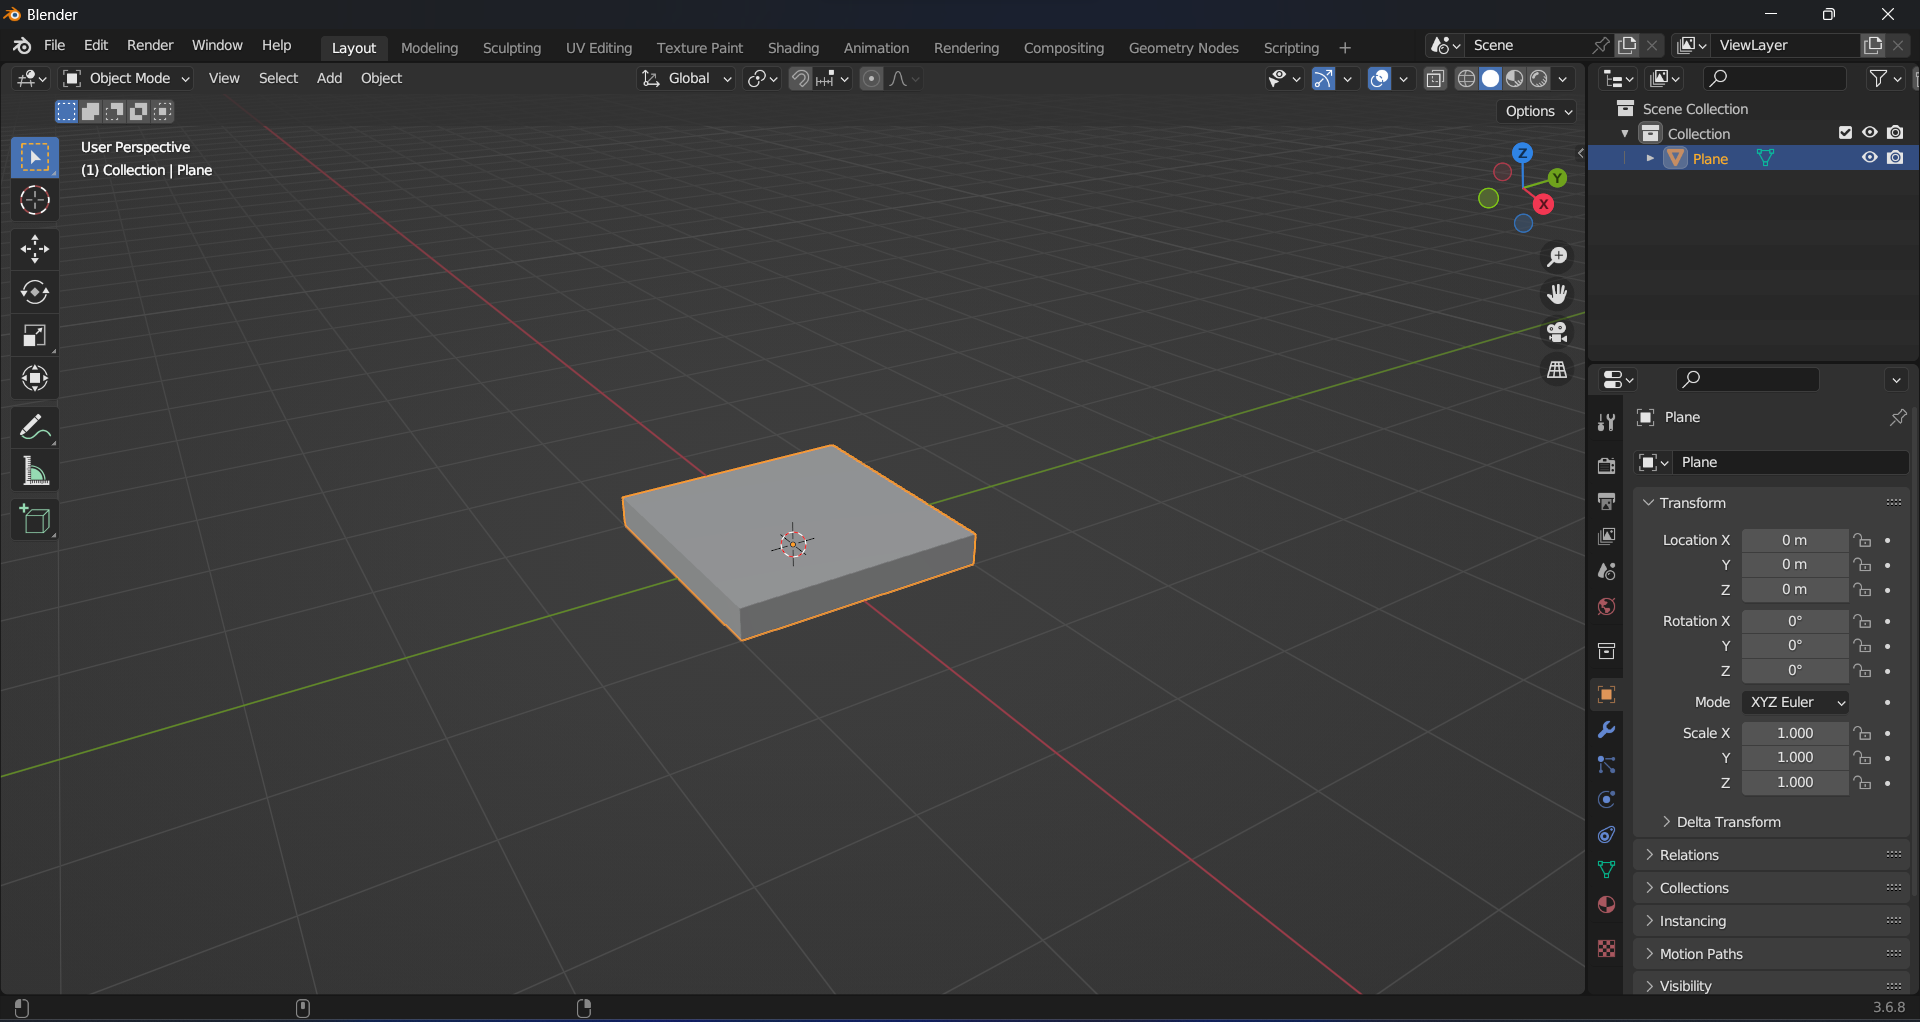
\includegraphics[width=1\textwidth]{images/AusgangslageTaschenrechner.png}
    \caption{Ausgangslage innerhalb von Blender}
    \label{fig:Ausgangslage}
\end{figure}

Durch diesen Prozess der Initiierung wurde die Grundlage für die folgenden Schritte der Modellierung gelegt, die in
weiteren Abschnitten detaillierter beschrieben werden.

\subsubsection*{Erste Schritte nach der Erstellung}
Nach Auswahl eines geeigneten Referenzbildes für das Taschenrechnermodell wurde dieses mithilfe des
Add-Ons \textit{Images as Planes} in Blender eingefügt. Das Bild dient als Leitfaden für die Modellierung und wurde
unterhalb des bereits vorhandenen Objekts platziert. Um eventuelle Unregelmäßigkeiten im Design zu vermeiden, wurde der
Mirror Modifier aufgrund der symmetrischen Form des Taschenrechners angewendet. Durch diese Maßnahme werden alle
Modellierungsaktionen, die auf einer Seite durchgeführt werden, automatisch auf die andere Seite gespiegelt. Dadurch
wird die Effizienz des Modellierungsprozesses erhöht.

Im Anschluss begann die Modellierung durch Extrudieren eines Eckpunkts der Fläche, um grob der Form des Referenzbildes zu folgen.

\begin{figure}[H]
    \centering
    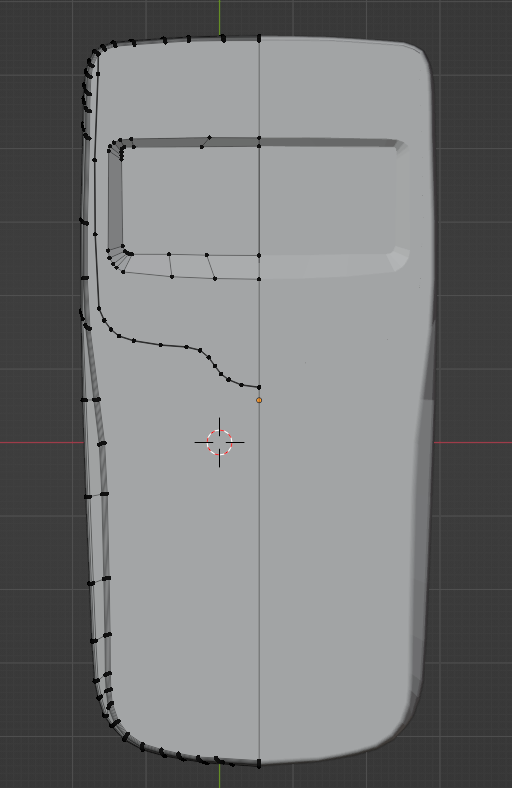
\includegraphics[width=0.4\textwidth]{images/basis.png}
    \caption{Taschenrechner mit Buttons in Blender}
    \label{fig:Basis}
\end{figure}


Nach Abschluss dieser groben Modellierungsschritte entstand das Grundgerüst des Taschenrechnermodells, wie in
Abbildung \ref{fig:Basis} dargestellt. Die verschiedenen Eckpunkte (Vertices) werden im Edit-Modus von Blender als
schwarze Punkte dargestellt. Durch den Mirror Modifier wird die Bearbeitung auf der linken Seite des Modells
automatisch auf die rechte Seite gespiegelt, was eine symmetrische Form gewährleistet. Um dem Modell mehr Tiefe zu
verleihen, wurde Extrudieren verwendet, um aus der ebenen Fläche eine dreidimensionale Struktur zu formen.

\subsubsection*{Extrahieren als Modellierungswerkzeug}
Extrahieren \footnote{Blender \cite{Extrahieren}} ist ein Werkzeug im Edit-Modus von Blender. Es dient dazu,
ausgewählte Punkte zu duplizieren und zu verschieben, während die ursprünglichen Punkte der Bearbeitungslinie erhalten bleiben.
Für die Verwendung des Extrahieren-Werkzeugs ist ein Verständnis der grundlegenden Konzepte des Edit-Modus in Blender
sowie eine präzise Auswahl der zu extrahierenden Punkte erforderlich, um die gewünschten Modifikationen am Modell
vorzunehmen. Während des Modellierungsprozesses ist es von entscheidender Bedeutung, unbeabsichtigte Extraktionen zu
vermeiden, da diese dazu führen können, dass duplizierte Vertices über bereits vorhandenen liegen. Dies kann nicht
nur die weitere Bearbeitung des Modells beeinträchtigen, sondern auch zu einer unnötigen Zunahme der Anzahl der
Vertices führen.

\subsubsection*{Weiterführung beim Taschenrechnermodell}
Als nächster Schritt steht die Modellierung der Knöpfe und anderer Funktionen des Taschenrechners an, um das Modell
weiter zu verfeinern und seinem realen Gegenstück näherzukommen. Dazu wird der \textit{Array}-Modifier verwendet, da
dieser es ermöglicht, ein Button-Modell zu entwerfen und dieses dann zu vervielfältigen. Dadurch wird die
Modellierungszeit enorm reduziert und die gleichmäßige Platzierung der Buttons verbessert.

\subsubsection*{Einschub Array-Modifier}
Der Array-Modifier in Blender ermöglicht die Erstellung einer Reihe von Kopien eines Basisobjekts. Jede Kopie wird dabei
auf eine vordefinierte Weise von der vorherigen Kopie versetzt. Der Modifier bietet eine Vielzahl von Optionen zur
Anpassung der Positionierung und Ausrichtung der Kopien.
Die grundlegenden Funktionen des Array-Modifiers umfassen die Möglichkeit, Vertices in benachbarten Kopien zusammenzuführen,
insbesondere wenn sie nahe beieinander liegen. Dadurch können nahtlose und konsistente Verbindungen zwischen den
einzelnen Kopien hergestellt werden.
Eine wichtige Option des Array-Modifiers ist der sogenannte \textit{Fit Type}, der angibt, wie das Objekt dupliziert
werden soll. Dies kann entlang einer Kurve, mit einer passenden Länge oder einer festgelegten Anzahl von Kopien erfolgen.
Darüber hinaus kann eine relative oder feste Verschiebung entlang der x-, y- oder z-Achse definiert werden, um die
Positionierung der Kopien weiter anzupassen.

\subsubsection*{Weiterführung beim Taschenrechnermodell}
\begin{figure}[H]
    \centering
    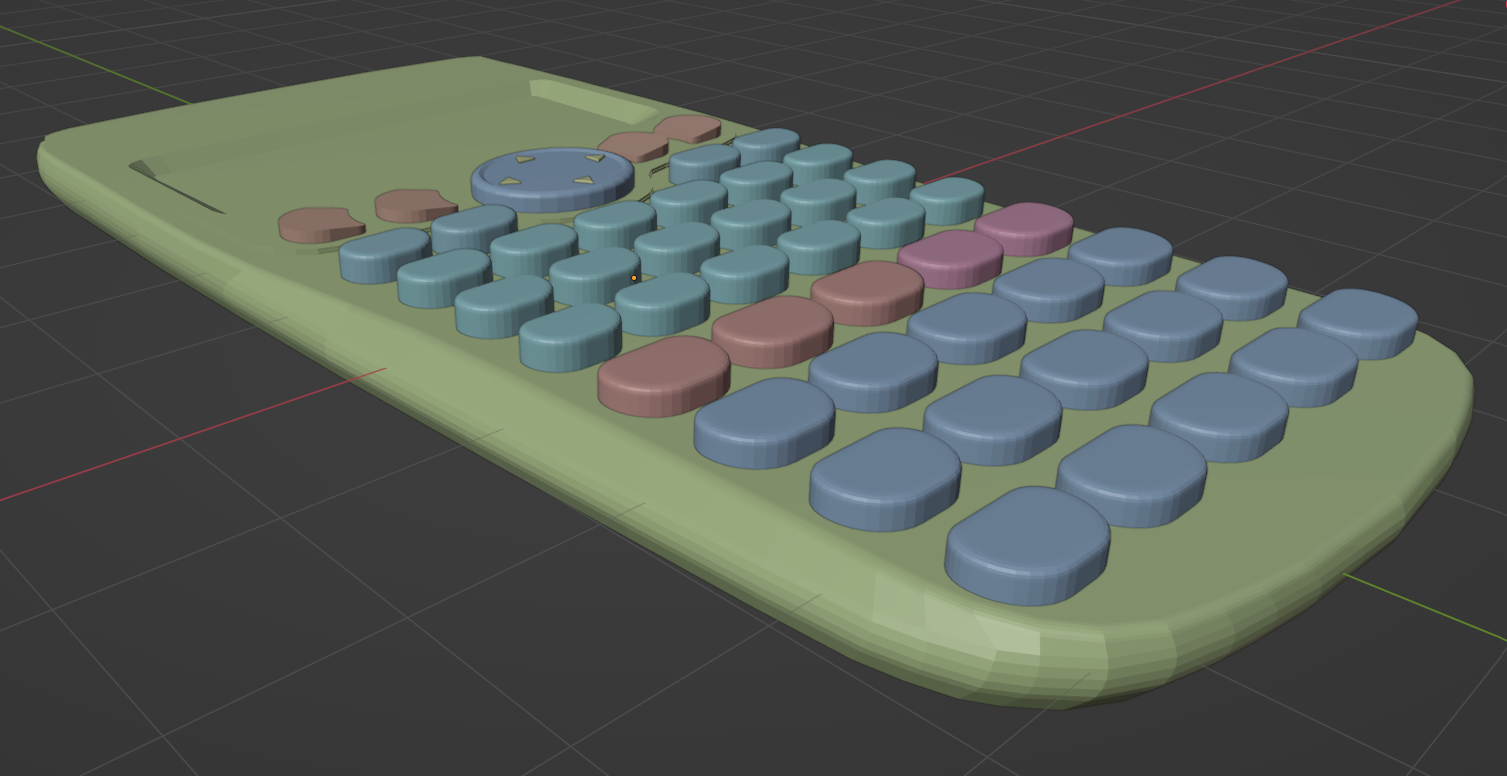
\includegraphics[width=0.8\textwidth]{images/taschenrechnermitbuttons.png}
    \caption{Taschenrechner mit Buttons in Blender}
    \label{fig:tcbuttons}
\end{figure}

Abbildung \ref{fig:tcbuttons} zeigt das Taschenrechnermodell in Blender mit den neu modellierten Buttons. Die
dargestellten Farben dienen lediglich als visuelle Hilfestellung im Blender-Editor und stellen keine inhärenten
Eigenschaften des Modells dar. Jedes neu erstellte Objekt wird automatisch mit einer zufälligen Farbe versehen, um eine
einfachere Unterscheidung innerhalb der Szene zu ermöglichen.

Einige der Buttons im Modell wurden mithilfe des Array-Modifiers vervielfältigt. Dies gilt insbesondere für Buttons, die
im Referenzbild die gleiche Größe, Funktion und Farbe aufweisen. Durch diese Technik ist es möglich, wiederkehrende
Elemente effizient zu modellieren, indem eine einzelne Vorlage kopiert und entsprechend der gewünschten Anordnung angepasst wird.

Der aktuelle Stand des Modells lässt darauf schließen, dass die Modellierung größtenteils abgeschlossen ist. Der nächste
Schritt besteht darin, dem Modell Farben oder Texturen hinzuzufügen, um ein realistischeres Aussehen zu erzielen. Dies
kann durch Anwendung von Materialien und Texturen im Renderprozess erreicht werden, um dem Modell visuelle Tiefe und
Detailtreue zu verleihen.

Die Fortführung des Modellierungsprozesses umfasst somit die Umsetzung der texturierten Oberfläche sowie mögliche
Feinanpassungen, um das Modell weiter zu verbessern und an die Referenzvorlage anzupassen.

\subsubsection*{Hierarchie des fertiggestellten Modells}
In Blender wird die Hierarchie eines Modells als Baumstruktur dargestellt. Dabei ermöglichen verschiedene Unterteilungen
und Kategorien eine übersichtliche Organisation. Die Struktur wird in Abbildung
\ref{fig:hierarchie} veranschaulicht. Das weiße Box-Symbol steht für eine Collection (Ordner).

\begin{figure}[H]
    \centering
    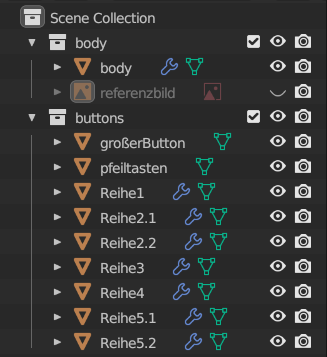
\includegraphics[width=0.5\textwidth]{images/hierarchietaschenrechner.png}
    \caption{Hierarchie des fertigen Taschenrechnermodells}
    \label{fig:hierarchie}
\end{figure}

\begin{itemize}
    \item Die \textbf{Scene Collection} ist die oberste Ebene, die das gesamte Modell enthält.
    \item Die \textbf{Body Collection} enthält das Hauptmodell des Taschenrechners, also die grundlegende Form.
    \item Die \textbf{Buttons Collection} umfasst alle Buttons, die auf dem Taschenrechner abgebildet sind.
    \item Die untergeordnete Struktur mit den orangefarbenen Dreiecken repräsentiert die eigentlichen Objekte innerhalb der jeweiligen Collections.
    \item Das \textbf{Referenzbild} ist ein importiertes Bild, an dem sich während des Modellierens orientiert wurde.
\end{itemize}

In Abbildung \ref{fig:hierarchie} ist zu erkennen, dass ein Objekt ausgegraut ist. Dies bedeutet in dem Fall, dass das
Objekt ausgeblendet wurde, da das Hauptmodell bereits fertiggestellt wurde und das Referenzbild nicht mehr benötigt wird.
Das Referenzbild kann jedoch bei Bedarf aktiviert werden, beispielsweise zu Hilfe- oder Veranschaulichungszwecken.

Die hierarchische Darstellung der Elemente erleichtert die Organisation und Bearbeitung des Modells. Eine klare
Strukturierung der verschiedenen Komponenten ermöglicht eine effiziente Arbeitsweise und hilft, den Überblick über die
einzelnen Teile zu behalten.

\subsubsection*{Textur und Farbe des Taschenrechnermodells}
Für die Texturierung und Farbgebung des Modells wurde sich eng an dem Referenzbild orientiert.
Das \textit{Eye-Dropper}-Werkzeug in Blender ermöglichte es, Farben gezielt aus dem Referenzbild auszuwählen und auf das
entsprechende Modell anzuwenden. Durch Klicken auf einen bestimmten Bereich des Referenzbildes wurde die Farbe erfasst
und dann auf den entsprechenden Bereich des Modells übertragen.

Dieser Prozess wurde für jedes Element des Modells durchgeführt, um eine genaue Anpassung an die Farben und Texturen
des Referenzbildes zu erreichen. Die Verwendung des Eye-Dropper-Werkzeugs ermöglichte eine präzise und konsistente
Umsetzung der Farbgebung und trug dazu bei, dass das Modell möglichst authentisch und realitätsnah aussieht.

%TODO: maybe UV-Mapping wegen Tasten und dann viel zum schreiben

\subsubsection{Restlichen Modelle}
\subsubsection*{Ping-Paket-Modell}
Das Ping-Paket-Modell wurde speziell für didaktische Zwecke auf Level 1 konzipiert, um Spielern das grundlegende Konzept
eines Daten-Pings zu veranschaulichen. Es dient dazu, die Übertragung von Daten zwischen zwei Endpunkten, beispielsweise
Laptops, zu visualisieren. Das Modell besteht im Wesentlichen aus einem simplen Quader, ergänzt durch Details wie
Paketklebeband, um eine realistische Darstellung zu erreichen. Bei der Texturierung wurde ein Amazon-Paket als Referenz verwendet.

\subsubsection*{Laptop-Modell}
Der Laptop stellt einen unverzichtbaren Gegenstand auf Level 2 dar und ist ein essenzielles Werkzeug für Schüler ab der
3. Klasse. Bei der Modellierung wurden zusätzliche Details wie USB-Ports und der Laptopständer berücksichtigt. Um den
Aufwand zu minimieren, wurde der Laptop im geschlossenen Zustand modelliert, wodurch die Komplexität von Tastatur und
Bildschirm vermieden wurde. Die Referenz für das Modell lieferte ein reales Laptop-Exemplar eines Projektmitglieds.

\subsubsection*{Router-Modell}
Die Modellierung des Routers war eine iterative Aufgabe, die mehrere Versionen erforderte, um ein realistisches und
ansprechendes Modell zu erzielen. Das finale Modell repräsentiert einen Gaming-Router mit vielen Anschlüssen und Bedienelementen.
Aufgrund der Vielzahl an Details war die Modellierung sehr anspruchsvoll und zeitaufwendig.

\subsubsection*{Maus-Modell}
Die Modellierung der Maus war eine Standardaufgabe, bei der der Mirror Modifier effektiv eingesetzt wurde, um die
symmetrische Natur des Objekts zu betonen. Eine einfache Büromaus diente als Referenz für das Modell.

\subsubsection*{Block-Modell}
Der Block ist ein wichtiger Gegenstand im schulischen Umfeld bis zur 3. Klasse, wenn noch keine Laptops verwendet werden.
Während der Designphase ermöglichte der Array Modifier eine einfache Gestaltung der spiralförmigen Halterung der Blätter.

\subsubsection*{Stift-Modell}
Der Stift wurde einfach modelliert und erhielt eine unkomplizierte Texturierung mit einfachen Farben. Ein Buntstift
diente als Referenz für das Modell.

\subsubsection*{Kopfhörer-Modell}
Die Modellierung der Kopfhörer erforderte aufgrund ihrer geschwungenen Form und der texturierten Oberfläche besondere
Aufmerksamkeit. Das Modell durchlief zwei Phasen: zunächst eine Annäherung an das Referenzbild eines Gaming-Kopfhörers
und dann eine Verfeinerung, einschließlich einer aufwendigen Lederstrukturtextur.

\subsubsection*{Dose-Modell}
Die Modellierung der Energydose begann mit einem einfachen Zylinder, der dann anhand eines Referenzbildes geformt wurde.
Besonderes Augenmerk wurde auf die Textur gelegt, wobei ein Redbull-Label als Referenz diente.

\subsubsection*{USB-Stick-Modell}
Der USB-Stick wurde mit einer integrierten Halterung für zusätzliche Komplexität modelliert. Die Texturierung betonte
einen metallischen Effekt, insbesondere für die Halterung und das vordere Teil des USB-Sticks.

\subsubsection*{Verteiler-Modell}
Der Stromverteiler wurde mit fünf Steckplätzen und einem Ein/Aus-Schalter modelliert, wobei der Fokus auf einfacher
Funktionalität lag. Die Texturierung orientierte sich an einfachen weißen Steckerleisten.

\subsubsection*{Handy-Modell}
Das Handymodell orientierte sich an modernen iPhones von Apple und erforderte aufgrund seiner zahlreichen Details wie
Kameras, Tasten und Mikrofoneinlässe eine sorgfältige Modellierung und Texturierung, um einen realistischen Eindruck zu erzeugen.


\section{Hauptmenü}
Im folgenden Abschnitt werden die Entwicklungsphasen beim Entwerfen des Menüs erläutert. So wie die dabei aufgetretenen
Probleme und abschließend auch auf was beim User interface UI under bei der Benutzererfahrung UX geachtet wurde.
Die iterative Entwicklung des Menüs durchlief mehrere Phasen, beginnend mit der Konzeption und Planung der
Benutzeroberfläche bis hin zur finalen Umsetzung. Dieser Prozess umfasste die Entscheidungen zum Design des Layouts, des
Farbschemas und der Interaktionselemente. Während der Entwicklung wurden regelmäßig Überprüfungen und Anpassungen
vorgenommen, um sicherzustellen, dass das Menü den gestellten Anforderungen entspricht und eine optimale Benutzererfahrung
bietet. Dabei wurden auch Rückmeldungen und Tests von Nutzern in die Iterationsschleife einbezogen, um mögliche
Verbesserungspotenziale zu identifizieren und zu berücksichtigen.
Schließlich wurde das Menü in seiner finalen Version implementiert. Dabei wurde besonderes Augenmerk auf Funktionalität,
Benutzerfreundlichkeit und Ästhetik gelegt. Durch diesen iterativen Entwicklungsprozess wurde sichergestellt, dass das
Menü den Anforderungen entspricht und einen positiven Beitrag zur Gesamterfahrung des Spiels leistet.

\subsection{Erstentwurf}
Ursprünglich war geplant, das UI/UX-System mit einem sogenannten \textbf{Nahmenü} zu realisieren. Dieses folgt dem
Nutzer in seiner Nähe und besteht in unserem Fall, aus drei primären Schaltflächen sowie einem Pin-Button. Das Nahmenü
ist etwa auf Hüfthöhe des Benutzers positioniert und zeichnet sich durch eine vereinfachte Struktur aus, die eine
intuitive Bedienung gewährleistet. Die Gestaltung des Menüs hat zum Ziel, Verwirrung zu vermeiden und dem Nutzer ohne
umfassende Vorabinformationen klar zu machen, wie er es verwenden kann.

\subsubsection*{Nahmenü}
Innerhalb von Unity bezeichnet der Begriff Nahmenü eine vordefinierte Konstruktion, die mit bestimmten Skripten
ausgestattet ist, um sicherzustellen, dass das Menü dem Benutzer in alle Richtungen folgt. Es werden von Unity
bereitgestellte Skripte verwendet, die es ermöglichen, das Menü dynamisch an die Position des Nutzers anzupassen.\\
\\
Im Erstentwurf wurde das gesamte Menü ausschließlich innerhalb der Unity-Umgebung konstruiert. Dabei wurden sämtliche
vorhandenen Schaltflächen und Funktionen aus den nativen Ressourcen von Unity zusammengesetzt. Dieser Ansatz führte zu
einer konsistenten visuellen Gestaltung des Menüs. Allerdings waren die Möglichkeiten zur kreativen Gestaltung und
Anpassung im Rahmen unseres individuellen Projekts stark begrenzt. Durch die ausschließliche Verwendung der internen
Ressourcen von Unity wurden gewisse Einschränkungen hinsichtlich der Flexibilität und Individualisierungsmöglichkeiten
des Menüs in Kauf genommen.

Obwohl diese Herangehensweise zu einem homogenen Erscheinungsbild des Menüs führte, war es wichtig, eine Balance
zwischen visueller Einheitlichkeit und der Notwendigkeit individueller Anpassungsmöglichkeiten zu finden. Diese
Herausforderung verdeutlicht die Bedeutung einer flexiblen und erweiterbaren Architektur für die Benutzeroberfläche,
um den Anforderungen und Zielen des Projekts gerecht zu werden.
\begin{figure}[H]
    \centering
    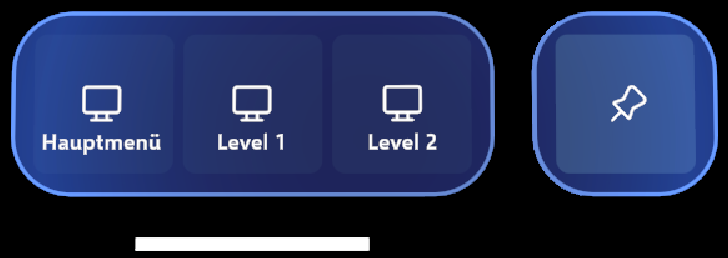
\includegraphics[width=0.8\textwidth]{images/menubarversion1.png}
    \caption{Darstellung des Erstentwurfes im Unity Editor}
    \label{fig:menübar}
\end{figure}

Die Abbildung \ref{fig:menübar} zeigt den ersten Entwurf des Menüs, das eine wichtige Schnittstelle für den Nutzer
darstellt, um zwischen verschiedenen Szenarien zu navigieren. Die Struktur des Menüs bleibt unabhängig vom jeweiligen
Spiellevel konstant, was zur Simplifizierung und Klarheit beiträgt. Die primären Schaltflächen auf der linken Seite
dienen der Initiation des Ladevorgangs für die verschiedenen Spielszenarien. Hervorzuheben ist der Pin-Button in
Kombination mit dem darunterliegenden weißen Balken. Diese beiden Funktionen gemeinsam ermöglichen es dem Benutzer,
das Menü an gewünschten Positionen zu verankern und bietet somit Flexibilität bei der Positionierung entsprechend
individueller Präferenzen. Ein solcher Einsatz ist von Vorteil, wenn externe Objekte die Nutzbarkeit des Menüs
beeinträchtigen könnten, wie zum Beispiel im Szenario des Platznehmens an einem Tisch, wo das Menü ungünstigerweise
mit dem Tisch kollidieren könnte und somit die Nutzererfahrung beeinträchtigt werden würde.

\subsubsection{Probleme beim Erstentwurf}
\subsubsection*{Problem 1 - Fehlende Dokumentation}
Das Hauptziel bei dem Konzept des Ersten Menüs, bestand darin, ein benutzerfreundliches Menü zu gestalten, das alle
erforderlichen Funktionen enthält und dennoch übersichtlich ist. Nach mehreren Iterationen und Tests mit Testpersonen,
die nicht mit dem Projekt vertraut waren, stellte sich heraus, dass der ursprüngliche Entwurf erhebliche Mängel bei der
Dokumentation und Erklärung der verschiedenen Anwendungsszenarien und ihrer jeweiligen Aufgaben aufweist. Es wurde
bemängelt, dass Benutzer lediglich zwischen den einzelnen Leveln wechseln können, ohne klare Informationen darüber zu
erhalten, worum es in den einzelnen Leveln geht und welche Aufgaben diese beinhalten.

Diese Feststellung verdeutlicht eine wesentliche Lücke in der Benutzerführung und -information innerhalb des Menüsystems.
Die unzureichende Dokumentation der Level und ihrer Ziele führt zu einer fehlenden Orientierung für die Benutzer und
kann sich negativ auf ihre Erfahrung auswirken. Das Menü sollte nicht nur als Navigationswerkzeug dienen, sondern auch
als Informationsquelle, die dem Benutzer eine klare Vorstellung über den Spielverlauf und die zu erreichenden Ziele vermittelt.

Die Identifizierung dieses Problems betont die Wichtigkeit einer umfassenden Benutzerforschung und -evaluation während
des Designprozesses. Dadurch wird sichergestellt, dass das entwickelte Benutzeroberflächensystem den Bedürfnissen und
Erwartungen der Zielgruppe entspricht. Eine zielgerichtete Überarbeitung des Menüs ist erforderlich, um die fehlende
Dokumentation der Anwendungsszenarien und ihrer Aufgaben zu adressieren und somit die Benutzererfahrung zu verbessern.

Bei Testdurchführungen ohne Entwickler aus dem Projektteam kam es wiederholt zu Unklarheiten bei den Benutzern,
insbesondere während des ersten Durchlaufs, bezüglich der zugewiesenen Aufgaben. Während der Nutzung der HoloLens-Anwendung
gab es vermehrt Anfragen seitens der Benutzer an das Projektteam aufgrund von Unklarheiten. Dies lässt vermuten, dass
die Anwesenheit von Entwicklern im Projektteam einen signifikanten Einfluss auf die Benutzererfahrung und Effektivität
der HoloLens-Anwendung hat.


\subsubsection*{Problem 2 - Falsche Wahl des Menütyps}
Während des Testprozesses stellte sich heraus, dass das Navigationsmenü oft eine Behinderung darstellte, insbesondere
für Entwickler, die Funktionen wiederholt testeten und Anwendungsszenarien neu luden. Das ständige Verschieben des Menüs
zur Seite erwies sich als zeitraubend und störte den Arbeitsfluss erheblich. Die ursprüngliche Intention, das
Navigationsmenü zur Erleichterung der Interaktion zwischen Benutzer und Spielumgebung einzuführen, erwies sich somit als kontraproduktiv.

Es ist wichtig, die Auswirkungen von Benutzeroberflächenelementen auf den Entwicklungsprozess zu berücksichtigen, um ein
reibungsloses Testen und Experimentieren zu gewährleisten. Eine effiziente und produktive Arbeitsweise des
Entwicklerteams hängt davon ab. Die Notwendigkeit einer kontinuierlichen Evaluation und Optimierung von
UI/UX-Komponenten während des gesamten Entwicklungszyklus wird durch dieses Problem verdeutlicht.

Dieses Problem verdeutlicht, dass der Erstentwurf und die ursprüngliche Konzeption hauptsächlich auf die Innovation und
Neuheit des Menüdesigns abzielten, anstatt den Fokus auf die funktionale Nützlichkeit zu legen. Der einfache und kompakte
Menütyp erwies sich als unzureichend, um eine umfassende und übersichtliche Dokumentation der Anwendungsszenarien zu
integrieren. Folglich war eine Migration zu einem alternativen Menüansatz erforderlich. Diese Beobachtung verdeutlicht
die Bedeutung einer ausgewogenen Gestaltung von Benutzeroberflächen in Mixed-Reality-Systemen. Es ist wichtig, dass
nicht nur ästhetische Innovationen verfolgt werden, sondern auch die tatsächliche Benutzererfahrung und -effizienz in
Betracht gezogen wird. Die Reflexion über diesen Prozess bietet Einsichten in die iterative Entwicklung von
Benutzerschnittstellen und die Anpassung an die Anforderungen und Rückmeldungen der Benutzer.

\subsection{Finalversion des Menüs}
Die endgültige Version des Menüs wurde entwickelt, um die Mängel des ursprünglichen Entwurfs anzugehen und idealerweise
vollständig zu beheben. Dieses neue Konzept wurde durch eine umfassende Analyse populärer AR/VR-Spiele geleitet, um die
Gründe für die verbesserte Benutzererfahrung in diesen Kontexten zu untersuchen. Dabei wurden spezifische Merkmale und
Designentscheidungen identifiziert, die einen signifikanten Einfluss auf die Zufriedenheit der Anwender haben.

Basierend auf vorangegangenen Recherchen wurde entschieden, das neue Menü in zwei klar definierte Bereiche zu unterteilen.
Dies gewährleistet eine deutliche Unterscheidung des Hauptmenüs sowie eine klare Orientierung bezüglich der Navigation.
Insbesondere innerhalb der Anwendungsszenarien wurde ein minimalistisches und unaufdringliches Menü implementiert, um
den Fokus der Benutzer uneingeschränkt auf die auszuführenden Tätigkeiten zu lenken. Diese Designstrategie hat zum Ziel,
die kognitive Belastung der Benutzer zu reduzieren und eine nahtlose Integration der Menüfunktionalitäten in den jeweiligen
Nutzungskontext zu ermöglichen.

Das Ergebnis ist ein ansprechendes und benutzerorientiertes Menükonzept, das die Gesamterfahrung des Spiels verbessert
und den Erwartungen der Zielgruppe gerecht wird.

\subsubsection{Finalversion Menü - Hauptmenü}
Auf dieser Grundlage wurde das Design des Menüsystems vollständig überarbeitet, wobei der erste Schritt schonmal die
vollständige Entfernung der Idee des Nahmenüs beinhaltet.

Anstelle des Nahmenüs wurden vorgefertigte Objekte in das Hauptmenü integriert, welche zuvor mit Blender modelliert wurden.
Die Entscheidung, vorgefertigte Objekte aus Blender zu importieren, bietet eine breite Palette an Gestaltungsmöglichkeiten
und ermöglicht es, das Menü visuell ansprechend und einladend zu gestalten. Außerdem trägt die Integration dieser Objekte
dazu bei, das Menü intuitiver und zugänglicher zu machen, indem sie dem Benutzer klare Anhaltspunkte und Handlungsmöglichkeiten bieten.

\begin{figure}[H]
    \centering
    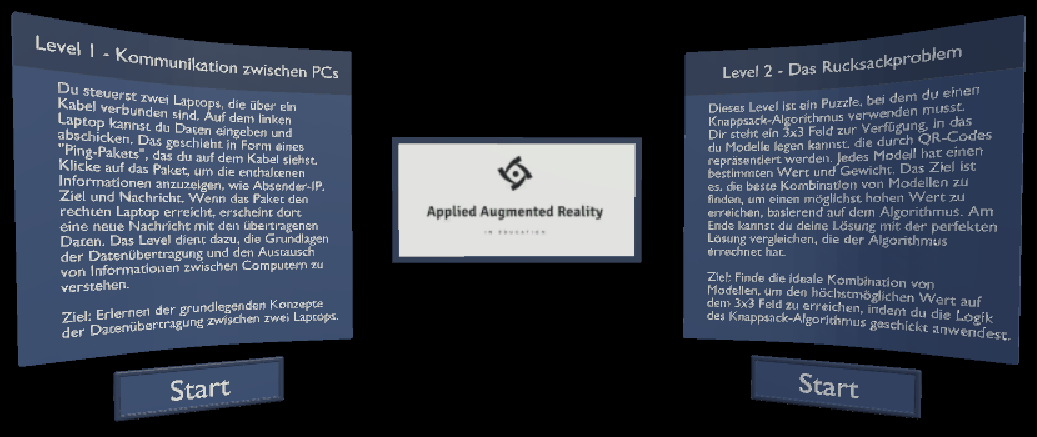
\includegraphics[width=1\textwidth]{images/menuversion2.png}
    \caption{Darstellung des Finalen Menüs im Unity Editor}
    \label{fig:menuversion2}
\end{figure}

Die in der Abbildung \ref{fig:menuversion2} dargestellten Objekte bestehen aus zwei separaten Tafeln, die durch unser
Diplomarbeitslogo voneinander getrennt sind. Jede Tafel enthält den Titel des Anwendungsszenarios sowie einen vorgefertigten
Startbutton.  In Unity wurde ein unsichtbarer, aber dennoch klickbarer Button mit exakt denselben Dimensionen wie das
Modell des Startbuttons an der entsprechenden Stelle platziert. Das Skript \textit{SceneChange.cs}, welches für die
Szenenwechsel-Funktionalität verantwortlich ist, ist diesem Button angehängt.

\begin{figure}[H]
    \centering
    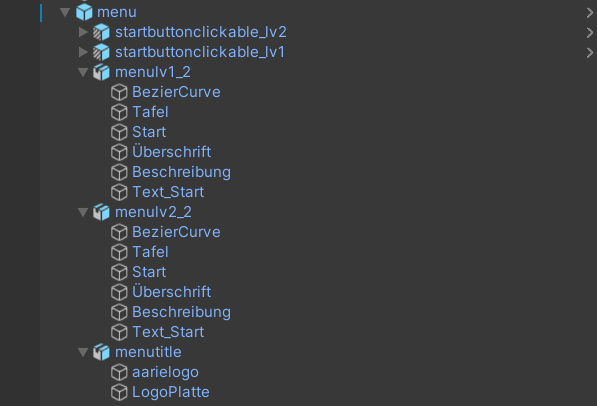
\includegraphics[width=0.8\textwidth]{images/hierarchiemenuunity.png}
    \caption{Darstellung der Hierarchie des finalen Menüs im Unity Editor}
    \label{fig:hierarchiemenuunity}
\end{figure}

In der Abbildung \ref{fig:hierarchiemenuunity} ist die Hierarchie des Hauptmenüs im Unity Editor zu sehen. Dem
Prefab \textbf{menu} sind dabei 5 einzelne Objekte zugewiesen. Die Prefabs \textbf{startbuttonclickable\_lv1/2} sind die
in Unity erstellen unsichtbaren Button die dafür zuständig sind den vormodellierten Buttons eine Funktion zu geben. Darunter
zu sehen sind die 3 verschiedenen Assets welche aus blender importiert wurden. Diese bestehen jeweils aus den verschiedenen
Einzelteilen, welche in Unity als Gameobjects dargestellt werden. Die \textbf{BezierCurve} ist eine spezielle Art von Kurve
welche in Blender für die leichte Wölbung der Tafeln genutzt wurde.

\subsubsection{Finalversion Menü - Anwendungsszenario}
Im Gegensatz zum Erstentwurf, der ein einheitliches Menü für alle Anwendungsszenarien vorsah, weist diese Version eine
Differenzierung auf. Die Entscheidung, das Menü innerhalb der einzelnen Szenarien anzupassen, wurde getroffen, um die volle
Aufmerksamkeit des Benutzers auf das jeweilige Level und die darin ausgeführten Aktivitäten zu lenken. Aus diesem Grund
wurde ebenfalls das Nahmenü aus den Szenarien entfernt und durch ein simples Handmenü ersetzt.

\begin{figure}[H]
    \centering
    
\includegraphics[width=0.8\textwidth]{images/backbutton.png}
    \caption{Darstellung des Finalen Menüs im Anwendungsszenario im Unity Editor}
    \label{fig:backbutton}
\end{figure}

Wie in der Abbildung \ref{fig:backbutton} gezeigt, besteht dieses Menü ausschließlich aus einem Zurück-Knopf, der den
Benutzer zum Hauptmenü zurückführt. Das Handmenü wurde so konzipiert, dass es nur dann sichtbar ist, wenn der Benutzer
es benötigt oder aktivieren möchte.  Der Zurückknopf wird erst sichtbar, wenn der Benutzer seine linke Hand umdreht und
auf die Handfläche schaut.

Diese Funktionalität hat zum Ziel, die Benutzerinteraktion intuitiver und kontextbezogener zu gestalten. Hierfür wird
Bewegungserkennung und Blickrichtungserkennung genutzt, um das Handmenü nur dann einzublenden, wenn der Benutzer aktiv
nach einem Navigationsmittel sucht. Dadurch wird visuelle Ablenkung minimiert und die Benutzererfahrung optimiert, indem
nur relevante Informationen und Interaktionselemente präsentiert werden, wenn sie benötigt werden.

\subsubsection{Setzen des Menüs}
Bei dem Erstentwurf gab es keine Probleme beim Wechseln zwischen den Szenen beziehungsweise dem Laden in das Hauptmenü,
jedoch muss man in der neuen Version darauf achten das Menü richtig zu setzen. Dafür muss man die Modelle im richtigen
moment und an der richtigen Stelle in der richtige Szene selbstständig instanzieren, deshalb wurde extra für diesen Fall
das \textit{MenuSpawn.cs} Skript geschrieben.

\begin{lstlisting}[style=csharp, caption=Menüinstanzierung bei Neuladen., label=code:spawnmenu]
using System.Collections;
using System.Collections.Generic;
using UnityEngine;

public class SpawnPrefab : MonoBehaviour
{
    public GameObject menu;

    void Start()
    {
        SpawnPrefabMenu();
    }

    void SpawnPrefabMenu()
    {
        Vector3 cameraPosition = Camera.main.transform.position;
        Vector3 spawnPosition = new Vector3(cameraPosition.x, cameraPosition.y, cameraPosition.z + 1f);
        Instantiate(menu, spawnPosition, Quaternion.identity);
        menu.SetActive(true);
    }
}
\end{lstlisting}

Beim Start der Anwendung wird die Methode \textit{SpawnPrefabMenu()} ausgeführt. Diese Methode ist für die Positionierung
des Menüs verantwortlich. Die im Codeabschnitt \ref{code:spawnmenu} ersichtlichen Positionsvektoren sind einerseits dafür
zuständig, die aktuelle Kameraposition zu ermitteln, aber auch eine neue Spawnposition zu setzen, die um 1 auf der z-Achse
versetzt ist, so dass das Menü vor dem Benutzer erscheint. Der \textit{Instantiate} ist dafür verantwortlich, dass das Menü
an der jeweiligen Spawnposition gesetzt wird. Anschließend wird das zuvor versteckte Menü mit \textit{menu.SetActive(true)}
aktiviert, so dass der Benutzer es sehen und mit ihm interagieren kann.

%\subsection{Vergleich der Menüentwürfe} (vielleicht mach ich das noch)
\subsection{Laden der Level}
Um den Buttons eine Funktion zuzuweisen, wird ein Skript benötigt, das aktiviert wird, sobald ein Button gedrückt wird.
Im vorliegenden Fall ist das Skript \textit{SceneChange.cs} für den Wechsel zwischen den verschiedenen Anwendungsszenarien verantwortlich.
Wenn einer der Buttons im Hauptmenü gedrückt wird, wird dieses Skript ausgeführt. Die Spielszene wird im Unity Inspector
festgelegt. Der Code greift auf die Variable zu, die den Namen der Szene enthält, wie sie zuvor im Inspector benannt wurde.

\begin{figure}[H]
    \centering
    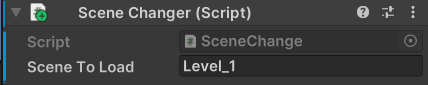
\includegraphics[width=0.6\textwidth]{images/sceneToLoad.png}
    \caption{Darstellung der SceneToLoad Variable, anhand des Level1 Buttons.}
    \label{fig:scenetoload}
\end{figure}

Für den linken Button im Hauptmenü ist beispielsweise die Spielszene \textit{Level1} vorgesehen, während für den rechten
Button die Szene \textit{Level2} zugewiesen ist. Durch diese Konfiguration im Inspector wird die Flexibilität gewährleistet,
Szenen dynamisch anzupassen, ohne dass Änderungen am eigentlichen Skript vorgenommen werden müssen. Dies ermöglicht eine
effiziente Verwaltung und Anpassung der Spielinhalte während des Entwicklungsprozesses.

\begin{lstlisting}[style=csharp, caption=Auf Knopfdruck Szene wechseln., label=code:scenechange]
using UnityEngine;
using UnityEngine.SceneManagement;

public class SceneChanger : MonoBehaviour
{
    public string sceneToLoad;

    public void ChangeScene()
    {
        if(SceneManager.GetActiveScene().name != sceneToLoad)
        {
            PlayerPrefs.DeleteAll();
            SceneManager.LoadScene(sceneToLoad, LoadSceneMode.Single);
        }
    }
}
\end{lstlisting}

Das vorliegende Skript hat eine vergleichsweise einfache Struktur. Die Variable \textbf{public string sceneToLoad} dient
als Empfänger für den Namen der zu ladenden Szene, welcher im Unity-Inspector individuell für jede Szene festgelegt werden
kann. Um den Szenenwechsel zu initiieren, wird die Methode \textbf{ChangeScene()} aufgerufen. Zunächst wird in dieser
Methode geprüft, ob die aktive Szene, die durch \textbf{SceneManager.GetActiveScene()} ermittelt wird, mit der zu ladenden
Szene übereinstimmt. Falls dies nicht der Fall ist, werden alle gespeicherten PlayerPrefabs mittels
\textbf{PlayerPrefs.DeleteAll()} gelöscht. Dieser Schritt ist von entscheidender Bedeutung, um potenzielle Komplikationen
im Zusammenhang mit dem HoloLens-Cache während des Szenenwechsels zu vermeiden.

Nachdem die Prefabs bereinigt wurden, wird die definierte Szene mit der Methode \textbf{SceneManager.LoadScene()}
geladen. Dabei wird die Ladeoption \textbf{LoadSceneMode.Single} verwendet, um sicherzustellen, dass nur die angegebene
Szene aktiv geladen wird und keine anderen Szenen im Hintergrund verbleiben. Diese präzise Steuerung des Ladevorgangs
zielt darauf ab, die Performance und Stabilität der Anwendung auf der HoloLens-Plattform zu optimieren und potenzielle
Konflikte zwischen Szeneninhalten zu vermeiden.

\subsection{UI/UX}
Die Gestaltung der Benutzeroberfläche und die damit verbundene Benutzererfahrung sind wesentliche Aspekte bei der
Konzeption und Entwicklung von Software. Eine bewährte Strategie besteht darin, sich an populären und gleichgerichteten
Anwendungen zu orientieren, insbesondere im Bereich der Augmented- oder Virtual Reality. Es wird darauf geachtet, komplexe
und verwirrende Menüstrukturen zu vermeiden und eine konsistente Farbpalette über die gesamte Benutzeroberfläche hinweg zu verwenden.

Diese Herangehensweise basiert auf der Erkenntnis, dass erfolgreiche Anwendungen in ähnlichen Domänen oft bewährte
Designprinzipien und Interaktionsmuster aufweisen, die sich positiv auf die Benutzerakzeptanz und -zufriedenheit auswirken
können. Durch die Anpassung an gängige Standards und Trends in der Branche kann das Risiko von Benutzerirritationen
und -ablehnungen minimiert werden. Gleichzeitig wird eine vertraute und angenehme Benutzererfahrung gefördert.

Es ist wichtig zu betonen, dass eine solche Inspiration von bestehenden Anwendungen nicht als direkte Kopie verstanden
werden sollte, sondern vielmehr als Quelle für Anregungen und bewährte Praktiken, die in einem eigenständigen und angepassten
Kontext implementiert werden können. Auf diese Weise kann die Effektivität und Attraktivität der Benutzeroberfläche
optimiert werden, um die Bedürfnisse und Erwartungen der Zielgruppe bestmöglich zu erfüllen.

\section{Ping Level}
In diesem Level wird das IT-Grundprinzip eines Pings zwischen zweier
PCs dargestellt. Das Kabel zwischen den zwei PCs wird von der
HoloLens getracked und mittels Kurvenberechnung wird dann eine
unsichtbare Kurve über dieses Kabel gezeichnet. Wenn dann der Benutzer
auf die Enter Taste auf einem PC drückt wird ein Ping-Paket simuliert
und auf dieser Kurve von einem PC zu dem anderen geschickt.

\subsection{Object Tracking}
Durch verwendung von bereitgestellten Technologien der HoloLens2
werden die zwei PCs und das Kabel getracked.
%Hier dann noch code zum Object Tracking einfügen

\subsection{Kurvenberechnung}
Durch Berechnung der Kurve wird das Kabel als Kurve gespeichert
und dadurch wird es ermöglicht, dass das 3D-Ping-Paket über diese
Kurve von einem PC zum anderen läuft.
%Hier dann noch code zur Kurvenberechnung einfügen

\section{Knapsack Problem Szenario}
Im zweiten Anwendungsszenario dieser Applikation liegt der Fokus auf dem bekannten Problem des Knapsack-Problems. Ziel
dieses Szenarios ist es, dieses Informatikproblem mithilfe von Augmented Reality (AR) visuell und spielerisch darzustellen.
Das Knapsack-Problem ist ein klassisches Problem der Informatik, das nicht nur an der Höheren Technischen Lehranstalt (HTL)
vermittelt wird, sondern auch von Schülern eigenständig programmiert werden soll. Dieser Ansatz dient dazu, den Anwendern
einen Einblick in die Informatik zu geben und möglicherweise Interessen für den Bereich zu wecken.

Das Unity-Anwendungsszenario für die HoloLens 2 bietet insgesamt eine interaktive und visuelle Erfahrung, bei der der
Benutzer nicht nur das Knapsack-Problem verstehen, sondern auch praktisch anwenden kann. Die Integration von AR ermöglicht
es dem Benutzer, das Problem in einer realen Umgebung zu erleben und die Optimierungsmöglichkeiten direkt zu visualisieren
und zu manipulieren. Diese immersive Herangehensweise kann dazu beitragen, das Verständnis des Knapsack-Problems zu vertiefen
und das Interesse an der Informatik zu fördern.

In diesem Abschnitt werden alle \textit{GameObjects}, \textit{Komponenten}, \textit{Scripts} und \textit{Klassen} genauer
erklärt, die in der Unity-Szene des Knapsack-Problems verwendet werden, um dieses zu realisieren.

\subsection{Knapsack-Problem Szenrio Hirarchie} \marginpar{\small\(\rightarrow\) SKREPEK}
Für einen sicheren und funktionalen Ablauf ist der Aufbau beziehungsweise die Hirarchie der Unity Szene von großer Bedeutung.
In diesem Abschnitt wird anhand der Abbildung \ref{fig:level2_hierarchy} verdeutlich wie die Unity Szene für die Implementierung
des zweiten Anwendungsszenarios für das Knapsack-Problem aufgebaut ist und es wird zusätzlich kurz darauf eingegangen
für was welches Objekt steht und welche Aufgabe dieses trägt.
\\
\begin{figure}[H]
    \centering
    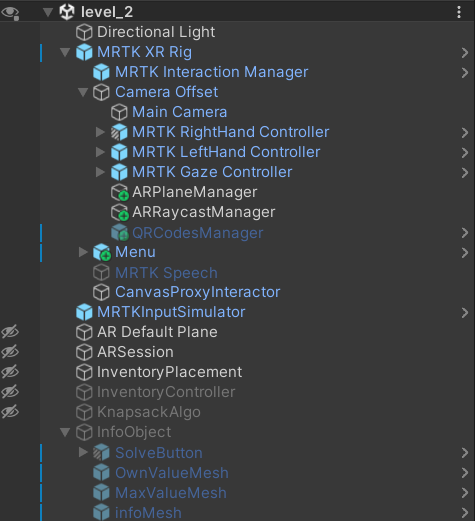
\includegraphics[scale=0.8]{images/Level2Hirarchy}
    \caption{Knapsack-Problem Szenario Hirarchie im Unity Editor.}
    \label{fig:level2_hierarchy}
\end{figure}
In dieser Abbildung ist die Hirarchie un der Inhalts des Knapsack-Problem Szenarios zu sehen. Anhand desen ist zu erkennen,
dass diese Unity Szene aus vielen wichtigen Komponenten besteht, die alle zusammenspielen, m das gewünschte Ergebnis
zu erzielen. Darunter sind folgende Objekte:
\begin{itemize}
    \item \textbf{level-2:} Ist die Unity Szene selbst, in der alle Game-Objekte enthalten sind.
    \item \textbf{MRTK XR Rig:} Grundbaustein für das Entwickeln einer XR-Applikation. Enthält wichtig Komponenten
    wie Controller für das tracken der Hände, für den User Gaze, etc.
    \item \textbf{UserInfo:} Text Objekt, dass in der \textit{main camera } liegt, damit dieses ständig im Sichtfeld des
    Benutzers liegt.
    \item \textbf{Managers:} Die drei Manager \textit{ARPlaneManager}, \textit{ARRaycastManager} und \textit{QRCodesManager}
    sind wichtiger Bestandteil um ARPlanes zu scannen, Raycasting durchzuführen und QRCodes zu erkennen.
    \item \textbf{HandMenu:} Knopf um in das Hauptmenu-Szenario zurück zu gelangen.
    \item \textbf{AR Default Plane:} Ist das Grund-Objekt für das markieren von erkannten ARPlanes.
    \item \textbf{ARSession:} Ist die Hauptkomponente, die die AR-Funktionalitäten steuert und koordiniert.
    \item \textbf{InventoryPlacementController:} Game Objekt, welches das platzieren des Inventar-Objekts handhabt.
    \item \textbf{InventoryController:} Game Objekt, welches das erkennen von neuen Objekten innerhalb des Inventar-Objekts handhabt.
    \item \textbf{KnapsackSolver:} Game Objekt, welches den Knapsack Algorithmus implementiert und das eigene Inventar berechnet.
    \item \textbf{bestSolutionPrefab:} Prefab, welches die perfekte Lösung wiederspiegelt.
    \item \textbf{InfoObject:} Dient der visualisierung von berechneten Werten und Fehlermeldungen.
\end{itemize}

In der Abbildung ist ausßredem zu sehen, dass ein Paar Game Objekte ausgegraut und nicht ausgegraut sind und, dass neben ein paar Game Objekten ein durchgestrichenes Auge zu sehen ist.
Wenn ein Game Objekt im Unity Editor ausgegraut ist bedeutet das, dass dieses GameObjekt und somit alle angehängiten Scripts von diesem Game Objekt deaktiviert sind.
Das bedeutet, dass dieses Game Objekt samt allen Scripts zu Szenenbeginn nicht aufgerufen und somit auch nicht ausgeführt werden. Nicht ausgegraute Game Objekte widerum sind
daher genau das Gegenteil. Das beudetet, dass das Game Objekt selbst samt allen angehängiten Scripts alle aktiviert sind und somit zu Szenenbeginn aufgerufen und ausgeführt werden.

Wenn neben einem Game Objekt das durchgestrichene Auge zu sehen ist bedeutet das nur, dass dieses Game Objekt im Unity Editor nicht zu sehen ist. Andererseits, wenn kein Zeichen
neben dem Game Objekt zu sehen ist, ist dieses Objekt im Unity Editor sichtbar. Dies dient dazu, dass falls in der Unity Szene viele Game Objekte vorhanden sind, dass man
diejenige ausblendet die nicht im Editor sichtbar sein müssen wie zum Beispiel Tesh Meshes oder Lables.

\subsection{Nutzung von QR-Codes} \marginpar{\small\(\rightarrow\) HAYLAZ}
Im vorherigen Abschnitt wurde bereits erwähnt, dass QR-Codes in diesem Level verwendet werden, um verschiedene Elemente
zu repräsentieren. Diese QR-Codes spielen eine entscheidende Rolle, indem sie dazu dienen, vielfältige Informationen zu
den einzelnen Objekten zu speichern und sie anschließend in einer virtuellen Umgebung abzubilden. Im folgenden Abschnitt
möchten wir näher darauf eingehen, wie genau diese QR-Codes generiert werden und welchen Zweck sie innerhalb der
Augmented Reality (AR)-Applikation erfüllen. Dabei wird insbesondere betrachtet, wie die Generierung der Codes erfolgt
und auf welche Weise sie innerhalb der Anwendung zur Interaktion mit den realen Objekten verwendet werden.

\subsubsection{Struktur und Inhalt eines QR-Codes}
Die Informationen, die in einem QR-Code gespeichert werden können, sind begrenzt. In unserem Anwendungsfall wird lediglich
eine einzelne Zahl im Bereich von 1 bis 11 abgespeichert. Diese Zahlen repräsentieren die 11 verschiedenen Modelle, die
wir unterscheiden möchten. Da nur eine Zahl gespeichert wird, genügt ein QR-Code der Größe 21x21 Module (Version 1). Die
geringe Anzahl von Modulen ermöglicht eine schnellere Erkennung, auch über größere Distanzen.
%TODO: Testen und Grafik erstellen um zu zeigen das es eine Rolle spielt welche version wir verwenden + wie groß die sind

Die zugehörigen Zahlen erhalten in der Software, genauer gesagt in der Klasse \textit{QRItem.cs}, einen Kontext. Der folgende Codeausschnitt zeigt dies:

\begin{lstlisting}[style=csharp, caption={}, label=code:update]
public class QRItem
{
    public struct QRData
    {
        public int id;
        public string name;
        public Vector3 position;
        public int weight;
        public int value;
    }

    public QRData qrData;

    public Dictionary<int, QRData> items = new Dictionary<int, QRData>()
    {
        {1, new QRData { id = 1, name = "Laptop", weight = 70, value = 100 }},
        {2, new QRData { id = 2, name = "Router", weight = 25, value = 50 }},
        {3, new QRData { id = 3, name = "Maus", weight = 20, value = 30 }},
        // ...
        {11, new QRData { id = 11, name = "Handy", weight = 30, value = 100 }}
    };

    public QRItem(int id)
    {
        items.TryGetValue(id, out qrData);
    }
}
\end{lstlisting}

In dieser Klasse wird ein Dictionary verwendet, das den Zahlen die folgenden Informationen zuordnet:

\begin{itemize}
    \item \textbf{Item Id:} Die numerische Kennung im QR-Code.
    \item \textbf{Item Name:} Die Bezeichnung des Items, das dieser QR-Code repräsentiert.
    \item \textbf{Item Position:} Die Position des Items in der virtuellen Umgebung.
    \item \textbf{Item Weight:} Das Gewicht des Items.
    \item \textbf{Item Value:} Der Wert des Items.
\end{itemize}

Diese Informationen spielen eine wesentliche Rolle in der weiteren Berechnung des Knapsack-Algorithmus.

\subsubsection{QR-Code-Tracking}
Das Tracking der QR-Codes erfolgt mithilfe des \textit{QRCodeManager.cs} Skripts. Dieses Klasse ist ein Singleton, das
die Erkennung und Verfolgung der QR-Codes steuert.

Nach der Erkennung eines QR-Codes erfolgen eine Reihe von Schritten, um diese Informationen zu speichern, verarbeiten
und zuletzt darzustellen.
Hier eine kurze Übersicht:

\begin{figure}[H]
\centering
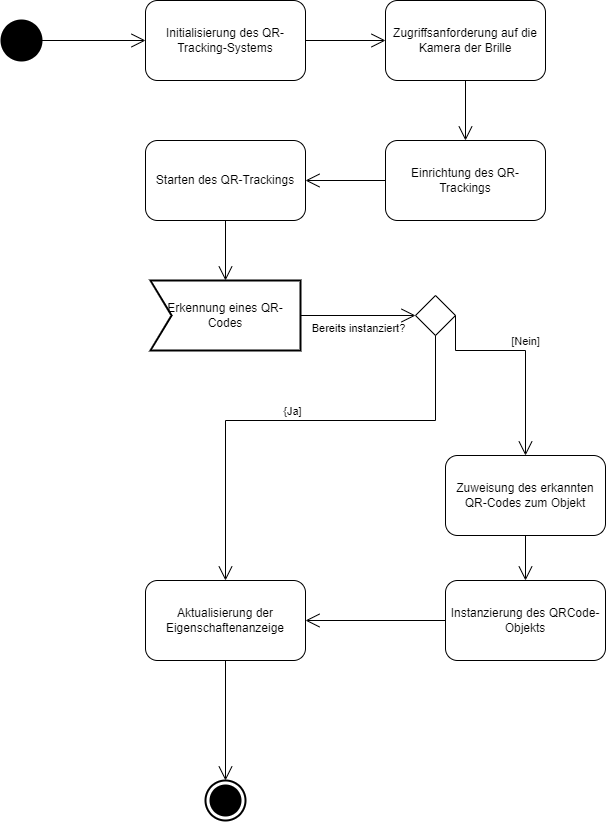
\includegraphics[scale=0.5, angle=0]{images/QRAblauf}
\caption{Ablaufdiagramm des QR-Code-Trackings.}
\label{fig:qrtracking}
\end{figure}

\begin{itemize}

\item \textbf{Initialisierung des QR-Tracking-Systems:}
Zur Aktivierung des QR-Tracking-Systems werden die erforderlichen Ressourcen und Komponenten gestartet, um die Erkennung
von QR-Codes zu ermöglichen. Dabei werden Tracking-Algorithmen gestartet, die für die Lokalisierung und Identifizierung
von QR-Codes in der Umgebung benötigt werden. Diese Initialisierung erfolgt zu Beginn der Anwendungsaktivität.

\item \textbf{Zugriffsanforderung auf die Kamera der Brille:}
%TODO: Hier Bild von "Camera acess needed" einfügen
Für das QR-Tracking wird der Zugriff auf die Kamera der Augmented-Reality-Brille benötigt. Eine Zugriffsanfrage wird
gestellt, um die notwendigen Berechtigungen zu erhalten. Dieser Schritt ist entscheidend, um visuelle Daten von der Kamera
zu erhalten und QR-Codes in der physischen Umgebung zu erkennen.

\item \textbf{Einrichtung des QR-Trackings:}
Die Einrichtung des QR-Trackings umfasst die Konfiguration von Parametern und Einstellungen, die für die korrekte
Funktion des Tracking-Systems erforderlich sind.Dazu gehören Kalibrierungsschritte, die Anpassung an die Umgebung und die
Festlegung von Erkennungsbereichen. Eine ordnungsgemäße Einrichtung gewährleistet eine zuverlässige und präzise Erkennung von QR-Codes.

\item \textbf{Starten des QR-Trackings:}
Das System sucht aktiv nach QR-Codes in der Umgebung, um sie zu erkennen. Die Kamera erfasst kontinuierlich visuelle
Daten, welche von den Tracking-Algorithmen analysiert werden, um QR-Codes zu identifizieren. Das Starten des Trackings
markiert den Beginn des fortlaufenden Erkennungsprozesses.

\item \textbf{Erkennung eines QR-Codes (Event):}
Sobald die Kamera einen QR-Code erfasst, wird dieser erkannt. Das Ereignis signalisiert, dass ein QR-Code erkannt wurde
und gibt Informationen über den erkannten QR-Code, wie seine Daten und Position, weiter.

\item \textbf{Zuweisung des erkannten QR-Codes zum Objekt:}
Nach der Erkennung wird überprüft, ob der erkannte QR-Code bereits in der Anwendung registriert ist. Falls dies der Fall
ist, wird der erkannte QR-Code einem entsprechenden Objekt in der virtuellen Umgebung zugeordnet.

\item \textbf{Instanzierung des QRCode-Objekts:}
Nach dem Scannen eines QR-Codes wird ein QR-Code-Prefab erzeugt und in der Szene platziert.

Dieses Objekt dient als Repräsentation des gescannten QR-Codes und wird als QR-Objekt bezeichnet. Es enthält visuelle
Darstellungen, Interaktionsmöglichkeiten und weitere relevante Informationen über den zugehörigen QR-Code. Die Instanziierung
ermöglicht eine nahtlose Integration des gescannten QR-Codes in die virtuelle Umgebung. Weitere Informationen zur Visualisierung
von QR-Codes finden Sie in Abschnitt \ref{sec:qr_visualization}.

\item \textbf{Aktualisierung der Eigenschaftenanzeige:}
Die Aktualisierung der Eigenschaftsanzeige dient dazu, visuelle und informative Darstellungen des erkannten QR-Codes zu
aktualisieren. Hierbei werden die Position, Größe, visuelle Darstellung und zugehörige Informationen des QR-Codes aktualisiert.
Durch die Aktualisierung wird sichergestellt, dass die Benutzer stets die neuesten Informationen über das durch den QR-Code
repräsentierte Objekt erhalten.

\end{itemize}

\subsubsection{Interaktion mit QR-Codes}
\begin{figure}[H]
\centering
\includegraphics[scale=0.5, angle=0]{images/bauklotz}
\caption{Bauklötze mit QR-Codes}
\label{fig:bauklotz}
\end{figure}
Durch die Verwendung der HoloLens können wir dem Benutzer eine visuelle Darstellung einer virtuellen Welt bieten. Um eine
Verbindung zwischen der realen und der virtuellen Welt herzustellen, nutzen wir QR-Codes.  Diese dienen als Repräsentationen
der realen Objekte, die wir in der virtuellen Welt darstellen möchten.

Wie in \ref{fig:bauklotz} zu sehen ist, sind die Bauklötze mit QR-Codes versehen. Diese Bauklötze repräsentieren die Gegenstände,
die der Benutzer in sein Inventar aufnehmen kann. Wenn der Benutzer einen Bauklotz aufhebt und ihn der HoloLens nähert, wird
der QR-Code gescannt. Dadurch werden Informationen wie das zugehörige 3D-Modell, der Wert, das Gewicht und der Name des
Gegenstands angezeigt. Auf diese Weise können wir eine nahtlose Verbindung zwischen der realen und der virtuellen Welt
herstellen und dem Benutzer eine interaktive Erfahrung bieten.

Dem Benutzer wird die Möglichkeit geboten, die Bauklötze physisch zu berühren, aufzuheben und zu fühlen. Diese sensorische
Erfahrung trägt dazu bei, die Immersion des Benutzers zu verbessern und ihm ein besseres Verständnis der virtuellen Welt
zu ermöglichen.

\subsubsection{Bestimmen der Position QR-Codes}
%TODO: Auch die events add remove und update erklären vom qrWatcher

\subsubsection{Visualisierung von QR-Codes}
%TODO: Bild von einem QR Prefab einfügen
Nachdem die genaue Platzierung der QR-Codes bestimmt wurde, steht die Aufgabe an, ihre Visualisierung in der virtuellen Welt umzusetzen.

Hierfür wird die Funktionalität von Unity Prefabs genutzt. Diese ermöglichen die Erstellung visueller Repräsentationen
der QR-Codes und ihre nahtlose Integration in die virtuelle Umgebung. Weitere Informationen zu Prefabs und ihrer Funktionsweise
finden Sie im Abschnitt \ref{Unity Prefabs}.

Innerhalb jedes Prefabs sind alle relevanten Informationen enthalten, die für die korrekte Darstellung des QR-Codes
erforderlich sind. Dazu gehören nicht nur das 3D-Modell des QR-Codes, sondern auch zugehörige Daten wie Name, Wert und
Gewicht. Diese Daten sind entscheidend für die Interaktionen innerhalb der virtuellen Umgebung.

Um die Funktionalität des QR-Codes in der virtuellen Welt zu gewährleisten, wird dem Prefab das Skript \textit{QRCodes.cs} zugewiesen.
Dieses Skript steuert die visuelle Darstellung des QR-Codes sowie sämtliche Interaktionen, die damit verbunden sind. Durch
die Zuweisung dieses Skripts wird sichergestellt, dass die QR-Codes nicht nur korrekt angezeigt, sondern auch innerhalb
der virtuellen Umgebung interaktiv sind.

%TODO: Bild von einem gescannten QRCode einfügen

\subsubsection{Zugriff auf QR-Codes bereitstellen}
Wie bereits im Abschnitt \ref{sec:KnapSackProblem} erwähnt, benötigen andere Teile der Anwendung Zugriff auf
die aktuell erkannten QR-Codes in der Szene, um entsprechend darauf reagieren zu können. Die Bereitstellung dieser Option war eine Herausforderung.
Um keine Performance-Einbußen auf der Hololens zu verursachen, läuft der Prozess des QR-Code-Trackings auf
mehreren Threads. Die aktuell erkannten QR-Codes werden in einem SortedDictionary gespeichert, welches von anderen Teilen
der Anwendung abgefragt werden kann. Da auf dieses Objekt von mehreren Threads zugegriffen wird, muss es mit einem
\textit{lock} geschützt werden, um inkonsistenzen zu vermeiden. Hierbei handelt es sich um eine Sperre, die verhindert,
dass mehrere Threads gleichzeitig auf das gleiche Objekt zugreifen. Auf diese Weise wird sichergestellt, dass die Daten
nicht inkonsistent werden und dass die Anwendung stabil und zuverlässig bleibt. Jedoch da wir Threads zugriff verweigern
müssen, um die Daten zu schützen, kann es zu einer Verzögerung kommen, bis die Daten verfügbar sind. Jedoch ist dieser
Nachteil in unserem Anwendungsfall nicht von großer Bedeutung da wir selten zur gleichen Zeit auf die Daten zugreifen und
dadurch die Verzögerung nicht bemerkbar ist.

\subsection{Inventory Placement Controller Game Objekt} \marginpar{\small\(\rightarrow\) SKREPEK}
Um eine präzise Interaktion zwischen der realen und augmentierten Realität zu gewährleisten, ist der Zugriff auf die
Kamera erforderlich, um die physische Umgebung präzise zu erfassen. Durch die Analyse der erfassten Umweltdaten können
relevante Ebenen identifiziert werden, die entscheidend sind, um eine akkurate Platzierung des Inventar-Objekts zu gewährleisten.

In diesem Abschnitt wird das \textit{Inventory Placement Controller} Game Objekt mit dem angehängten
\textit{InventoryPlacementController.cs} Script behandelt. Letzteres beinhaltet die \textbf{InventoryPlacementController}
Klasse, welche sämtliche Funktionen zur Berechnung und Platzierung des Inventars umfasst. Diese Funktionalitäten werden
im Folgenden detailliert erläutert.

\begin{figure}[H]
\centering
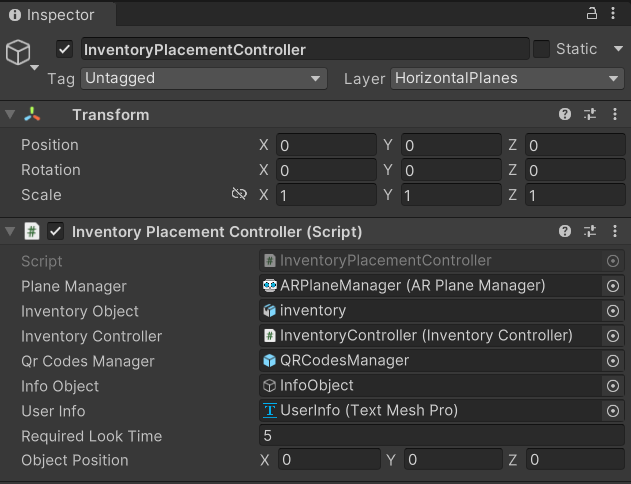
\includegraphics[scale=0.8]{images/invPlace_Editor}
\caption{inventoryPlacement Objekt im Editor}
\label{fig:inventoryPlacementController_Editor}
\end{figure}

Die Darstellung des \textit{inventoryPlacementController}-Objekts im Unity Editor, wie sie in Abbildung \ref{fig:inventoryPlacementController_Editor}
gezeigt wird, bietet eine Schnittstelle zur Konfiguration verschiedener Parameter. Hierzu zählen insbesondere die Zuweisung
der Ebenenposition, die Feinjustierung der Koordinaten innerhalb des Unity Editors sowie die Verbindung mit der Komponente
\textit{InventoryPlacementController.cs}. Zusätzlich werden voreingestellte Werte für Schlüsselvariablen angezeigt, die
für die Ausführung des Codes von entscheidender Bedeutung sind. Diese Auflistung und Erläuterung dieser Variablen umfasst:

\begin{itemize}
    \item \textbf{Plane Manager:} Hierbei handelt es sich um eine Zuweisung zum Game Objekt des \textit{ARPlanesManagers}
    aus der Szene Level 2.
    \item \textbf{Inventory Object:} Diese Referenz ist mit dem 3D-Modell des Inventars aus dem Prefab-Ordner verknüpft.
    \item \textbf{Inventory Controller:} Diese Variable ist mit dem Skript des \textit{InventoryControllers} verbunden.
    \item \textbf{QR Codes Manager:} Hierbei handelt es sich um einen Verweis auf das Game Objekt des \textit{QRCodeManagers}
    aus der Szene Level 2.
    \item \textbf{Info Object:} Diese Referenz ist mit dem Game Objekt \textit{infoObject} aus der Szene Level 2 verbunden.
    \item \textbf{User Info:} Referenz auf das TextMesh in der \textit{Main Camera}, dass zur Anzeige von Anweisungen und
    Tipps dient.
    \item \textbf{Required Look Time:} Diese Variable gibt die vorgeschriebene Zeitdauer an, für die der Benutzer auf ein
    Plane blicken muss, damit das Inventar platziert wird.
\end{itemize}

Durch den Unity Editor besteht die Möglichkeit, die Werte dieser Variablen direkt zu manipulieren, was direkte Auswirkungen
auf die Ausführung des Codes hat. Diese direkte Manipulation bietet eine intuitive und effiziente Möglichkeit, die
Einstellungen anzupassen und die Funktionalität des Programms entsprechend anzupassen.

\subsubsection{InventoryPlacementController Klassenvariablen}
\begin{lstlisting}[style=csharp, caption={Klassenvariablen der InventoryPlacementController Klasse}, label=code:anchor_var]
public ARPlaneManager planeManager;
public GameObject inventoryObject;
public InventoryController inventoryController;
public GameObject qrCodesManager;
public GameObject infoObject;
public TextMeshPro userInfo;
public float requiredLookTime = 5.0f;
public Vector3 objectPosition;

private ARPlane selectedDeskPlane;
private float lookStartTime = -1f;
private bool objectPlaced = false;
private float heightOffset = 0.001f;

private bool canStartScript = false;
\end{lstlisting}

Die dargestellten Klassenvariablen in Codeabschnitt \ref{code:anchor_var} sind integraler Bestandteil der
\textit{InventoryPlacementController} Klasse. Öffentliche (\textbf{public}) Variablen repräsentieren Objekte und Werte,
die im Unity Editor festgelegt und übergeben werden können oder von anderen Klassen für die Funktionalität benötigt werden.
Dies ermöglicht einen direkten Zugriff auf diese Objekte sowohl innerhalb der eigenen Klasse als auch von anderen Klassen
aus. Die Vektor-Variable \textit{objectPosition} spielt dabei eine entscheidende Rolle für die präzise Platzierung des
Inventar-Objekts und ebenfalls spielt das TextMesh \textit{userInfo} eine wichtige Rolle um dem Benutzer im Laufe der
Applikation Anweisung und Tips zu geben.

Hingegen dienen die privaten (\textbf{private}) Variablen der lokalen Speicherung von Werten, die ausschließlich innerhalb
der Klasse benötigt werden und von keiner anderen Klasse verwendet werden sollen.

Dieser Ansatz der Kapselung von Daten erlaubt eine klare Trennung zwischen öffentlich zugänglichen Daten und internen
Variablen, was eine effiziente und strukturierte Entwicklung und Wartung des Codes ermöglicht.
\subsubsection{Startverzögerung}
\begin{lstlisting}[style=csharp, caption={Beginn des Inventory Placement Controllers}, label=code:Start]
void Start()
{
    userInfo.text = "Schauen Sie auf einen Tisch";
    StartCoroutine(DelayedStart());
}
\end{lstlisting}
Die \textbf{Start()} Funktion wird zu Beginn des Levels für das "Knapsack-Problem" aufgerufen, wie im Codeausschnitt
\ref{code:Start} gezeigt. Diese Methode setzt den Text des \textit{userInfo} TextMeshes um den Benutzer den Ablauf anhand
einer Anweisung zu erleichtern. Zusätzlich wird die Coroutine \textbf{DelayedStart()} initiiert, die eine Verzögerung
einleitet, bevor das eigentliche Skript fortgesetzt wird.

Die Verzögerung wird gezielt eingesetzt, um dem \textit{ARPlaneManager} ausreichend Zeit zu geben, die Ebenen in der
Umgebung des Benutzers zu scannen und zu markieren. Dieser Schritt ist entscheidend, um eine stabile Grundlage für die
spätere präzise Platzierung des Inventars in der virtuellen Umgebung zu schaffen.

Die Verwendung der Coroutine ermöglicht eine zeitgesteuerte Ausführung des Codes, wodurch die Umgebungserfassung des
\textit{ARPlaneManager} abgeschlossen werden kann, bevor das Platzierungsskript aktiviert wird. Diese sorgfältig abgestimmte
Startsequenz gewährleistet eine zuverlässige Erfassung der ARPlanes und legt somit den Grundstein für eine erfolgreiche
Platzierung des Inventar-Objekts.\\

\begin{lstlisting}[style=csharp, caption={Verzoegerter Start}, label=code:DelayedStart]
private IEnumerator DelayedStart()
{
    yield return new WaitForSeconds(3.0f);
    canStartScript = true;
}
\end{lstlisting}
Die Funktion \textbf{DelayedStart()} (siehe Codeabschnitt \ref{code:DelayedStart}) wird im Kontext der \textbf{Start()}
Funktion aufgerufen, um eine initialisierte Verzögerung von 3 Sekunden zu gewährleisten, bevor das Skript seine Ausführung
fortsetzt. Diese gezielte Verzögerung ist von entscheidender Bedeutung, um dem \textit{ARPlaneManager} genügend Zeit zu
geben, um die Umgebung ungestört zu scannen. Durch die Aktivierung der Variable \textit{canStartScript} wird der Zeitpunkt
markiert, ab dem die Methode \textbf{Update()} ihre Ausführung fortsetzen kann.

\subsubsection{Identifikation des richtigen ARPlanes}
Angesichts der potenziell vielfältigen Umgebung von gescannten und markierten ARPlanes ist eine kontinuierliche Aktualisierung
erforderlich, um sicherzustellen, dass das gewünschte ARPlane stets identifiziert wird. Dieser Prozess wird durch die
Anwendung der \textbf{Update()} Funktion realisiert. Diese Methode überwacht und steuert den Auswahlvorgang des ARPlanes,
um sicherzustellen, dass das korrekte ARPlane ausgewählt wird, selbst wenn der Benutzer seinen Blick auf ein andere ARPlane
lenkt. Die dazugehörige Funktion sieht dementsprechend folgendermaßen aus:
\begin{lstlisting}[style=csharp, caption={Update Funktion}, label=code:Update]
void Update()
{
    if (!objectPlaced && canStartScript)
    {
        if (IsPointerOverPlane())
        {
            ARPlane currentPlane = GetCurrentPlaneUnderGaze();
            if (currentPlane != null)
            {
                if (selectedDeskPlane == null || selectedDeskPlane != currentPlane)
                {
                    selectedDeskPlane = currentPlane;
                    lookStartTime = Time.time;
                }
                float timeLookedAtPlane = Time.time - lookStartTime;
                userInfo.text = ((int)requiredLookTime - (int)timeLookedAtPlane).ToString();
                if (timeLookedAtPlane >= requiredLookTime)
                {
                    PlaceObjectOnDesk(selectedDeskPlane);
                    objectPlaced = true;
                    userInfo.text = "";
                }
            }
            else
            {
                selectedDeskPlane = null;
                userInfo.text = "Schauen Sie auf einen Tisch";
            }
        }
        else
        {
            selectedDeskPlane = null;
            userInfo.text = "Schauen Sie auf einen Tisch";
        }
    }
}
\end{lstlisting}
\\
Diese \textbf{Update()} Funktion wird jeden Frame der Applikation aufgerufen, um den Status des Objekts stets aktuell zu
halten. Wenn die zwei Bedingungen \textit{!objectPlaced} und \textit{canStartScript} in der \textit{Haupt if-Bedingung}
den boolschen Wert \textit{true} liefern kann das die Funktion weiter ablaufen, um das Inventar-Objekt zu platzieren.
\\
\\
Zunächst wird in der nächsten \textit{if}-Bedingung überprüft ob der Benutzer aktuell auf ein \textit{ARPlane} blickt.
Um dies zu Überprüfen wird hierzu die \textbf{IsPointerOverPlane()} aufgerufen. Der dazugehörige Code dieser Funktion:
\begin{lstlisting}[style=csharp, caption={Überprüfen ob Benutzer auf ARPlane blickt}, label=code:isPOP]
private bool IsPointerOverPlane()
{
    Ray ray = Camera.main.ScreenPointToRay(Input.mousePosition);
    RaycastHit hit;
    if (Physics.Raycast(ray, out hit))
    {
        ARPlane plane = hit.collider.GetComponent<ARPlane>();
        return (plane != null);
    }
    return false;
}
\end{lstlisting}
Die Funktion \textit{IsPointerOverPlane()} wird verwendet, um die Überprüfung der Überlagerung des Blicks des Benutzers
über einem \textit{ARPlane} zu ermöglichen.

Zunächst wird ein \textit{Ray} generiert, der ausgehend vom \textit{Hauptkameraobjekt} zur aktuellen Position des Blicks
auf dem Bildschirm erstellt wird. Dieser Vorgang wird mithilfe der Methode \textit{Camera.main.ScreenPointToRay(Input.mousePosition)}
realisiert.

\subsubsection*{Definition eines Rays} % Quelle: https://docs.unity3d.com/ScriptReference/Physics.Raycast.html
Ein Ray ist ein abstraktes Konzept in der Computergrafik und Physiksimulation, das einen unendlich langen, geraden Strahl
repräsentiert. Dieser Strahl wird durch einen Ausgangspunkt definiert, der üblicherweise als \textit{Ursprung} bezeichnet
wird. Im Kontext von dreidimensionalen Szenen und Visualisierungen entspricht der Ursprung oft der Position einer
\textit{virtuellen Kamera} oder eines \textit{Blickpunkts}.

Der Ray erstreckt sich dann in eine bestimmte Richtung, die durch Vektoren definiert wird. Diese Richtung kann durch
verschiedene Methoden festgelegt werden, abhängig von der Anwendung, in der der Ray verwendet wird. Im Falle der
Bildschirmkoordinaten kann die Richtung beispielsweise durch  Blick des Benutzers bestimmt werden.

In der Praxis wird der Ray häufig dazu verwendet, um \textit{Kollisionen mit Objekten in einer Szene zu erkennen} oder
\textit{um Lichtstrahlen für die Beleuchtungsberechnung zu simulieren}. Durch das Schießen eines Rays in eine Szene und
das Überprüfen auf \textit{Kollisionen} mit den vorhandenen Objekten kann festgestellt werden, ob der Ray ein Objekt
trifft und wenn ja, an welcher \textit{Stelle} und unter welchem \textit{Winkel}.\\

Im nächsten Schritt wird ein \textit{RaycastHit}-Objekt initialisiert, das dazu dient, relevante Informationen über
potenzielle Kollisionen zwischen dem generierten Ray und den Objekten in der Szene zu erfassen.

Anschließend wird der Ray in die Szene "geschossen", wobei währenddessen geprüft wird, ob eine Kollision mit einem Objekt
stattfindet. Sollte eine Kollision detektiert werden, werden sämtliche Details über diese Kollision in das \textit{RaycastHit}-Objekt
übertragen.

Im weiteren Verlauf wird überprüft, ob das kollidierte Objekt eine spezifische Art von Objekt repräsentiert, nämlich ein
\textit{ARPlane}. Diese Überprüfung erfolgt durch den Zugriff auf die \textit{ARPlane}-Komponente des kollidierten Objekts
mittels der Methode \textit{hit.collider.GetComponent<ARPlane>()}. Wenn diese Komponente vorhanden ist, signalisiert die
Rückgabe des Wertes \textit{true}, dass der Benutzer zum gegenwärtigen Zeitpunkt auf ein \textit{ARPlane} blickt.

Falls jedoch keine Kollision mit einem \textit{ARPlane} festgestellt wird oder das kollidierte Objekt keine
\textit{ARPlane}-Komponente aufweist, wird \textit{false} zurückgegeben. Dies deutet darauf hin, dass der Benutzer zu
diesem Zeitpunkt keinen Blick auf ein \textit{ARPlane} richtet.\\
\\
Wenn diese Funktion den boolschen Wert \textit{true} zurückliefert wird anschließend ein neues \textit{ARPlane} definiert.
Dieses ARPlane (\textit{currentPlane} wird durch den Aufruf der Funktion \textbf{GetCurrentPlaneUnderGaze()} initialisiert.
Diese Funktion sieht folgendermaßen aus:
\begin{lstlisting}[caption={Gewolltes ARPlane ermitteln}, label=code:isPOP]
private ARPlane GetCurrentPlaneUnderGaze()
{
    Ray ray = Camera.main.ScreenPointToRay(Input.mousePosition);
    RaycastHit hit;
    if (Physics.Raycast(ray, out hit))
    {
        ARPlane plane = hit.collider.GetComponent<ARPlane>();
        return plane;
    }
    return null;
}
\end{lstlisting}
Die Funktion \textbf{GetCurrentPlaneUnderGaze()} operiert auf ähnliche Weise wie die \textbf{IsPointerOverPlane()} Funktion,
jedoch mit dem entscheidenden Unterschied, dass sie ein \textit{ARPlane}-Objekt als Rückgabewert definiert. Dieser
Unterschied bezweckt, dass die Funktion das tatsächliche \textit{ARPlane}-Objekt zurückgibt, auf das der Benutzer seinen
Blick gerichtet hat.\\
\\
Nach Abschluss der beiden Funktionen \textbf{GetCurrentPlaneUnderGaze()} und \textbf{IsPointerOverPlane()} wird überprüft,
ob eine aktuelle Ebene gefunden wurde (\textit{currentPlane != null}). Wenn dies der Fall ist, wird weiterhin geprüft, ob
es sich um ein neues \textit{ARPlane} handelt oder ob es sich um dieselbe Ebene handelt, die bereits ausgewählt wurde
(\textit{selectedDeskPlane == null || selectedDeskPlane != currentPlane}). Wenn diese \textit{if}-Bedingung den boolschen
Wert \textit{true} ergibt, wird das momentan selektierte \textit{ARPlane} der Variable \textit{selectedDeskPlane} zugewiesen
und der Timer \textit{timer} wird gestartet, um aufzuzeichnen, wie lange der Benutzer auf dieses \textit{ARPlane} blickt.
Um dann abschließend noch zu visualisieren, wie lange er noch auf dieses \textit{ARPlane} blicken muss, wird der Text
des \textit{userInfos} TextMeshes auf die aktuelle Blickzeit geändert.

Abschließend wird überprüft, ob die Zeit, die der Benutzer zu dem aktuellen Zeitpunkt auf dieses spezifische \textit{ARPlane}
geblickt hat, größer oder gleich der erforderlichen Blickzeit ist (\textit{timeLookedAtPlane >= requiredLookTime}). Falls
diese Bedingung erfüllt ist, wird die Funktion \textbf{PlaceObjectOnDesk()} mit dem ausgewählten \textit{ARPlane} aufgerufen,
um das Inventar-Objekt zu platzieren. Zusätzlich wird der Status der booleschen Variable \textit{objectPlaced} auf \textit{true}
gesetzt, um zu signalisieren, dass das Inventar-Objekt platziert wurde und der Inhalt des \textit{userInfo} TextMeshes wird
geleert. Der Code für das Platzieren dieses Objekts ist wie folgt:
\begin{lstlisting}[caption={Inventar-Objekt platzieren}, label=code:placeObject]
private void PlaceObjectOnDesk(ARPlane deskPlane)
{
    qrCodesManager.SetActive(true);
    objectPosition = deskPlane.center + Vector3.up * heightOffset;
    Quaternion objectRotation = Quaternion.Euler(-90f, 0f, 0f);
    GameObject instantiatedObject = Instantiate(inventoryObject, objectPosition, objectRotation);
    instantiatedObject.transform.localScale = new Vector3(20f, 20f, 20f);
    Vector3 infoObjectPosition = objectPosition - Vector3.forward * 4.415f + Vector3.right * 0.4f;
    infoObject.transform.position = infoObjectPosition;
    infoObject.SetActive(true);
    inventoryController.SetInventoryObject(instantiatedObject);
    inventoryController.gameObject.SetActive(true);
    planeManager.planePrefab.SetActive(false);
    gameObject.SetActive(false);
}
\end{lstlisting}
Diese Funktion trägt eine tragende Rolle für den weiteren Verlauf der Applikation. Zu Beginn wird der \textit{QRCodesManager}
aktiviert um das erkennen und scannen von \textit{QRCodes} zu ermöglichen.

Als nächstes wird die Mitte des \textit{ARPlanes} berechnet um das Inventar-Objekt dementsprechend passend auf diesem zu
platzieren. Damit das Inventar-Objekt richtig rotiert ist wird dieser anschließend um \textit{90 Grad} auf der X-Achse
rotiert, dass es flach liegt. Der nächste Schritt (\textit{GameObject instantiatedObject = Instantiate(inventoryObject, objectPosition, objectRotation)})
ist dafür verantwortlich, dass das Objekt für den Benutzer sichtbar wird. Diese Funktion instanziert das Inventar-Objekt
an der definierten Position (\textit{objectPosition} und mit der definierten Rotation (\textit{objectRotation}). Zusätzlich
wird es dann noch runterskaliert. Dieselben Aktionen werden ebenfalls mit dem \textif{infoObject} vorgenommen mit dem
einzigen Unterschied, dass die Positon (\textit{infoObjectPosition}) anders berechnet wird, dass dieses neben dem Inventar-Objekt
liegt. Diese Object wird dann mittels der Funktion \textbf{.SetActive(true)} sichtbar.\\

Anschließend wird dem \textit{inventoryController} dieses Inventar-Objekt übergeben, damit dieser mit derselben Instanz
arbeitet wie der \textit{inventoryPlacementController}. Dieser wird dann ebenfalls mitels \textbf{.SetActive(true)} aktiviert.
Das Ende des \textit{inventoryControllers} stellt die Zeile \textit{gameObject.SetActive(false)} dar. Diese Zeile bewirkt,
dass das \textit{inventoryPlacementController}-GameObject selbst deaktiviert wird.\\
\\
Wenn kein aktuelles \textit{ARPlane} gefunden wird oder, wenn der Blick des Benutzers nicht auf einem \textit{ARPlane}
liegt, wird in den beiden \textit{else}-Zweigen das aktuelle ausgewählte \textit{ARPlane} auf null gesetzt, um zuvor
gespeicherte Auswahlen und davon möglich auftretende Konflikte zu vermeiden. Zusätzlich wird der Inhalt des \textit{userInfo}
TextMeshes wieder geändert, um dem Benutzer zu signalisieren, dass er wieder auf ein \textit{ARPlane} blicken muss.
\\
\\
% HIER BILD NACH PLATZIEREN DES INVENTARS EINFÜGEN
Nachdem das \textit{InventoryPlacementController} Skript ordnungsgemäß deaktiviert und beendet wurde, wird dem Benutzer
anschließend (Wie in folgender Abbildung \ref{fig:inventoryPlaced} dargestellt) Ansicht präsentiert.
\begin{figure}[H]
    \centering
    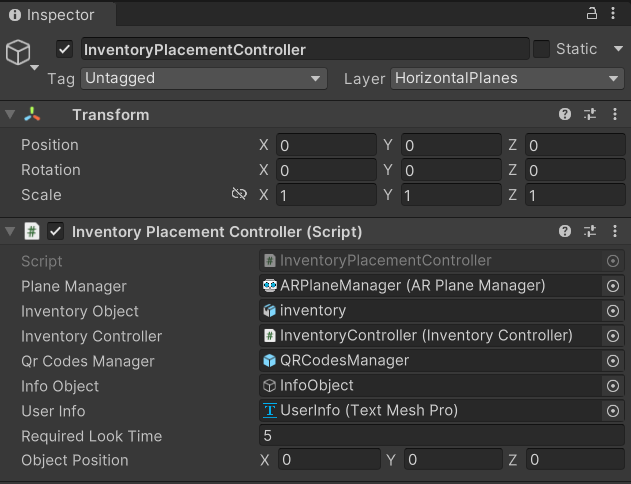
\includegraphics[scale=0.8]{images/invPlace_Editor}
    \caption{Sicht des Benutzers nach Platzierung des Inventars}
    \label{fig:inventoryPlaced}
\end{figure}

\subsection{Inventory Controller Game Objekt} \marginpar{\small\(\rightarrow\) SKREPEK}
Das \textit{Inventory Controller} Game Objekt nimmt eine essenzielle Rolle bei der Überwachung und Verwaltung des Inventars
in der Augmented Reality (AR)-Anwendung ein. Durch das angehängte Skript \textit{InventoryController.cs} wird die
\textbf{InventoryController}-Klasse implementiert. Diese Klasse ist dafür zuständig, neue Gegenstände im Inventar zu
erkennen, den verfügbaren Platz zu überprüfen, die Zellenposition anhand der QR-Code-Koordinaten zu berechnen und die
Positionen dieser Gegenstände in einem \textit{2D Array} zu speichern.

Der Zugriff auf die Begrenzungen (\textit{Bounds}) des Inventar-Modells ermöglicht eine kontinuierliche Überwachung, ob
der Benutzer ein neues Element in das Inventar gelegt hat. Dieser Ansatz gewährleistet eine präzise Kontrolle über die
Platzierung von Gegenständen im Inventar.

Das Skript \textit{InventoryController.cs} interagiert aktiv mit den AR-Elementen, insbesondere den QR-Codes, um den
Platzbedarf der Gegenstände zu überwachen und ihre Positionen im Inventar festzulegen. Zusätzlich kommuniziert der
\textit{InventoryController} auch mit dem Game Objekt \textit{KnapsackSolver}, indem er das gespeicherte \textit{2D Array}
weitergibt, um entsprechende Berechnungen durchführen zu können.

\begin{figure}[H]
    \centering
    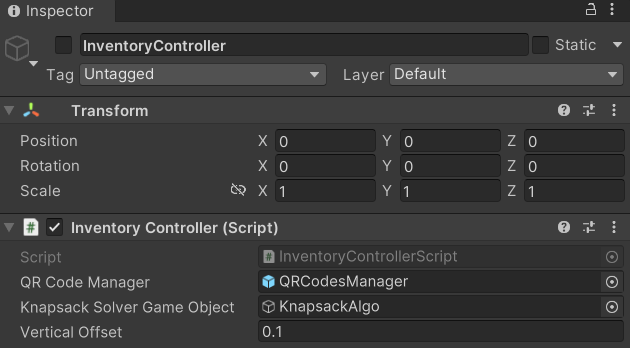
\includegraphics[scale=0.8]{images/invCon_Editor}
    \caption{InventoryController Objekt im Editor}
    \label{fig:InventoryController_Editor}
\end{figure}

Abbildung \ref{fig:InventoryController_Editor} zeigt das \textit{InventoryController}-Objekt im Unity Editor. Hier können
verschiedene Einstellungen vorgenommen werden, darunter die Ebene, in der dieses Objekt liegt, die Koordinaten im Unity
Editor und die angehängte Komponente \textit{InventoryController.cs}. Zudem sind vordefinierte Werte für bestimmte Variablen
sichtbar. Diese Variablen umfassen:

\begin{itemize}
    \item \textbf{QRCodesManager:} Referenz auf das \textit{QRCodesManager}-Game-Objekt aus der Level 2 Szene.
    \item \textbf{Knapsack Solver Game Objekt:} Referenz auf das \textit{KnapsackAlgo}-Game-Objekt aus der Level 2 Szene.
    \item \textbf{User Info:} Referenz auf das TextMesh in der \textit{Main Camera}, dass zur Anzeige von Anweisungen und
    Tipps dient.
    \item \textbf{Vertical Offset:} Float-Wert, um den die Begrenzungen (\textit{Bounds}) des Inventory-Objekts auf der
    X-Achse erweitert werden.
\end{itemize}

\subsubsection{InventoryController Klassenvariablen}
\begin{lstlisting}[style=csharp, caption={Klassenvariablen der InventoryController Klasse}, label=code:controller_var]
public GameObject QRCodeManager;
public GameObject knapsackSolverGameObject;
public TextMeshPro userInfo;

private SortedDictionary<System.Guid, GameObject> activeQRObjects;

private GameObject inventoryObject;
public float verticalOffset = 0.1f;
private Bounds inventoryBounds;
private int numRows = 3;
private int numColumns = 3;
private int[,] idGrid;
private KnapsackSolver knapsackSolver;
private int cap;
private int currWeight = 0;
private string message;
private HashSet<int> processedItems;
\end{lstlisting}\\
Die gezeigten Klassenvariablen im Codeabschnitt \ref{code:controller_var} sind Teil der \textit{InventoryController} Klasse.
Öffentliche (\textit{public}) Variablen repräsentieren Objekte und Werte, die im Unity Editor festgelegt und übergeben
werden oder von anderen Klassen für die Funktionalität benötigt werden. Dies ermöglicht einen direkten Zugriff auf diese
Objekte in der eigenen oder einer anderen Klasse. Die Float-Variable \textit{verticalOffset} spielt hier eine wichtige Rolle
für die Erweiterung der Begrenzungen (\textit{Bounds}) des Inventar-Modells und das TextMeshPro \textit{userInfo} für das
anzeigen von Anweisung und Tips für den Benutzer.

Die privaten (\textit{private}) Variablen dienen der lokalen Speicherung von Werten, die von keiner anderen Klasse benötigt
werden.

\subsubsection{Start des InventoryControllers}

Die \textbf{Start()} Funktion spielt eine Schlüsselrolle beim Initialisieren der erforderlichen Objekte und Skripte für den
erfolgreichen Start des \textit{InventoryControllers}. Diese Funktion wird zu Beginn des \textit{InventoryControllers}
aufgerufen und ist verantwortlich für die Deklaration und Einrichtung der notwendigen Komponenten. Entsprechender Code
dieser Funktion:
\begin{lstlisting}[style=csharp, caption={Start Funktion des InventoryControllers}, label=code:controller_start]
void Start()
{
    userInfo.text = "Platzieren Sie nun Gegenstände im Inventar";
    activeQRObjects = QRCodeManager.GetComponent<QRCodesVisualizer>().qrCodesObjectsList;
    knapsackSolver = knapsackSolverGameObject.GetComponent<KnapsackSolver>();
    cap = knapsackSolver.capacity;
    processedItems = new HashSet<int>();
    UpdateInventoryBounds();
    InitializeIDGrid();
}
\end{lstlisting}\\
Die Objekte, die in dieser Funktion initialisiert werden, umfassen \textit{activeQRObjects}, die für das Erkennen neuer
Objekte im Inventar entscheidend sind. Zur Weitergabe des aktualisierten Inventars im späteren Verlauf des \textit{InventoryController}
wird das \textit{KnapsackSolver}-Objekt benötigt. Zu Beginn dieser Funktion wird der Inhalt von dem \textit{userInfo}
TextMesh auf einen neuen Inhalt geändert um dem Benutzer einen Tip / eine Anweisung zu geben was, zu tun ist. Des Weiteren
werden die Kapazität (\textit{cap}) des \textit{KnapsackSolver}-Objekts gespeichert und ein \textit{processedItems-HashSet}
erstellt, um zu verfolgen, welche Objekte im Inventar bereits verarbeitet wurden. Am Ende der \textbf{Start()} Funktion
werden die beiden Funktionen \textbf{UpdateInventoryBounds()} und \textbf{InitializeGrid()} aufgerufen.

Es ist wichtig zu betonen, dass diese Funktion unmittelbar auf den vorherigen Codeabschnitt \ref{code:controller_var}
verweist, wo die relevanten Variablen der \textit{InventoryController}-Klasse definiert sind. Dies stellt sicher, dass
die Funktionalitäten, die in der \textbf{Start()} Funktion verwendet werden, korrekt initialisiert und verwendet werden
können.

\subsubsection{Bounds des Inventars aktuallisieren}
Um sicherzustellen, dass ein Item innerhalb der Grenzen des Inventars platziert werden kann, werden in der \textbf{UpdateInventoryBounds()}
Funktion einige Änderungen an dem Inventar-Objekt vorgenommen um dies zu realisieren.
\begin{lstlisting}[style=csharp, caption={Funktion um Inventar Bounds zu erweitern}, label=code:controller_updateBounds]
private void UpdateInventoryBounds()
{
    if (inventoryObject != null)
    {
        Bounds localBounds = GetBounds(inventoryObject);
        ExtendBounds(ref localBounds, verticalOffset);
        inventoryBounds = localBounds;
    }
}
\end{lstlisting}
Zunächst werden die aktuellen Begrenzungen des Inventar-Objekts gespeichert, und dann werden sie mittels der \textbf{ExtendBounds()}
Funktion erweitert. Schließlich werden diese aktualisierten Begrenzungen als neue Begrenzungen gespeichert.

Diese Funktion wird in einem größeren Kontext verwendet, insbesondere in der \textbf{Start()} Funktion des \textit{InventoryControllers},
wie in Codeabschnitt \ref{code:controller_start} zu sehen ist. Dies stellt sicher, dass die Begrenzungen des Inventars
korrekt aktualisiert werden, bevor das Inventar für den weiteren Gebrauch vorbereitet wird.


\subsubsection{Bounds des Inventars ermitteln}
Um erfolgreich auf die Begrenzungen des Inventar-Objekts zugreifen zu können, wird die Funktion \textbf{GetBounds()}
aufgerufen.

Diese Funktion ist entscheidend, da sie den \textit{Renderer} des Inventar-Modells verwendet, um die Begrenzungen zu
ermitteln. Der Renderer ist verantwortlich für die Darstellung des Modells im Spiel. Wenn der Renderer vorhanden ist
(\textit{renderer != null}), gibt die Funktion die Begrenzungen des Modells zurück. Andernfalls wird eine neue Bounds-Instanz
erstellt, die die Position des Objekts und eine Einheitsgröße hat.

\begin{lstlisting}[style=csharp, caption={Funktion um Bounds zu ermitteln}, label=code:controller_getBounds]
private Bounds GetBounds(GameObject obj)
{
    Renderer renderer = obj.GetComponent<Renderer>();
    return renderer != null ? renderer.bounds : new Bounds(obj.transform.position, Vector3.one);
}
\end{lstlisting}

Die Funktion \textbf{GetBounds()}, wie in Codeabschnitt \ref{code:controller_getBounds} dargestellt, wird von Codeabschnitt
\ref{code:controller_updateBounds} aufgerufen, um die aktuellen Begrenzungen des Inventars zu erhalten. Diese Begrenzungen
werden dann verwendet, um die Bounds des Inventars zu erweitern.

\subsubsection{Inventory Bounds erweitern}
Im weiteren Verlauf der \textbf{UpdateInventoryBounds()} Funktion, also nach dem Abschluss des Aufrufs der \textbf{GetBounds()}
Funktion, wird anschließend die Funktion \textbf{ExtendBounds()} aufgerufen (siehe Codeabschnitt \ref{code:controller_extendBounds}),
die sich darum kümmert, dass die \textit{Bounds} tatsächlich erweitert werden. Der zugehörige Code dieser Funktion:
\begin{lstlisting}[style=csharp, caption={Funktion um Bounds zu erweitern}, label=code:controller_extendBounds]
private void ExtendBounds(ref Bounds bounds, float offset)
{
    bounds.center = new Vector3(bounds.center.x, bounds.center.y + offset / 2, bounds.center.z);
    bounds.extents = new Vector3(bounds.extents.x, bounds.extents.y + offset / 2, bounds.extents.z);
}
\end{lstlisting}\\
Diese Funktion nimmt zwei Parameter an. Der erste Parameter ist eine \textit{Referenz} auf die \textit{Bounds} des
Inventar-Objekts. Die Verwendung der Referenz ermöglicht es, die Änderungen direkt an den ursprünglichen Bounds des
Inventar-Objekts vorzunehmen, was effizienter ist als die Rückgabe einer neuen Bounds-Instanz. Der zweite Parameter ist
das \textit{Offset}, um das die \textit{Bounds} des Objekts erweitert werden sollen.

Der Code der Funktion erweitert die Grenzen (\textit{Bounds}) des Inventar-Objekts um das angegebene Offset. Dies geschieht,
indem der Mittelpunkt der Bounds und ihre Ausdehnung entsprechend modifiziert werden. Die Höhe der Bounds wird um die
Hälfte des Offset-Werts erhöht, um die Bounds sowohl nach oben als auch nach unten zu erweitern, während die anderen
Dimensionen unverändert bleiben.

Nach Abschluss der \textbf{UpdateInventoryBounds()} (siehe Codeabschnitt \ref{code:controller_updateBounds}) sehen die
aktualisierten Bounds im Hintergrund dann wie auf Abbildung \ref{fig:extended_inventoryBounds} zu sehen aus.

\begin{figure}[H]
    \centering
    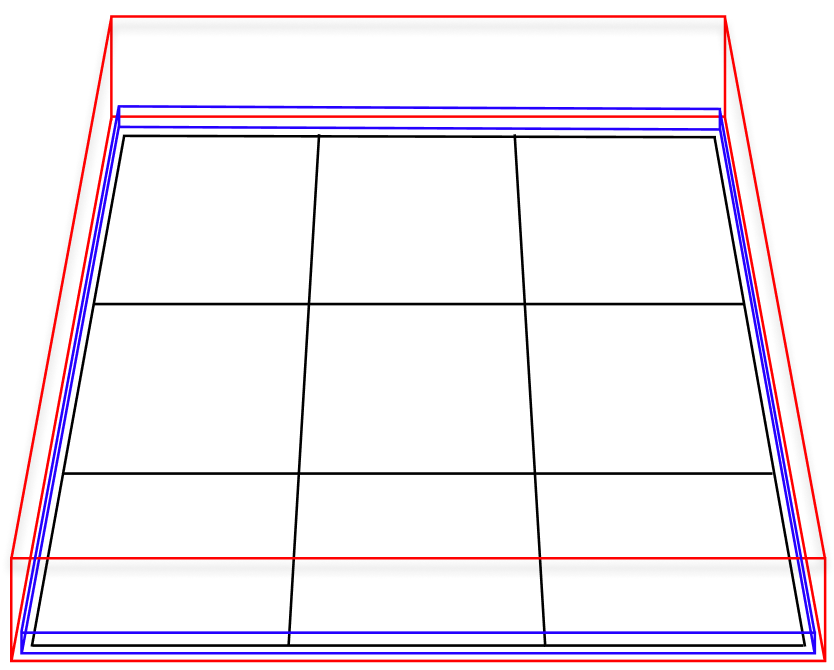
\includegraphics[scale=0.4]{images/extendedBounds}
    \caption{Erweiterte Bounds des Inventar Modells}
    \label{fig:extended_inventoryBounds}
\end{figure}

Diese Abbildung zeigt eine schematische Darstellung des zweidimensionalen Inventars. Die blaue Umrandung repräsentiert
die \textit{Bounds} des Inventar-Objekts vor der Ausführung der Funktion \textbf{UpdateInventoryBounds()}. Nach ausführung
der Funktion und erweiterung der \textit{Bounds} ist nun anhand der blauen Umrandung deutlich, dass insbesondere die
\textit{Bounds} entlang der X-Achse erweitert wurden.

Die Erweiterung der Bounds ist von entscheidender Bedeutung, da die standard \textit{Bounds} des Inventar-Objekts die
Höhe des Objekts, auf dem der QRCode befestigt ist, nicht berücksichtigen. Dies könnte dazu führen, dass ein Gegenstand,
der sich tatsächlich innerhalb der Bounds befindet, als außerhalb betrachtet wird.

Diese Anpassungen sind wichtig, um sicherzustellen, dass die Begrenzungen des Inventars korrekt erfasst werden und somit
eine präzise Verortung von QR-Codes innerhalb der Augmented-Reality-Anwendung gewährleistet ist.

\subsubsection{ID Grid Initialisierung}
Als Abschluss der \textbf{Start()} Funktion wird die \textbf{InitializeIDGrid()} Funktion die, im folgenden Codeabschnitt
\ref{code:controller_initialize} dargestellt ist, aufgerufen.
\begin{lstlisting}[style=csharp, caption={Initialisierung des idGrids}, label=code:controller_initialize]
private void InitializeIDGrid()
{
    idGrid = new int[numRows, numColumns];
}
\end{lstlisting}\\
Diese Funktion initialisiert das \textit{idGrid}, das ein zweidimensionales Array darstellt und dazu dient, die Positionen
der Gegenstände im Inventar zu speichern. Die Größe des Arrays wird durch die Variablen \textit{numRows} und \textit{numColumns}
festgelegt, die zuvor in der Klasse definiert wurden.

\subsubsection{Update-Funktion}
Um stets den aktuellen Zustand des Inventars und der darin enthaltenen \textit{Items} zu erhalten, wird hier die \textbf{Update()}
Funktion verwendet. Diese Funktion wird jeden Frame neu aufgerufen. Der zugehörige Code dazu:

\begin{lstlisting}[style=csharp, caption={Initialisierung des idGrids}, label=code:controller_update]
void Update()
{
    UpdateGrid();
}
\end{lstlisting}

\subsubsection{Neue oder entfernte Items erkennen}
Das Kernstück des \textit{InventoryController} stellt die \textbf{UpdateGrid()} dar. Diese Funktion ist hauptverantwortlich
dafür, dass neue \textit{Items} innerhalb des Inventars erkannt werden, \textit{Items} die aus dem Inventar entfernt wurden
dementsprechend entfernt werden und auch, dass bei jedem neuem oder entferntem \textit{Item} das Invetar neu berechnet
wird und darauffolgend die drei \textit{TextMeshes} innerhalb des \textit{infoObjects} aktualisiert werden, um dem Benutzer
immer  die aktuellen Inventarwerte und potentielle Fehlermeldungen anzuzeigen. Der Code zu dieser Funktion:
\begin{lstlisting}[style=csharp, caption={Neue / Entfernte Items erkennen}, label=code:controller_updateGrid]
void UpdateGrid()
{
    lock (activeQRObjects)
    {
        foreach (var item in activeQRObjects.Values)
        {
            QRCode qRCode = item.GetComponent<QRCode>();
            Vector3 worldPosition = item.transform.TransformPoint(qRCode.item.qrData.position);
            if (item != null && inventoryBounds.Contains(worldPosition))
            {
                int itemId = qRCode.item.qrData.id;
                if (!processedItems.Contains(itemId))
                {
                    if (currWeight + qRCode.item.qrData.weight <= cap)
                    {
                        userInfo.text = "";
                        processedItems.Add(itemId);
                        message = "";
                        Vector2 startGridPosition = CalculateGridPosition(worldPosition);
                        idGrid[(int)startGridPosition.x, (int)startGridPosition.y] = itemId;
                        knapsackSolver?.UpdateInfoMesh(message);
                        currWeight += qRCode.item.qrData.weight;
                        EventManager.GridUpdate(idGrid);
                    }
                    else
                    {
                        message = "Item hat zu viel Gewicht!";
                        knapsackSolver?.UpdateInfoMesh(message);
                    }
                }
            }
            else if (!inventoryBounds.Contains(worldPosition) && processedItems.Contains(qRCode.item.qrData.id) && ContainsId(qRCode.item.qrData.id))
            {
                int itemId = qRCode.item.qrData.id;
                processedItems.Remove(itemId);
                RemoveItem(itemId);
                currWeight -= qRCode.item.qrData.weight;
                EventManager.GridUpdate(idGrid);
            }
        }
    }
}
\end{lstlisting}\\
Zu Beginn der Funktion wird eine Sperre mittels einer \textit{lock}-Anweisung auf das \textit{Dictionary} der aktiven QR-Objekte
(\textit{activeQRObjects}) angewendet. Diese Maßnahme zielt darauf ab, die Datenkonsistenz zu gewährleisten, indem verhindert
wird, dass mehrere \textit{Threads} gleichzeitig auf dieses \textit{Dictionary} zugreifen und dabei gleichzeitig Änderungen
vornehmen. Ohne diese Sperre könnte es zu einem sogenannten Wettlaufzustand (\textit{race condition}) kommen, bei dem mehrere
Threads versuchen, gleichzeitig auf dasselbe Datenobjekt zuzugreifen und es möglicherweise in einen inkonsistenten Zustand
bringen könnten.

\subsubsection*{Definition einer race condition}
Ein Wettlaufzustand kann verschiedene Probleme verursachen, darunter inkonsistente oder fehlerhafte Datenoperationen. Als
Beispiel könnten Threads gleichzeitig versuchen, ein Element aus dem \textit{Dictionary} zu entfernen oder hinzuzufügen,
was zu inkonsistenten Datenzuständen führen könnte. Durch die Anwendung der \textit{lock}-Anweisung wird sichergestellt,
dass jeweils nur ein Thread gleichzeitig auf das \textit{Dictionary} zugreifen kann, wodurch potenzielle Konflikte vermieden
werden und die Datenintegrität gewährleistet ist.\\

Nachdem die Sperre angewendet wurde, durchläuft die Funktion eine \textit{foreach}-Schleife, um jedes Objekt im Dictionary
\textit{activeQRObjects} zu durchlaufen. Für jedes dieser Objekte wird die zugehörige \textit{QRCode}-Komponente mittels
der \textit{GetComponent<QRCode>()} Funktion abgerufen, um auf die spezifischen Informationen des QR-Codes zuzugreifen.
Die \textit{Weltposition} des Objekts wird anschließend berechnet, indem die \textit{lokale Position} des Objekts in
seine Weltposition umgerechnet wird.

\subsubsection*{Definition Lokale und Weltposition} %Quelle: https://medium.com/nerd-for-tech/local-space-vs-world-space-in-unity-6a9944470478#:~:text=Think%20about%20when%20you%20add,object%20related%20to%20another%20object.
In Unity bezieht sich die \textit{lokale Position} eines Objekts auf seine Position relativ zu seinem Elternobjekt oder
dem Koordinatenursprung, wenn es kein Elternobjekt hat. Diese Position wird in Bezug auf die Achsen des Objekts selbst
angegeben, unabhängig von der Umgebung.

Die \textit{Weltposition} eines Objekts ist hingegen seine Position im \textit{globalen Koordinatensystem} der Szene.
Sie berücksichtigt die Position des Objekts \textit{relativ zum Koordinatenursprung der Szene und alle Transformationen},
die auf das Objekt angewendet wurden, einschließlich der \textit{Verschiebung, Drehung und Skalierung}.

Die Berechnung der Weltposition eines Objekts erfolgt, indem seine lokale Position relativ zu seinem Elternobjekt oder zum
Koordinatenursprung in die Szene umgerechnet wird. Dies ermöglicht es, die tatsächliche Position des Objekts in der Welt
zu bestimmen und mit anderen Objekten oder Koordinaten in der Szene zu interagieren.
\begin{quote}
Angenommen, gegeben ist ein Game Objekt namens \textit{childObject}, dessen lokale Position relativ zu seinem Elternobjekt
oder zum Koordinatenursprung (0, 0, 0) wie folgt definiert ist:
\[
\text{localPosition} = (x_{\text{local}}, y_{\text{local}}, z_{\text{local}})
\]
\\
Die Weltposition des Elternobjekts (oder des Ursprungs) ist gegeben durch:
\[
\text{parentWorldPosition} = (x_{\text{parent}}, y_{\text{parent}}, z_{\text{parent}})
\]
\\
Um die Weltposition des \textit{childObjects} zu berechnen, wird stets die \textit{lokale Position} des Objekts zu der
\textit{Welt Position} seines zugehörigen Elternobjekts addiert.

\[
\text{worldPosition} = \text{parentWorldPosition} + \text{localPosition}
\]
Dies ergibt die Weltposition des childObject im globalen Koordinatensystem.
\\
\\
\textbf{Beispiel:}
Angenommen, das Elternobjekt liegt im globalen Koordinatensystem bei $(2, 0, 0)$ und die lokale Position des childObject
ist als $(0, 1, 0)$ definiert. Dann lautet die Berechnung wie folgt:

\[
\text{worldPosition} = (2, 0, 0) + (0, 1, 0) = (2, 1, 0)
\]
\\
Dies bedeutet, dass die Weltposition des \texit{childObject} im globalen Koordinatensystem (2, 1, 0) ist.\\
\end{quote}

Der folgende Schritt in der Funktion \textbf{UpdateGrid()} beinhaltet die Überprüfung der Gültigkeit des QR-Objekts
(\textit{item != null}) sowie die Feststellung, ob die berechnete Weltpositione innerhalb der definierten Begrenzungen
des Inventars liegen (\textit{inventoryBounds.Contains(worldPosition)}). Im Falle der Erfüllung dieser Bedingungen
(\textit{true}), wird das QR-Objekt weiteren Analysen unterzogen.

Zunächst wird von dem aktuellen Item die \textit{ID} mittels \textit{qRCode.item.qrData.id} gespeichert, um im weiteren
Verlauf mit dieser \textit{ID} weiterarbeiten zu können. Nach diesem Schritt wird überprüft, ob die \textit{ID} des Items
bereits in der Liste der verarbeiteten Items \textit{processedItems} enthalten ist. Wenn diese \textit{ID} neu ist und
noch nicht verarbeitet wurde, wird weiter überprüft, ob das Hinzufügen des Items die Maximale Kapazität (\textit{cap})
des Inventars überschritten wird.

Im Falle, dass das Gewicht des Items zusammen mit dem aktuellen Gesamtgewicht (\textit{currWeight}) die maximale Kapazität
(\textit{cap}) nicht überschreitet, wird der Text des \textit{infoMesh} geleert, die ID des Items zur Liste der
verarbeiteten Items (\textit{processedItems}) hinzugefügt, um es als verarbeitet zu markieren. Des Weiteren wird die Position
dieses Items innerhalb des Inventars mithilfe der Funktion \textbf{CalculateGridPosition()} berechnet und anschließend dem
\textit{idGrid} hinzugefügt. Zuletzt werden das \textit{InfoMesh} aktualisiert sowie das aktuelle Gewicht (\textit{currWeight})
und das Event \textbf{GridUpdate} des \textit{EventManagers} mit dem aktualisierten \textit{idGrid} ausgelöst. Der Code,
um die Position des Items innerhalb des Inventars zu berechnen:
\begin{lstlisting}[caption={Position des Items berechnen}, label=code:controller_calcPos, language={[Sharp]C}]
private Vector2 CalculateGridPosition(Vector3 objectPosition)
{
    float cellWidth = inventoryBounds.size.x / numColumns;
    float cellHeight = inventoryBounds.size.z / numRows;
    int col = Mathf.FloorToInt((objectPosition.x - inventoryBounds.min.x) / cellWidth);
    int row = Mathf.FloorToInt((inventoryBounds.max.z - objectPosition.z) / cellHeight);
    return new Vector2(row, col);
}
\end{lstlisting}
Die Funktion beginnt damit, die Länge einer einzelnen Zelle anhand der \textit{Bounds} in der X- und Y-Achse zu berechnen.
Die Variable \textit{cellWidth} repräsentiert die Breite jeder Zelle, während \textit{cellHeight} die Höhe jeder Zelle
im Raster des Inventars darstellt.

Anschließend werden die 2D-Koordinaten der Position des übergebenen Objekts im Raster des Inventars berechnet. Hierzu
wird die X-Koordinate des Objekts relativ zur minimalen X-Grenze der Inventar-Bounds genommen und durch die Breite einer
Zelle (\textit{cellWidth}) geteilt. Der resultierende Wert wird auf die nächstgelegene ganze Zahl abgerundet
(\textit{Mathf.FloorToInt}) und repräsentiert somit die Spalte (\textit{col}) im Raster.

Ebenso wird die Z-Koordinate des Objekts relativ zur maximalen Z-Grenze der Inventar-Bounds herbeigezogen und durch die
Höhe einer Zelle (\textit{cellHeight}) geteilt. Auch dieser Wert wird auf die nächstgelegene ganze Zahl abgerundet und
repräsentiert die Zeile (\textit{row}) im Raster.

Abschließend werden die berechneten Zeilen- und Spaltenwerte als 2D-Vektor (\textit{Vector2}) zurückgegeben. Dieser
Vektor repräsentiert die Position des Objekts im Inventar-Raster.\\
\\
Um diesen Ablauf des hinzufügen eines Gegenstandes aus der Sicht des Benutzers als auch wie dieser Prozess dann im
Hintergrund abläuft, wird hierfür ein Beispiel herangezogen.

\begin{quote}
Die visuelle Darstellung für den Benutzer, nachdem dieser einen Gegenstand in das Inventar hinzugefügt hat ist in folgender
Abbildung \ref{fig:controller_itemAdded} zu sehen.

\begin{figure}[H]
    \centering
    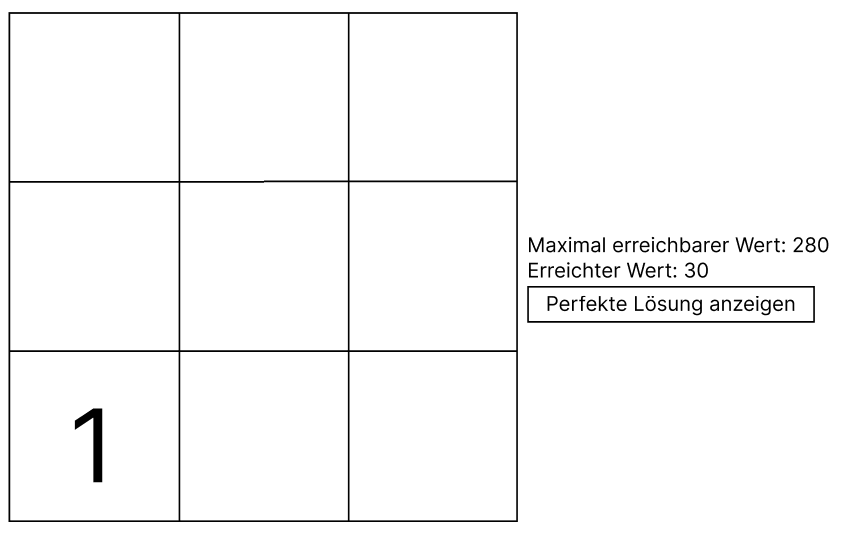
\includegraphics[scale=0.6]{images/itemAdded}
    \caption{Item zu Inventar hinzugefügt}
    \label{fig:controller_itemAdded}
\end{figure}

Auf dieser Abbilding ist zu sehen, dass in \textit{Zelle: 7} das Item mit der \textit{ID: 1} hinzugefügt wurde.

Nachdem das Item im Inventar platziert wurde, sieht das \textit{idGrid} folgendermaßen aus:
\begin{lstlisting}[style=csharp label=code:controller_savedID]
idGrid = [[0, 0, 0],
          [0, 0, 0],
          [1, 0, 0]];
\end{lstlisting}\\

Das Hashset \textit{processedItems} sieht nach dem platzieren des Items dann folgendermaßen aus:
\begin{lstlisting}[style=csharp label=code:controller_savedID]
processedItems = [1];
\end{lstlisting}\\
\end{quote}
\\
In dem anderen Fall, dass das Gewicht des Items zusammen mit dem aktuellen Gesamtgewicht (\textit{currWeight}) die maximale
Kapazität (\textit{cap}) überschreitet wird das TexMesh (\textit{InfoMesh}) mit der Nachricht, dass das Item zu schwer ist
aktualisiert.\\
\\
Um diesen Ablauf, in dem eine Vielzahl an Gegenständen in das Inventar hinzugefügt werden, wobei dar zuletzt hinzugefügte
Gegenstand zu schwer ist, wird hierfür erneut ein Beispiel herangezogen.

\begin{quote}
Der Zustand, indem der Benutzer mehrere Gegenstände zu dem Inventar hinzugefügt hat, wobei dar zuletzt hinzugefügte
Gegenstand zu schwer ist, ist in folgender Abbildung \ref{fig:controller_itemToHeavy} zu sehen. Darauf folgend ist auch
angegeben, wie dieser Ablauf im Hintergrund aussieht.

\begin{figure}[H]
    \centering
    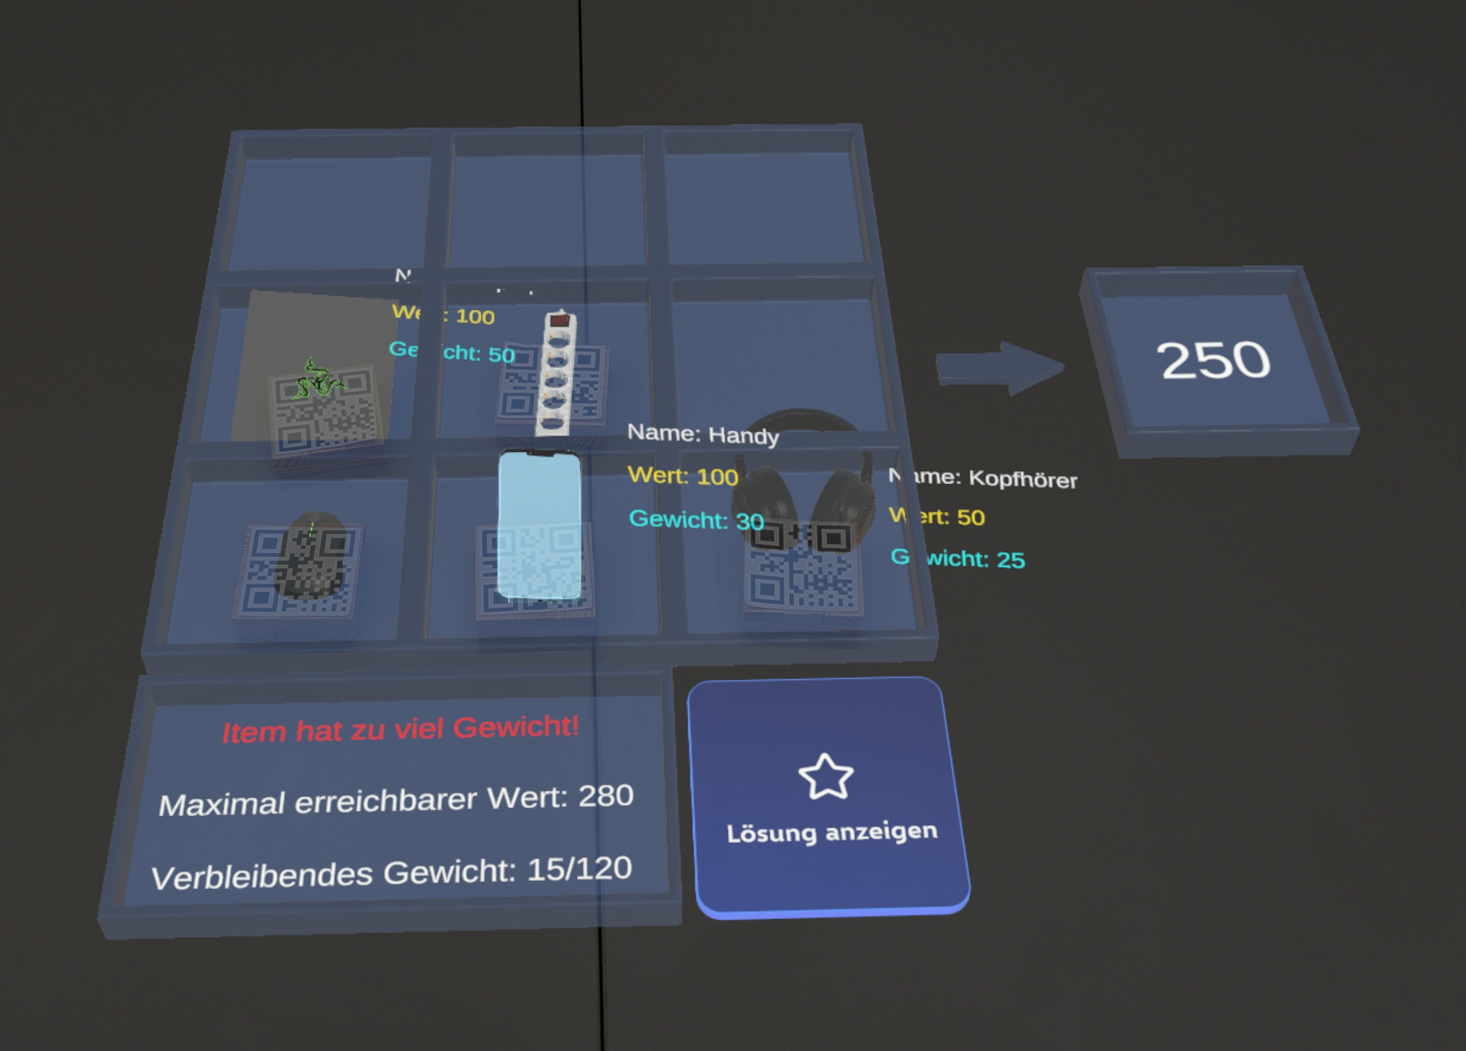
\includegraphics[scale=0.6]{images/itemToHeavy}
    \caption{Item zu schwer für das Inventar}
    \label{fig:controller_itemToHeavy}
\end{figure}

In Abbildung \ref{fig:controller_itemToHeavy} sind vier verschiedene Gegenstände im Inventar enthalten. Diese haben folgende
\textit{IDs}: 1, 3, 5, 9. Die Reihenfolge, in der diese zum Inventar hinzugefügt wurden, lautet 1, 5, 3, 9. Das Item mit der
\textit{ID: 9} wurde jedoch aufgrund seines zu hohen Gewichts nicht zu dem \textit{idGrid} und \textit{processedItems}
hinzugefügt. Gleichzeitig wird eine Fehlermeldung angezeigt, um dem Benutzer zu signalisieren, dass der zuletzt hinzugefügte
Gegenstand zu schwer für das aktuelle Inventar ist. Als Konsequenz bleiben \textit{idGrid} und \textit{processedItems}
unverändert und enthalten daher nicht die \textit{ID: 9}. Im Hintergrund sieht daher das \textit{idGrid} dementsprechend folgendermaßen aus:
\begin{lstlisting}[style=csharp label=code:controller_savedIDs]
idGrid = [[0, 0, 0],
          [5, 0, 0],
          [1, 3, 0]];
\end{lstlisting}

Das HashSet \textit{processedItems} sieht nach dem Platzieren des Items dann so aus:
\begin{lstlisting}[style=csharp, label=code:controller_savedID]
processedItems = [1, 5, 3];
\end{lstlisting}

Sobald der Benutzer dieses Item wieder aus dem Inventar entfernt, wird die Fehlermeldung nicht mehr angezeigt, und es
kann ein passendes Item hinzugefügt werden.\\
\end{quote}

Wenn sich das Item außerhalb der definierten Bounds befindet, jedoch zuvor im Inventar platziert wurde und sowohl in der
Liste der verarbeiteten Items (\textit{processedItems}) als auch im \textit{idGrid} enthalten ist, deutet dies darauf hin,
dass der Benutzer das Item aus dem Inventar entfernt hat. In diesem Fall wird die ID des Items aus der Liste der verarbeiteten
Items (\textit{processedItems}) sowie aus dem \textit{idGrid} entfernt. Zusätzlich wird das aktuelle Gesamtgewicht
(\textit{currWeight}) aktualisiert und das Event \textbf{GridUpdate} des EventManagers mit dem aktualisierten idGrid
ausgelöst. Wichtig anzumerken ist hier noch, dass in diesem \textit{else-if}-Zweig die zwei Funktionen \textbf{RemoveItem()}
und \textbf{ContainsId()} mit der aktuellen Item \textit{ID} aufgerufen werden. Der zugehörige Code der beiden Funktionen:
\begin{lstlisting}[caption={Item aus Liste entfernen}, label=code:controller_removeItem, language={[Sharp]C}]
private void RemoveItem(int id)
{
    for (int i = 0; i < numRows; i++)
    {
        for (int j = 0; j < numColumns; j++)
        {
            if (idGrid[i, j] == id)
            {
                idGrid[i, j] = 0;
                return;
            }
        }
    }
}
\end{lstlisting}

\begin{lstlisting}[caption={Überprüfen ob ID in Liste enthalten ist}, label=code:controller_checkid, language={[Sharp]C}]
private bool ContainsId(int id)
{
    for (int i = 0; i < numRows; i++)
    {
        for (int j = 0; j < numColumns; j++)
        {
            if (idGrid[i, j] == id)
            {
            return true;
        }
    }
}
return false;
}
\end{lstlisting}

Beide Funktionen operieren im Wesentlichen auf ähnliche Weise. Sie durchlaufen die Liste der verarbeiteten Items mithilfe
einer verschachtelten \textit{for-Schleife} und überprüfen, ob die als Parameter übergebene ID enthalten ist. Wenn dies
der Fall ist, wird die \textbf{RemoveItem()} Funktion die ID an dieser Stelle durch den Wert 0 ersetzen, der keinen Inhalt
repräsentiert. Die \textbf{ContainsId} Funktion hingegen überprüft lediglich, ob die ID in der Liste enthalten ist, und
gibt den boolschen Wert \textit{true} zurück, falls dies zutrifft, andernfalls \textit{false}.\\
\\
Der Fall, indem der Benutzer einen Gegenstand aus dem Inventar entfernt, wird in folgendem Beispiel veranschaulicht und
erklärt, wie dieser Ablauf im Hintergrund abläuft.

\begin{quote}
In folgender Abbildung \ref{fig:controller_itemEntfernt} ist der aktuelle Zustand eines selbst zusammengestellten Inventars
zu sehen. In diesem Inventar sind die beiden Gegenstände mit den \textit{IDs} 5 und 3 enthalten

\begin{figure}[H]
    \centering
    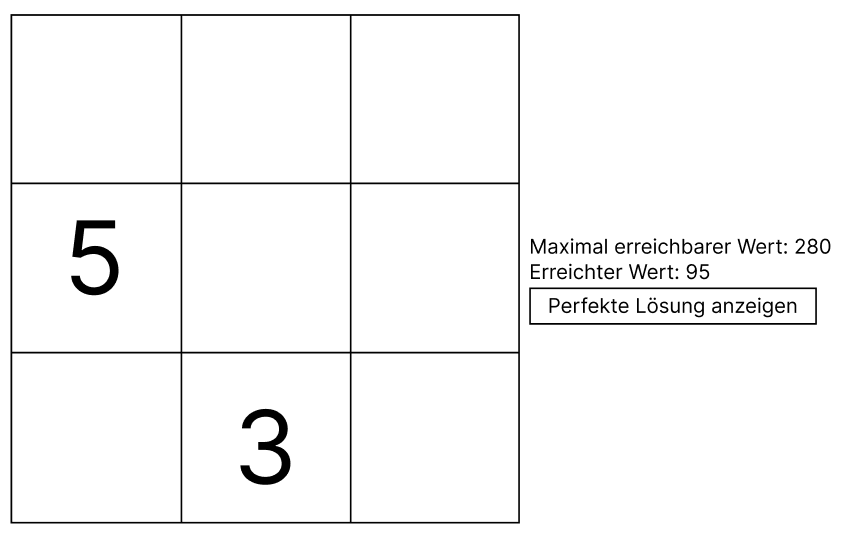
\includegraphics[scale=0.6]{images/itemEntfernt}
    \caption{Item aus Inventar entfernt}
    \label{fig:controller_itemEntfernt}
\end{figure}
Im Hintergrund sieht das \textit{idGrid} jedoch wie folgt aus:

\begin{lstlisting}[style=csharp label=code:controller_savedIDitemEntferntGrid]
idGrid = [[0, 0, 0],
          [5, 0, 0],
          [1, 3, 0]];
\end{lstlisting}

Das HashSet \textit{processedItems} sieht wie folgt aus:

\begin{lstlisting}[style=csharp label=code:controller_savedIDItemEntferntHash]
processedItems = [1, 5, 3];
\end{lstlisting}

Anhand der Abbildung \ref{fig:controller_itemEntfernt} und den gespeicherten \textit{IDs} in \textit{processedItems} und
\textit{idGrid} ist jedoch zu erkennen, dass hier noch die ID \textit{1} gespeichert ist. Dies bedeutet, dass das Item
mit der ID \textit{1} in einem früheren Zustand im Inventar platziert wurde, aber jetzt außerhalb der Grenzen des Inventars
liegt. Folglich wird diese ID aus dem \textit{idGrid} und \textit{processedItems} entfernt, und das \textit{currWeight}
wird entsprechend angepasst. Nach dem entfernen dieser ID sehen das \textit{idGrid} und das \textit{processedItems} Array
wie folgt aus:

\begin{lstlisting}[style=csharp label=code:controller_savedIDgg]
idGrid = [[0, 0, 0],
          [5, 0, 0],
          [0, 3, 0]];
\end{lstlisting}
\begin{lstlisting}[style=csharp label=code:controller_savedIDID]
processedItems = [5, 3];
\end{lstlisting}
\end{quote}


\subsection{EventManager} \marginpar{\small\(\rightarrow\) HAYLAZ}

Der \textit{EventManager} ist ein entscheidendes Game-Objekt, das als zentrales Kommunikationselement fungiert und die
Interaktion zwischen verschiedenen Komponenten und Klassen innerhalb der Anwendung ermöglicht. Implementiert als Klasse
im Skript \textit{EventManager.cs}, das dem Game-Objekt angehängt ist, spielt er eine unverzichtbare Rolle trotz seiner
Kompaktheit, da er die Schnittstelle für die Kommunikation zwischen verschiedenen Klassen und Game-Objekten bereitstellt.

Das Konzept der Ereignisse ermöglicht die Kommunikation zwischen verschiedenen Teilen eines Programms, ohne dass direkte
Abhängigkeiten zwischen diesen Teilen bestehen müssen. Andere Teile des Codes können sich auf diese Ereignisse registrieren,
um benachrichtigt zu werden, wenn sie auftreten. In diesem Zusammenhang werden spezifische Ereignisse definiert:

\begin{itemize}
\item \textbf{Nachrichteneingang}: Dieses event wird ausgelöst, wenn im ersten Level eine Nachricht von einem Laptop
empfangen wird. Nach dem Auslösen wird ein Ping-Paket über ein Kabel auf der Brille simuliert.
\item \textbf{Nachricht versendet}: Dieses Event wird ausgelöst, wenn im ersten Level eine Nachricht an einen Laptop
gesendet wird. Es dient dazu die Empfangene Nachricht an das zweite Laptop im richtigen Moment (nach Abschluss der
Simulation) weiter zu leiten.
\item \textbf{Inventar Aktualisierung}: Dieses Event wird ausgelöst, wenn im zweiten Level ein Item ins Inventar gelegt und
das Inventar aktualisiert wird. Nach der Aktualisierung wird der aktuelle Wert des Inventars berechnet. Dadurch können
wir auf eine ständige Neuberechnung des Inventars verzichten und limitierte Ressourcen sparen.
\end{itemize}

Die Klasse \textit{EventManager} definiert diese Ereignisse als statische Ereignisse und stellt Methoden bereit, um die
Ereignisse auszulösen. Dies erleichtert die globale Verwendung des Ereignissystems in verschiedenen Teilen des Codes.
Die Aktionen (Actions) sind statisch, was bedeutet, dass sie auf Klassenebene definiert sind und keine Instanz der Klasse
benötigen, um aufgerufen zu werden. Die Methode \textit{Invoke} wird verwendet, um die Ereignisse auszulösen.

\begin{lstlisting}[style=csharp, label=code:EventManager]
public static class EventManager
{
    // Level 1
    public static event System.Action<int, string, string> OnMessageReceived;
    public static void ReceiveMsg(int idx, string username, string message) => OnMessageReceived?.Invoke(idx, username, message);

    public static event System.Action<int, string, string> OnMessageSend;
    public static void SendMsg(int idx, string username, string message) => OnMessageSend?.Invoke(idx, username, message);

    // Level 2
    public static event System.Action<int[,]> OnGridUpdate;
    public static void GridUpdate(int[,] grid) => OnGridUpdate?.Invoke(grid);
}
\end{lstlisting}

Das ist die definition der Ereignisse und Methoden, die verwendet werden, um die Ereignisse auszulösen.
Um auf diese Ereignisse zu reagieren, können andere Teile des Codes sich auf diese Ereignisse registrieren, welches wie folgend
aussieht:

\begin{lstlisting}[style=csharp label=code:Event Registration]
//Dieser Code Abschnitt befindet sich in der Klasse: KnapsackSolver.cs

void Start()
{
    items = new QRItem(0).items;
    EventManager.OnGridUpdate += SetInventory;
}

public void SetInventory(int[,] newInventory)
{
    inventory = newInventory;
    CalculateKnapsack();
}
\end{lstlisting}

Nach laden der Scene registriert sich die \textit{KnapsackSolver} Klasse auf das \textit{OnGridUpdate} Event mit
der \textit{setInventory} Methode. Dies bedeutet, dass jedes mal wenn das \textit{OnGridUpdate} Event ausgelöst wird,
die \textit{setInventory} Methode aufgerufen wird und der aktuelle Wert des neuen Inventars berechnet wird.

\begin{lstlisting}[style=csharp label=code:Event Trigger]
EventManager.GridUpdate(idGrid);
\end{lstlisting}

Das auslösen des \textit{OnGridUpdate} Events wird durch den obigen Codeabschnitt erreicht. Dieser Codeabschnitt befindet
sich in der \textit{InventoryController} Klasse und wird aufgerufen, wenn ein neues Item hinzugefügt oder entfernt wird.


Insgesamt ermöglicht dieser simple Code eine lose Kopplung zwischen verschiedenen Teilen des Programms, indem Ereignisse verwendet
werden, um auf bestimmte Aktionen zu reagieren, ohne dass die beteiligten Teile voneinander wissen müssen. Dadurch wird die
Modularität, Erweiterbarkeit und Wartbarkeit der Anwendung gefördert.

\subsection{Knapsack Solver Game Objekt} \marginpar{\small\(\rightarrow\) SKREPEK}
Dieser Abschnitt befasst sich mit allem Rund um das Knapsack-Problem und auch mit dem  \textit{KnapsackSolver} GameObjekt,
welches die Hauptrolle bei der Implementierung des Knapsack Algorithmus und der Berechnung des selbst zusammengestellten
Inventars spielt. Diesem Game Objekt ist die Komponente \textit{KnapsackSolver.cs} angehängt, welches die \textit{KnapsackSolver}
Klasse realisiert.

Die \textit{KnapsackSolver} Klasse operiert in enger Zusammenarbeit mit der \textit{InventoryController} Klasse, um
sicherzustellen, dass die Berechnungen stets auf der Grundlage des aktuellen individuell zusammengestellten Inventars des
Benutzers erfolgen. Diese Interaktion gewährleistet eine präzise und aktuelle Verarbeitung der inventarbezogenen Informationen
innerhalb der Applikation.\\

\begin{figure}[H]
\centering
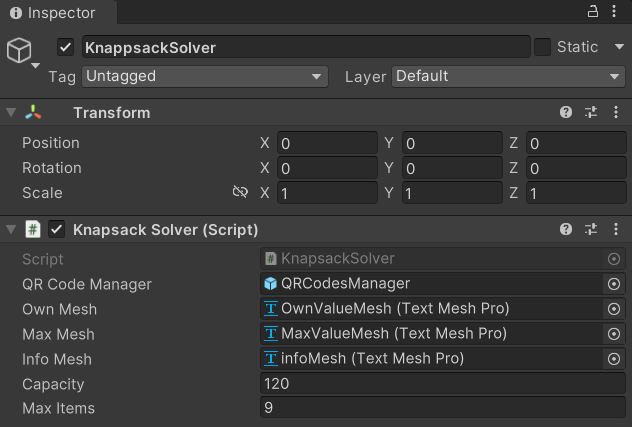
\includegraphics[scale=0.8]{images/knapsackEditor}
\caption{Knapsack Algorithmus Objekt im Editor}
\label{fig:Knapsack_Editor}
\end{figure}

Die obrige Abbildung \ref{fig:Knapsack_Editor} zeigt, dass \textit{KnapsackSolver} Game Objekt im Unity Editor. Hier können verschiedene
Einstellungen vorgenommen werden, darunter die Ebene, in der dieses Objekt liegt, die Koordinaten des Objekts im
Unity Editor selbst und die angehängte Komponente \textit{KnapsackScript.cs}. Zudem sind vordefinierte Werte für
bestimmte Variablen sichtbar. Diese Variablen umfassen:

\begin{itemize}
\item \textbf{QRCodesManager:} Referenz auf das \textit{QRCodesManager} Game Objekt aus der Level 2 Szene.
\item \textbf{Own Mesh:} Referenz auf das \textit{OwnValueMesh} aus dem \textit{infoObjekt} aus der Level 2 Szene.
\item \textbf{Max Mesh:} Referenz auf das \textit{MaxValueMesh} aus dem \textit{infoObjekt} aus der Level 2 Szene.
\item \textbf{Info Mesh:} Referenz auf das \textit{infoMesh} aus dem \textit{infoObjekt} aus der Level 2 Szene.
\item \textbf{Capacity:} Integer Wert der die Kapazität für den \textit{Knapsack Algorithmus} festlegt.
\item \textbf{Max Items:} Repräsentiert die maximale Anzahl an Items die in das Inventar gelegt werden können. Dies
dient als extra Bedingung für den \textit{Knapsack Algorithmus}.\\
\end{itemize}

\subsubsection{Knapsack-Algorithmus}
Der Knapsack-Algorithmus ist ein grundlegendes Werkzeug in der Informatik, das sich mit der optimalen Ressourcenallokation
beschäftigt, insbesondere wenn es darum geht, eine begrenzte Menge an Ressourcen effizient zu nutzen, um einen bestimmten
Nutzen oder Gewinn zu maximieren. Die Metapher des \textit{Knapsacks} bezieht sich dabei auf die Vorstellung, einen Rucksack
mit einer begrenzten Kapazität zu füllen, wobei die enthaltenen Gegenstände jeweils unterschiedliche Werte und Gewichte aufweisen.

\subsubsection{Problemstellung}
Das Knapsack-Problem befasst sich mit der Herausforderung, einen Rucksack optimal zu befüllen, wenn dieser eine begrenzte
Kapazität aufweist. Um diesen zu füllen, stehen hier eine Reihe von Gegenständen zur Auswahl, von denen jeder einen
individuellen Wert, der einen bestimmten Nutzen oder eine Wichtigkeit repräsentiert. Auch hat jeder Gegenstand ein
bestimmtes individuelles Gewicht, welches genau beschreibt, wie viel an Platz dieser Gegenstand im Rucksack einnimmt.

Das grundlegende Ziel beim Knapsack-Problem besteht darin, eine Auswahl von Gegenständen zu treffen, die in den Rucksack
passt und gleichzeitig den Gesamtwert der ausgewählten Gegenstände maximiert. Dabei muss die Summe der Gewichte der
ausgewählten Gegenstände die Kapazität des Rucksacks nicht überschreiten. Dies führt zu einer Herausforderung, bei der
eine perfekte Lösung gefunden werden muss, um den bestmöglichen Nutzen aus den verfügbaren Gegenständen zu ziehen.

\subsubsection{Variationen des Knapsack-Problems}
Im Laufe der Zeit hat das Knapsack-Problem verschiedene Variationen hervorgebracht, die jeweils unterschiedliche Aspekte
und Einschränkungen des Problems berücksichtigen. Nachfolgend werden einige bekannte Variationen erläutert.

\subsubsection*{Mehrzieliges Knapsack-Problem}
Das mehrzielige Knapsack-Problem erweitert das klassische Knapsack-Problem, indem es \textit{mehrere Zielkriterien}
berücksichtigt. Anstatt nur den Gesamtwert der ausgewählten Gegenstände zu maximieren, sollen nun mehrere Ziele \textit{gleichzeitig optimiert}
werden. Zum Beispiel könnte neben der \textit{Maximierung} des Gesamtwerts auch die \textit{Minimierung} des Gesamtgewichts
oder anderer Kosten angestrebt werden. Diese Variation des Problems führt zu komplexeren Optimierungsaufgaben, da
Kompromisse zwischen den verschiedenen Zielen gefunden werden müssen.

\subsubsection*{Multidimensionales Knapsack-Problem}
Beim multidimensionalen Knapsack-Problem hat jeder Gegenstand nicht nur ein Gewicht, sondern wird durch einen \textit{M-dimensionalen}
Vektor repräsentiert, der verschiedene \textit{Merkmale} oder \textit{Eigenschaften} des Gegenstands darstellt. Entsprechend
ist auch die Kapazität des Rucksacks ein \textit{M-dimensionaler} Vektor. Diese Variation des Problems entsteht häufig
in realen Anwendungen, in denen die Gegenstände durch mehrere Merkmale charakterisiert werden, wie zum Beispiel \texit{Größe},
\textit{Form}, \textit{Farbe} oder \textit{Material}.

\subsubsection*{Mehrere Knapsack-Probleme}
Das multiple Knapsack-Problem \textit{erweitert} das klassische Knapsack-Problem, indem es mehrere Rucksäcke oder Behälter
einführt, in die die Gegenstände verteilt werden können. Im Gegensatz zum klassischen Problem, bei dem alle Gegenstände in
einen einzelnen Rucksack gepackt werden müssen, können hier mehrere Rucksäcke genutzt werden, um die Gegenstände aufzunehmen.
Diese Variation ist relevant in Situationen, in denen die Gegenstände auf verschiedene Weise organisiert oder verwendet
werden sollen.

\subsubsection*{Quadratisches Knapsack-Problem}
Das quadratische Knapsack-Problem bezieht sich auf eine Variation, bei der das Ziel darin besteht, eine quadratische
Zielfunktion zu maximieren, die von den ausgewählten Gegenständen abhängt. Diese Zielfunktion kann beispielsweise den
Gesamtnutzen oder den Gesamtwert der ausgewählten Gegenstände darstellen und ist oft von quadratischer Form in Bezug auf
die Variablen, die die Auswahl der Gegenstände repräsentieren. Die Lösung dieses Problems erfordert spezielle Techniken
zur Bewältigung der quadratischen Struktur der Zielfunktion.

\subsubsection*{Geometrisches Knapsack-Problem}
Beim geometrischen Knapsack-Problem stehen eine Reihe von geometrischen Objekten mit unterschiedlichen \textit{Formen}
und \textit{Größen} zur Auswahl, die in einen \textit{rechteckigen Rucksack} gepackt werden sollen. Das Ziel besteht darin,
die Gegenstände so anzuordnen, dass der verfügbare Platz im Rucksack optimal genutzt wird und der Gesamtwert der
ausgewählten Gegenstände maximiert wird. Diese Variation des Knapsack-Problems erfordert eine \textit{Berücksichtigung}
der \textit{geometrischen Eigenschaften} der Objekte und kann in verschiedenen Anwendungen wie Layoutdesign oder Packungsproblemen
auftreten.\footnote{GeeksForGeeks, \cite{Introduction to Knapsack Problem, its Types and How to solve them}}

\subsubsection{Typen des Knapsack-Problems}
Das Knapsack-Problem kann in verschiedene Typen unterteilt werden, die jeweils \textit{unterschiedliche Bedingungen} und
\textit{Anforderungen} haben. Nachfolgend werden die wichtigsten Typen des Knapsack-Problems erläutert.

\subsubsection*{0/1 Knapsack-Problem}
Das 0/1-Knapsack-Problem bezieht sich auf die effiziente Auswahl von Gegenständen, um den maximalen Gesamtwert in einem
begrenzten Rucksack zu erreichen. Gegeben sind \textit{N Gegenstände}, wobei jedem Gegenstand ein bestimmtes Gewicht
(\textit{w}) und ein Wert (\textit{v}) zugeordnet ist. Außerdem steht ein Rucksack mit einer Kapazität (\textit{C}) zur
Verfügung. Das Ziel besteht darin, die Gegenstände in den Rucksack zu legen, sodass die Summe der Werte der ausgewählten
Gegenstände maximal ist.

Es ist wichtig zu beachten, dass beim 0/1-Knapsack-Problem entweder ein Gegenstand \textit{vollständig} in den Rucksack
gepackt wird oder \textit{überhaupt nicht}. Es gibt \textit{keine Möglichkeit}, einen Gegenstand \textit{teilweise} in
den Rucksack zu legen. Diese Beschränkung erfordert eine sorgfältige Auswahl der Gegenstände, um den verfügbaren Platz
im Rucksack optimal zu nutzen und gleichzeitig den Gesamtwert zu maximieren.

\subsubsection*{Fraktionales Knapsack-Problem}
Das fraktionale Knapsack-Problem befasst sich mit der effizienten Verteilung von Gegenständen in einem Rucksack, um den
Gesamtwert im Rucksack zu maximieren. Dabei werden die Gewichte und Werte von \textit{N Gegenständen} gegeben, und das
Ziel besteht darin, diese Gegenstände in einen Rucksack mit der \textit{Kapazität W} zu legen, um den maximalen Gesamtwert
zu erreichen. Im Gegensatz zum klassischen 0/1-Knapsack-Problem, bei dem entweder ein Gegenstand vollständig in den
Rucksack gepackt wird oder nicht, erlaubt das fraktionale Knapsack-Problem das Aufteilen von Gegenständen, um den Gesamtwert
im Rucksack zu maximieren. Diese Flexibilität ermöglicht es, eine perfekte Lösung zu finden, indem die Gegenstände
entsprechend ihrer Wertigkeit und Gewichtung effizient verteilt werden.

\subsubsection*{Begrenztes Knapsack-Problem}
Das begrenzte Knapsack-Problem bezieht sich auf die effiziente Auswahl von Gegenständen, um den maximalen Gesamtwert unter
Berücksichtigung eines begrenzten Gewichts zu erreichen. Angenommen, es gibt \textit{N Gegenstände}, wobei jedem Gegenstand
ein bestimmtes Gewicht (\textit{w}) und ein Wert (\textit{v}) zugeordnet ist. Die Aufgabe besteht darin, den Gesamtwert
zu maximieren, indem maximal \textit{N Gegenstände} ausgewählt werden, deren Gesamtgewicht nicht größer als das maximale
Gewicht \textit{W} ist.

\subsubsection*{Unbegrenztes Knapsack-Problem}
Das unbeschränkte Knapsack-Problem befasst sich mit der effizienten Auswahl von Gegenständen, um den maximalen Gesamtwert
zu erreichen, wobei das Gesamtgewicht nicht größer als eine vorgegebene Kapazität ist. Angenommen, es gibt ein
Rucksackgewicht \textit{W} und eine Menge von \textit{N Gegenständen}, von denen jeder einen bestimmten Wert (\textit{v})
und ein Gewicht (\textit{w}) hat. Das Ziel besteht darin, die maximale Menge zu berechnen, die genau dieses Gewicht
erreichen kann.

Im Gegensatz zum 0/1-Knapsack-Problem, bei dem die Anzahl der Instanzen eines Gegenstands begrenzt ist, können beim
unbeschränkten Knapsack-Problem \textit{beliebig viele} Instanzen \textit{desselben} Gegenstands verwendet werden. Dies
ermöglicht eine flexiblere Auswahl und Nutzung der verfügbaren Gegenstände, um den maximalen Gesamtwert zu erzielen, der
das vorgegebene Gewicht nicht überschreitet.\footnote{GeeksForGeeks, \cite{Introduction to Knapsack Problem, its Types and How to solve them}}

\subsubsection{Ansätze zur Lösung des Knapsack-Problems}
Das Knapsack-Problem bietet Raum für eine Vielzahl von Lösungsansätzen, die sich in ihrer \textit{Komplexität}, \textit{Effizienz}
und \textit{Genauigkeit} unterscheiden können. Diese Ansätze reichen von einfachen \textit{heuristischen Methoden} bis
hin zu \textit{komplexen optimierten Algorithmen}. Abgesehen von \textit{dynamischer Programmierung} und dem \textit{Greedy-Ansatz},
die später genauer betrachtet werden, gibt es weitere interessante Möglichkeiten, das Knapsack-Problem anzugehen.

Ein Ansatz besteht darin, das Problem in kleinere Teilprobleme zu zerlegen und diese dann unabhängig voneinander zu lösen.
Durch die Kombination der Lösungen dieser Teilprobleme kann eine Gesamtlösung gefunden werden. Diese Methode ist besonders
nützlich, wenn die Problemgröße groß ist und eine vollständige Suche nach einer optimalen Lösung zu aufwändig ist.

Eine weitere Herangehensweise ist die Verwendung von \textit{Metaheuristiken}, wie etwa \textit{genetische Algorithmen}
oder \textit{Schwarmintelligenz}. Diese Algorithmen basieren auf biologischen oder sozialen Konzepten und verwenden
probabilistische Techniken, um Lösungen zu finden, die möglicherweise nicht optimal, aber dennoch akzeptabel sind. Sie
eignen sich gut für komplexe Probleme, bei denen eine exakte Lösung schwer zu erreichen ist.

Eine neuere Entwicklung in der Lösung des Knapsack-Problems ist der Einsatz von \textit{maschinellem Lernen} und \textit{künstlicher Intelligenz}.
Durch den Einsatz von \textit{Datenanalyse} und \textit{statistischen Methoden} können Modelle trainiert werden, um Muster
in den Eigenschaften der Gegenstände und den Anforderungen des Rucksacks zu erkennen und optimale Packstrategien vorherzusagen.

\subsubsection*{Dynamischer Programmieransatz genauer betrachtet}
Der dynamische Programmieransatz ist eine leistungsfähige Methode zur Lösung des Knapsack-Problems, die auf der Idee beruht,
das Problem in kleinere Teilprobleme zu zerlegen und die Lösungen dieser Teilprobleme systematisch zu kombinieren, um die
optimale Gesamtlösung zu finden. Diese Methode eignet sich besonders gut für Probleme, bei denen Teilprobleme sich überlappen
und dieselben Teillösungen verwendet werden können, um mehrere Teilprobleme zu lösen.

Der folgende Pseudocode veranschaulicht den dynamischen Algorithmus zur Lösung des Knapsack-Problems:
\begin{lstlisting}[style=csharp, caption={Dynamischer Algorithmus}]
FUNCTION knapsackDynamic(weights[], values[], capacity)
    n = length(weights)
    DECLARE Tabelle[n + 1][capacity + 1]
    FOR i FROM 0 TO n DO
        FOR w FROM 0 TO capacity DO
            IF i == 0 OR w == 0 THEN
                Tabelle[i][w] = 0
            ELSE IF weights[i-1] <= w THEN
                Tabelle[i][w] = MAX(values[i-1] + Tabelle[i-1][w - weights[i-1]], Tabelle[i-1][w])
            ELSE
                Tabelle[i][w] = Tabelle[i-1][w]
            END IF
        END FOR
    END FOR
    RETURN Tabelle[n][capacity]
END FUNCTION
\end{lstlisting}\\
\\
Die Funktion \textbf{knapsackDynamic} implementiert den dynamischen Programmieransatz zur Lösung des Knapsack-Problems.
Sie akzeptiert drei Parameter: ein Array von Gewichten (\( \textit{weights} \)), ein Array von Werten (\( \textit{values} \))
und die Kapazität des Rucksacks (\( \textit{capacity} \)).

Zuerst wird die Länge des Gewichtsarrays \( \textit{n} \) berechnet, um die Anzahl der verfügbaren Gegenstände zu bestimmen.
Dann wird eine Tabelle \( \textit{Tabelle} \) mit \( \textit{n+1} \) Zeilen und \( \textit{capacity+1} \) Spalten initialisiert.
Diese Tabelle dient dazu, die optimalen Werte für verschiedene Teilprobleme zu speichern.

Anschließend werden zwei verschachtelte Schleifen verwendet, um alle möglichen Kombinationen von Gegenständen und Gewichten
zu durchlaufen. Dabei wird für jedes Teilproblem in der Tabelle der optimale Wert berechnet. Die innere Schleife iteriert
über die möglichen Kapazitäten des Rucksacks, während die äußere Schleife die verfügbaren Gegenstände durchläuft.

Für jedes Teilproblem wird überprüft, ob der aktuelle Gegenstand in den Rucksack passt. Wenn ja, wird der Wert dieses
Gegenstands zu dem Wert addiert, der erreicht werden kann, wenn der Rucksack ohne diesen Gegenstand gefüllt wird. Andernfalls
wird der Wert aus der vorherigen Zeile der Tabelle übernommen, da der aktuelle Gegenstand nicht in den Rucksack passt.

Schließlich wird der Wert in der untersten rechten Zelle der Tabelle zurückgegeben, der den maximal erreichbaren Gesamtwert
des Rucksacks darstellt.

Dieser Algorithmus nutzt die Eigenschaften der optimalen Teilstruktur und des Überlappungsprinzips aus, um eine effiziente
Lösung des Knapsack-Problems zu finden. Durch die systematische Berechnung und Speicherung der optimalen Werte für Teilprobleme
ermöglicht der dynamische Programmieransatz eine Zeitkomplexität von \( O(n \cdot capacity) \), was für viele praktische
Anwendungen akzeptabel ist.


\subsubsection*{Aufbau und Interpretation der Tabelle der Teilprobleme}
Die Tabelle der Teilprobleme spielt eine entscheidende Rolle bei der systematischen Lösung des Knapsack-Problems mithilfe
des dynamischen Programmieransatzes. Sie ist eine zweidimensionale Matrix, die während des Algorithmusverlaufs generiert
wird und die optimalen Lösungen für verschiedene Teilprobleme des Knapsack-Problems enthält. Die Matrix ist wie folgt strukturiert:

\[
\left[
\begin{array}{ccccc}
a_{11} & a_{12} & a_{13} & \cdots & a_{1n} \\
a_{21} & a_{22} & a_{23} & \cdots & a_{2n} \\
a_{31} & a_{32} & a_{33} & \cdots & a_{3n} \\
a_{31} & a_{32} & a_{33} & \cdots & a_{3n} \\
\vdots & \vdots & \vdots & \ddots & \vdots \\
a_{m1} & a_{m2} & a_{m3} & \cdots & a_{mn} \\
\end{array}
\right]
\]

Jede \textit{Zeile} in der Matrix entspricht den verschiedenen verfügbaren Gewichtskapazitäten des Rucksacks, beginnend
bei \textit{null} und schrittweise bis zur \textit{maximalen Kapazität}.

Jede \textit{Spalte} in der Matrix repräsentiert die Anzahl der bereits \textit{berücksichtigten Gegenstände}, wobei jede
Spalte die \textit{Teilprobleme} für eine zunehmende Anzahl von Gegenständen darstellt.\\
\\
Um anschließend eine Zelle \( a_{mn} \) dieser Matrix zu interpretieren, ist Folgendes wichtig zu wissen:
\begin{enumerate}
\item \textbf{m} gibt an, wie viel \textit{Gewicht} bereits im Rucksack verbraucht wurde. Je weiter fortgeschritten dieser
Wert ist, daher desto weiter unten in der Tabelle und desto mehr Gewicht wurde bereits verwendet.
\item \textbf{n} gibt an, wie viele \textit{Gegenstände} bereits betrachtet wurden. Je weiter fortgeschritten, daher,
desto weiter rechts in der Tabelle und desto mehr Gegenstände wurden bereits berücksichtigt.
\end{enumerate}

Die Einträge in der Matrix werden durch den \textit{dynamischen Programmieransatz} berechnet, indem die optimalen Werte für
Teilprobleme \textit{schrittweise kombiniert} werden, um den Wert für größere Teilprobleme zu bestimmen.

\subsubsection*{Greedy-Ansatz genauer betrachtet}
Im Gegensatz zur dynamischen Lösung wählt der Greedy-Ansatz Gegenstände basierend auf bestimmten Kriterien aus, um eine
lokale Optimierung zu erreichen. Hierbei wird in jedem Schritt diejenige Entscheidung getroffen, die im Moment am
vorteilhaftesten erscheint, ohne jedoch die Gesamtoptimierung im Auge zu behalten.

Der folgende Pseudocode veranschaulicht den Greedy-Algorithmus zur Lösung des Knapsack-Problems:

\begin{lstlisting}[style=csharp, caption={Greedy Algorithmus}]
FUNCTION knapsackGreedy(weights[], values[], capacity)
    n = length(weights)
    DECLARE items[n]
    FOR i FROM 0 TO n DO
        items[i] = (values[i] / weights[i], weights[i], values[i])
    END FOR
    SORT items by ratio in descending order
    totalValue = 0
    currentWeight = 0
    FOR i FROM 0 TO n DO
        IF currentWeight + items[i].weight <= capacity THEN
            currentWeight += items[i].weight
            totalValue += items[i].value
        ELSE
            ratio = (capacity - currentWeight) / items[i].weight
            totalValue += ratio * items[i].value
            BREAK
        END IF
    END FOR
    RETURN totalValue
END FUNCTION
\end{lstlisting}\\
Die Funktion \textbf{knapsackGreedy()} nimmt wie der dynamische Ansatz drei Parameter an: ein Array von Gewichten (\( \textit{weights} \)),
ein Array von Werten (\( \textit{values} \)) und die Kapazität des Rucksacks (\( \textit{capacity} \)). Die Funktionsweise
dieses Ansatzes ist wie folgt:

\begin{enumerate}
    \item Zunächst wird für jeden Gegenstand das Verhältnis von Wert zu Gewicht berechnet und in einer Liste von Tupeln
    gespeichert. Jedes Tupel enthält das Wert-Gewichts-Verhältnis sowie das Gewicht und den Wert des entsprechenden Gegenstands.
    \item Die Liste der Gegenstände wird basierend auf dem Verhältnis von Wert zu Gewicht in absteigender Reihenfolge
    sortiert, um die Gegenstände mit dem höchsten Verhältnis zuerst zu betrachten.
    \item Der Algorithmus durchläuft die sortierte Liste der Gegenstände und versucht, jeden Gegenstand dem Rucksack
    hinzuzufügen. Dabei wird überprüft, ob das Hinzufügen des Gegenstands das Gewichtslimit des Rucksacks überschreitet.
    Falls dies der Fall ist, wird ein Teil des Gegenstands entsprechend dem verbleibenden verfügbaren Gewicht im Rucksack hinzugefügt.
    \item Nachdem alle Gegenstände überprüft wurden, wird der Gesamtwert der im Rucksack enthaltenen Gegenstände zurückgegeben.
    Dies stellt die Lösung des Problems dar.
\end{enumerate}

Der Greedy-Algorithmus bietet eine einfache und effiziente Lösung für das Knapsack-Problem, die jedoch nicht immer die
perfekte Lösung garantiert. Durch die Auswahl der Gegenstände basierend auf lokalen Kriterien kann der Algorithmus zu
suboptimalen Ergebnissen führen, insbesondere wenn die Gegenstände stark voneinander abhängen oder das Gewichtslimit des
Rucksacks sehr restriktiv ist.

\subsubsection{Anwendungen des Knapsack-Problems}
Die grundlegende Problemstellung des Knapsack-Problems hat breite Anwendung in verschiedenen \textit{wissenschaftlichen}
und \textit{industriellen} Bereichen gefunden und bildet die Grundlage für eine Vielzahl von Algorithmen und Anwendungen.

Dieses Kapitel untersucht die Anwendungen des Knapsack-Problems und seine Bedeutung in verschiedenen Domänen. Von der
\textit{Logistik} über die \textit{Finanzplanung} bis hin zum \textit{Ressourcenmanagement} und der \textit{Netzwerkoptimierung}
hat das Knapsack-Problem einen entscheidenden Einfluss auf die moderne Technologie und Wirtschaft.

Die Anwendungen des Knapsack-Problems lassen sich in vier Hauptbereiche unterteilen:
\begin{enumerate}
    \item \textbf{Logistik}: Der Knapsack-Algorithmus wird in der Logistik angewendet, um den Transport von Gütern mit
    begrenzten Kapazitäten zu optimieren. Indem er die bestmögliche Auswahl von Gütern trifft, ermöglicht er Logistikunternehmen,
    ihre Transportkosten zu minimieren und die Effizienz ihrer Lieferketten zu steigern. Dies kann die Planung von LKW-Routen,
    die Beladung von Containern oder die Organisation von Waren in Lagern umfassen.
    \item \textbf{Finanzplanung}: In der Finanzplanung wird der Knapsack-Algorithmus genutzt, um Portfolios von Investitionen
    zu optimieren. Investoren können mithilfe dieses Algorithmus eine Auswahl von Wertpapieren treffen, die das Risiko
    minimieren und den erwarteten Ertrag maximieren. Dies kann die Diversifizierung von Anlagen, die Auswahl von Aktien
    oder die Verwaltung von Fonds umfassen.
    \item \textbf{Ressourcenmanagement}: Der Knapsack-Algorithmus wird im Ressourcenmanagement verwendet, um die effiziente
    Nutzung begrenzter Ressourcen sicherzustellen. Dies kann in der Produktion erfolgen, wo Arbeitskräfte, Maschinen und
    Materialien effizient zugewiesen werden müssen, oder im Projektmanagement, um Zeit und Budgets zu optimieren. Durch
    die Anwendung des Knapsack-Problems können Unternehmen ihre Produktivität steigern und Kosten senken.
    \item \textbf{Netzwerkoptimierung}: In der Netzwerkoptimierung spielt der Knapsack-Algorithmus eine wichtige Rolle
    bei der Planung und Optimierung von verschiedenen Arten von Netzwerken. Dies kann die Optimierung von Transportrouten,
    die Verteilung von Ressourcen in Computernetzwerken oder die Verbesserung der Bandbreitenauslastung in Telekommunikationsnetzen
    umfassen. Der Einsatz des Knapsack-Problems ermöglicht es, die Leistung von Netzwerken zu verbessern und Engpässe zu
    minimieren.\footnote{GeeksForGeeks, \cite{Introduction to Knapsack Problem, its Types and How to solve them}}
\end{enumerate}

Die Untersuchung dieser Anwendungen veranschaulicht die Vielseitigkeit und Effektivität des Knapsack-Problems bei der Lösung
komplexer Optimierungsprobleme. Darüber hinaus trägt die Anwendung des Knapsack-Algorithmus dazu bei, industrielle Abläufe
zu verbessern, Kosten zu senken und die Effizienz in verschiedenen Bereichen zu steigern.

\subsubsection{Auswahl des Implementierungsansatzes}
Die Wahl des Implementierungsansatzes für den Knapsack-Algorithmus in dieser Anwendung ist von entscheidender Bedeutung
für den Erfolg des Projekts. Moderne Softwaresysteme stehen vor einer Vielzahl von Herausforderungen und Anforderungen,
die eine sorgfältige Auswahl eines geeigneten Algorithmus erforderlich machen.

Die Entscheidung für den Implementierungsansatz erfolgte nach einer eingehenden Analyse der Anforderungen der Anwendung
und einer gründlichen Untersuchung der verfügbaren Algorithmen sowie ihrer Eigenschaften. Dabei wurden verschiedene
Faktoren berücksichtigt, darunter die Notwendigkeit einer optimalen Lösung, die Effizienz der Algorithmusausführung, die
Flexibilität in Bezug auf unterschiedliche Problemvarianten und die Genauigkeit der berechneten Ergebnisse.

Diese überlegungen werden anschließend ausführlich diskutiert und die Gründe für die Wahl des dynamischen Ansatzes als
Implementierungsstragie für den Knapsack-Algorithmus erläutert:
\begin{enumerate}
    \item \textbf{Perfekte Lösungsgarantie}: Der dynamische Ansatz bietet die Möglichkeit, eine perfekte Lösung für das
    Knapsack-Problem zu garantieren. Dies ist besonders wichtig in Anwendungen, in denen eine genaue und zuverlässige
    Lösung erforderlich ist, um optimale Entscheidungen zu treffen.
    \item \textbf{Effizienz}: Obwohl der dynamische Ansatz im Vergleich zum Greedy-Ansatz einen höheren Rechenaufwand
    erfordert, bietet er dennoch eine effiziente Lösung für das Knapsack-Problem. Durch die Verwendung von dynamischer
    Programmierung können Teilprobleme effizient gelöst und die Gesamtlösung optimiert werden.
    \item \textbf{Flexibilität}: Der dynamische Ansatz ist flexibel und kann auf verschiedene Varianten des Knapsack-Problems
    angewendet werden, einschließlich 0/1-Knapsack, unbeschränktem Knapsack und anderen Typen. Dadurch ist er vielseitig
    einsetzbar und kann an die spezifischen Anforderungen einer Anwendung angepasst werden.
    \item \textbf{Genauigkeit}: Durch die Verwendung des dynamischen Ansatzes können exakte Werte für den maximal erreichbaren
    Wert des Rucksacks und die optimale Auswahl von Gegenständen berechnet werden. Dies ermöglicht eine präzise Bewertung
    und Planung basierend auf den berechneten Ergebnissen.
\end{enumerate}

In Anbetracht dieser Überlegungen wurde der dynamische Ansatz als die geeignete Methode zur Implementierung des Knapsack-Algorithmus
in dieser Applikation gewählt. Seine Fähigkeit, eine perfekte Lösung zu garantieren, kombiniert mit seiner Effizienz und
Flexibilität, macht ihn zu einer idealen Wahl für die Behandlung des Knapsack-Problems in diesem Kontext.

\subsubsection{KnapsackSolver Klassenvariablen}
\begin{lstlisting}[style=csharp, caption={Klassenvariablen des KnapsackSolvers}, label=code:Klassenvariablen_kn]
public GameObject QRCodeManager;
public TextMeshPro ownMesh;
public TextMeshPro maxMesh;
public TextMeshPro infoMesh;

public int[,] usedItems;
public int capacity = 120;
public Dictionary<int, QRData> items;
public int maxItems = 9;

private int[,] inventory;
\end{lstlisting}\\
\\
Die im Codeabschnitt \ref{code:Klassenvariablen_kn} gezeigten Klassenvariablen gehören zur \textit{KnapsackSolver}-Klasse.
Diese Variablen werden verwendet, um Objekte und Werte innerhalb des Unity Editors zu repräsentieren, die entweder direkt
festgelegt und übergeben werden oder von anderen Klassen aus Funktionalitätsgründen benötigt werden. Die öffentlichen
(\textit{public}) Variablen ermöglichen einen direkten Zugriff auf diese Objekte in der eigenen oder einer anderen Klasse.

Das \textit{2D int Array inventory} spielt eine entscheidende Rolle im Verlauf des \textit{KnapsackSolvers}, da es verwendet
wird, um das individuell vom Benutzer zusammengestellte Inventar zu verarbeiten und zu berechnen.

Die privaten (\textit{private}) Klassenvariablen dienen hauptsächlich dem lokalen Speichern von Werten, die nur innerhalb
der \textit{KnapsackSolver}-Klasse benötigt werden und keinen Zugriff von außen erfordern.

\subsubsection{Start des KnapsackSolvers}
Die \textbf{Start()} Funktion, die in folgendem Codeabschnitt \ref{code:kn_start} abgebildet ist, ist der Startpunkt d
es \textit{KnapsackSolvers}.

\begin{lstlisting}[style=csharp, caption={Klassenvariablen der InventoryController Klasse}, label=code:kn_start]
void Start()
{
    items = new QRItem(0).items;
    EventManager.OnGridUpdate += SetInventory;
}
\end{lstlisting}\\
\\
Zu Beginn der Funktion wird dem Dictionary \textit{items} ein neues Objekt des Typs \textit{QRitem} zugewisen, wobei die
\textit{ID} 0 übergeben wird. Dies ermöglicht den Zugriff auf das Dictionary in der \textit{QRItem} Klasse welches alle
Daten der einzelnen Items enthält. Anschließend wird das Event \textit{OnGridUpdate} des \textit{EventManagers} ausgelöst
und die Funktion \textbf{SetInventory()} aufgerufen. Letztere ist eine Rückruffunktion, die als Reaktion auf das Ereignis
aufgerufen wird und die Aufgabe hat, das Inventar zu aktualisieren. Diese Funktion sieht wie folgt aus:
\begin{lstlisting}[style=csharp, caption={Inventar setzen}, label=code:kn_start]
public void SetInventory(int[,] newInventory)
{
    inventory = newInventory;
    CalculateKnapsack();
}
\end{lstlisting}

\subsubsection{Starten der Berechnung}
Um stets mit dem aktuellen Inventar zu rechnen, wird bei jedem mal, bei dem die \textbf{SetInventory()} Funktion
aufgerufen wird, das aktuelle Inventar (\textit{inventory}) mit dem neuen Inventar in dem ein neues Item enthalten ist
(\textit{newInventory}) aktualisiert. Um anschließend die tatsächlichen Werte zu berechnen, wird die \textbf{CalculateKnapsack()}
Funktion aufgerufen. Der Code zu dieser Funktion:
\begin{lstlisting}[style=csharp, caption={Berechnungsfunktion}, label=code:kn_calc]
void CalculateKnapsack()
{
    int maxValue = KnapsackMaxValue(out usedItems);
    int inventoryValue = -1;
    maxMesh.text = "Maximal erreichbarer Wert: " + maxValue.ToString();
    try
    {
        inventoryValue = KnapsackInventoryValue(inventory);
        if (maxValue == inventoryValue)
        {
            infoMesh.color = Color.green;
            infoMesh.text = "Maximale Punktzahl erreicht";
        }
        else
        {
            infoMesh.text = "";
        }
        ownMesh.text = "Erreichter Wert: " + inventoryValue.ToString();
    }
    catch (Exception e)
    {
        Debug.LogError("Error calculating inventory value: " + e.Message);
    }
}
\end{lstlisting}\\
\\
Die Funktion \textbf{CalculateKnapsack()} startet den Algorithmus zur Berechnung des Knapsackproblems. Zunächst wird eine
Variable \textit{maxValue} initialisiert, welche den maximal erreichbaren Wert des Rucksacks repräsentiert. Diese wird
durch den Aufruf der Funktion \textbf{KnapsackMaxValue()} initialisiert, wobei auch eine Liste von \textit{usedItems}
als Ausgabe zurückgegeben wird. Diese Liste repräsentiert die in der \textit{perfekten Lösung} enthaltenen Items.

Anschließend wird die Variable \textit{inventoryValue} initialisiert und auf -1 gesetzt, um in dem Fall eines Fehlers
keinen Programm-Crash zu verursachen. Die Funktion \textbf{KnapsackMaxValue()} wird anhand eines \textit{try-catch} Blocks
versucht auszuführen, wobei der Wert des aktuellen Inventars als Argument übergeben wird. Falls dieser Wert erfolgreich
berechnet wird, wird er der Variable \textbf{inventoryValue} zugewiesen.

Nach der Berechnung des maximal erreichbaren Werts (\textit{maxValue}) des Rucksacks wird geprüft, ob dieser Wert mit dem
Wert des aktuellen Inventars (\textit{inventoryValue}) übereinstimmt. Eine solche Übereinstimmung deutet darauf hin, dass
der Benutzer eine perfekte Lösung gefunden hat. Diese Optimalität wird visuell durch die Farbänderung des \textit{infoMesh}
auf Grün und die Anzeige einer entsprechenden Erfolgsmeldung verdeutlicht. Im Gegensatz dazu wird bei Abweichungen zwischen
dem maximal erreichbaren Wert und dem Wert des aktuellen Inventars der Text des \textit{infoMesh} gelöscht, um vorherige
Meldungen zu entfernen und das Feedbackfeld zu bereinigen.

Nachdem der Wert des zusammengestellten Inventars berechnet wurde, wird dieser im \textit{ownMesh} angezeigt. Sollte während
dieser Berechnung ein Fehler auftreten, wird eine entsprechende Fehlermeldung in die \textit{Log-Datei} geschrieben, um
die Fehlerbehandlung und -verfolgung zu unterstützen.\\
\\
Um den beschriebenen Zustand der Erreichung einer perfekten Lösung zu verdeutlichen, wird im Folgenden ein Beispiel herangezogen.

\begin{quote}
Wie der beschriebene Ablauf, des findens einer perfekten Lösung aussieht, ist in folgender Abbildung \ref{fig:foundperfsol}
zu sehen.
\begin{figure}[H]
\centering
\includegraphics[scale=0.6]{images/foundperfsol}
\caption{Sicht des Benutzers nach finden einer perfekten Lösung}
\label{fig:foundperfsol}
\end{figure}

% TODO: Bild machen mit perfekten Lösung und in folgendem Text IDs einfügen
Auf dieser Abbildung ist zu sehen, dass das Inventar mit den Gegenständen mit folgenden \textit{IDs}: ., .,. ,. ,. befüllt
ist und der errechnete Wert dieses Inventars dem der perfekten Lösung gleicht. Diese Erkenntnis ist anhand des \textit{infoMesh}
zu erkennen in dem eine Erfolgsnachricht in grüner Farbe dargestellt ist.
\end{quote}

\subsubsection{Knapsack-Algorithmus Implementierung}
Dieser Abschnitt behandelt die Implementierung der allgemeinen Variation des 0/1 Knapsack-Problems anhand des dynamischen
Algorithmus zur Lösung des Knapsack-Problems. Die Implementierung erfolgt in der Funktion \textbf{KnapsackMaxValue()}.
Diese Funktion gibt ein zweidimensionales Array zurück, das eine perfekte Lösung für das Problem speichert. Die Funktion
besteht im Wesentlichen aus zwei wichtigen Abschnitten:

Der erste Abschnitt beinhaltet die Implementierung des Algorithmus selbst, während der zweite Abschnitt dazu dient, die
ausgewählten Gegenstände zu verfolgen, die zur Erreichung des maximalen Werts verwendet wurden. Anhand dieser Gegenstände
wird dann das Array \textit{usedItems} erstellt, welches die perfekte Lösung repräsentiert.

Im Folgenden wird der Code dieser Funktion präsentiert:
\begin{lstlisting}[style=csharp, caption={Knapsack Algorithmus / Item Backtracking}, label=code:startKnapsack]
public int KnapsackMaxValue(out int[,] usedItems)
{
    int n = items.Count;
    int[,] dp = new int[n + 1, capacity + 1];
    bool[,] selected = new bool[n + 1, capacity + 1];
    for (int i = 0; i <= n; i++)
    {
        for (int w = 0; w <= capacity; w++)
        {
            if (i == 0 || w == 0)
                dp[i, w] = 0;
            else if (i <= maxItems && items[i].weight <= w)
            {
                int newValue = items[i].value + dp[i - 1, w - items[i].weight];
                if (newValue > dp[i - 1, w])
                {
                    dp[i, w] = newValue;
                    selected[i, w] = true;
                }
                else
                {
                    dp[i, w] = dp[i - 1, w];
                    selected[i, w] = false;
                }
            }
            else
            {
                dp[i, w] = dp[i - 1, w];
                selected[i, w] = false;
            }
        }
    }
    int[,] tempUsedItems = new int[3, 3];
    int row = n;
    int col = capacity;
    int rowIndex = 0;
    int colIndex = 0;
    while (row > 0 && col > 0 && rowIndex < 3 && colIndex < 3)
    {
        if (selected[row, col] && colIndex < maxItems)
        {
            tempUsedItems[rowIndex, colIndex] = items[row].id;
            col -= items[row].weight;
            row--;
            colIndex++;
            if (colIndex >= 3)
            {
                colIndex = 0;
                rowIndex++;
            }
        }
        else
        {
            row--;
        }
    }
    usedItems = tempUsedItems;
    return dp[n, capacity];
}
\end{lstlisting}
Die Implementierung des Knapsack-Algorithmus in den Zeilen drei bis 32 der Funktion \textbf{KnapsackMaxValue()} dieses
Abschnitts entspricht im Wesentlichen dem bereits erklärten Pseudocode. Ein wesentlicher Unterschied besteht jedoch darin,
dass diese spezielle Implementierung eine zusätzliche Bedingung berücksichtigt. Diese Bedingung besagt, dass zur Berechnung
des maximalen Werts und damit der optimalen Lösung maximal 9 Gegenstände in die Berechnung miteinbezogen werden können.
Dies ist darauf zurückzuführen, dass im vorliegenden Inventar-Objekt nur 9 verfügbare Zellen vorhanden sind, in die ein
Gegenstand eingefügt werden kann. Die Erfüllung dieser Bedingung wird in dem
\textit{else-if}-Zweig $i \leq \text{maxItems} \land \text{items}[i].\text{weight} \leq w$ gewährleistet.

Zusätzlich wird ein Array von booleschen Werten namens \textit{selected} erstellt, um im Verlauf der Berechnung diejenigen
Gegenstände zu markieren, die ausgewählt wurden (\textit{selected = true}). Dieses Array wird verwendet, um im zweiten
Teil der Funktion die perfekte Lösung zusammenzustellen.\\

Der zweite Teil dieses Codes, der sich um das \textit{Backtracking} der in der perfekten Lösung verwendeten Items kümmert,
beginnt damit, dass Variablen initialisiert werden, um den aktuellen Zeilen- und Spaltenindex in dem \textit{selected}
Array zu verfolgen, sowie \textit{Indezes} für das temporäre Array, die die ausgewählten Gegenstände speichert. Zunächst
wird eine Schleife gestartet, um durch das \textit{selected} Array
zu iterieren und die ausgewählten Gegenstände zu identifizieren.

Während der Iteration werden Bedingungen überprüft, um zu entscheiden, ob ein Gegenstand ausgewählt wurde. Wenn ein
Gegenstand ausgewählt wird, wird seine \textit{ID} in das temporäre Array (\textit{tempUsedItems})eingefügt, und die
Position in der Tabelle wird aktualisiert, indem das Gewicht des ausgewählten Gegenstands von der aktuellen Kapazität
subtrahiert wird. Die Schleife durchläuft die Tabelle und fährt fort, bis entweder die erste Zeile oder Spalte erreicht
wird oder die maximal zulässige Anzahl von ausgewählten Gegenständen erreicht ist.

Wenn ein Gegenstand ausgewählt wird, wird seine ID in die temporäre Matrix eingefügt, um die ausgewählten Gegenstände zu
speichern. Die Indizes der temporären Matrix werden aktualisiert, um den nächsten verfügbaren Speicherplatz zu zeigen.
Andernfalls wird der Zeilenindex dekrementiert, um zur vorherigen Zeile in des \textit{selected} Arrays zu gehen.

Am Ende der Funktion wird der Wert von \textit{usedItems} mit dem ermittelten Array \textit{tempUsedItems} überschrieben
und der maximale Wert des Rucksacks wird zurückgegeben.
\subsubsection*{Aufbau und Interpretation der selected Tabelle}
Angenommen, es sind die folgenden  5 Gegenstände (indiziert von 1 bis 5) mit den folgenden Werten und Gewichten gegeben:
\[
\begin{array}{|c|c|c|}
\hline
\text{Gegenstand} & \text{Wert} & \text{Gewicht} \\
\hline
1 & 10 & 5 \\
\hline
2 & 6 & 4 \\
\hline
3 & 8 & 3 \\
\hline
4 & 3 & 2 \\
\hline
5 & 7 & 1 \\
\hline
\end{array}
\]
\\
Und die \textit{Kapazität} des Rucksacks liegt bei 5. Aufgrund dieser Angaben wird die \textit{selected}-Matrix nach
Ausführung des Knapsack-Algorithmus basierend auf den ausgewählten Gegenständen gefüllt. Diese Matrix sieht dann folgendermaßen
aus:

\[
\begin{array}{|c|c|c|c|c|c|}
\hline
& 0 & 1 & 2 & 3 & 4 \\
\hline
0 & \text{false} & \text{false} & \text{false} & \text{false} & \text{false} \\
\hline
1 & \text{false} & \text{false} & \text{false} & \text{false} & \text{true} \\
\hline
2 & \text{false} & \text{false} & \text{false} & \text{true} & \text{true} \\
\hline
3 & \text{false} & \text{false} & \text{true} & \text{true} & \text{true} \\
\hline
4 & \text{false} & \text{true} & \text{true} & \text{true} & \text{true} \\
\hline
5 & \text{false} & \text{true} & \text{true} & \text{true} & \text{true} \\
\hline
\end{array}
\]
Für die Interpretation der \textit{selected}-Matrix ist es wichtig zu verstehen, wie sie funktioniert. Jede Zelle in dieser
Matrix gibt an, ob der entsprechende Gegenstand in der perfekten Lösung des Knapsack-Problems enthalten ist (\textit{true})
oder nicht (\textit{false}). Als Beispiel zeigt die Zelle $selected[4][3]$, dass der Gegenstand 4 in der perfekten Lösung
miteinbezogen wurde, als die Kapazität des Rucksacks 3 betrug. Diese Informationen ermöglichen folgende Schlussfolgerungen:
\begin{enumerate}
    \item Der Index \textbf{i} in $selected[i][j]$ repräsentiert den Gegenstand, der in Betracht gezogen wird.
    \item Der Index \textbf{j} in $selected[i][j]$ gibt die Kapazität des Rucksacks an, die für diese Teillösung verwendet
    wurde.
\end{enumerate}

\subsubsection{Berechnung des eigenen Inventars}
Die letzte Berechnugn die in dem \textit{KnapsackSolver} durchgeführt wird, ist die Berechnung des eigenen Inventars. Dies
wird mittels der \textbf{KnapsackInventoryValue()} Funktion erreicht. Der Code dieser Funktion:
\begin{lstlisting}[style=csharp, caption={Funktion um eigenes Inventar zu brechnen}]
public int KnapsackInventoryValue(int[,] inventory)
    {
    if (inventory == null)
    {
        throw new System.Exception("Inventory is null");
    }
    int totalValue = 0;
    foreach (var item in items.Values)
    {
        int itemId = item.id;
        int itemValue = item.value;
        for (int j = 0; j < inventory.GetLength(0); j++)
        {
            for (int k = 0; k < inventory.GetLength(1); k++)
            {
                if (inventory[j, k] == itemId)
                {
                    totalValue += itemValue;
                }
            }
        }
    }
    return totalValue;
}
\end{lstlisting}
In dieser Funktion wird der Gesamtwert des aktuellen Inventars berechnet, welches durch das zweidimensionales Array
(\textit{inventory}) repräsentiert wird. Zunächst wird überprüft, ob das übergebene Inventar korrekt gesetzt wurde und
ob es \textit{null} ist oder nicht. Falls es \textit{null} ist, wird eine \textit{Exception} geworfen. Falls das Inventar
nicht leer ist, wird die Variable \textit{totalValue} initialisiert, um den Gesamtwert des Inventars zu speichern.
Anschließend wird eine \textit{foreach}-Schleife über jedes Element des Dictionaries \textit{items} durchgeführt, wobei
die \textit{ID} und der Wert \textit{value} jedes Elements ermittelt und in \textit{itemId} und \textit{itemValue}
gespeichert werden.

Anschließend werden zwei verschachtelte \textit{for}-Schleifen verwendet, um jedes Element im \textit{inventory}-Array
zu durchlaufen. Wenn die \textit{ID} des Gegenstands im \textit{inventory}-Array gefunden wird, wird der Wert dieses
Gegenstands zum Gesamtwert \textit{totalValue} addiert. Nach Abschluss der beiden \textit{for}-Schleifen wird dieser
ert schließlich zurückgegeben.

\subsubsection{InfoMesh aktualisieren}
Der \textit{KnapsackSolver} enthält zwei Funktionen, die sowohl in der Klasse selbst als auch in der
\textit{InventoryController} Klasse gebraucht werden. Die Funktion \textbf{SetInventory()} wurde bereits erklärt und
die zweite Funktion ist die folgende:

\begin{lstlisting}[style=csharp, caption={Funktion um InfoMesh zu verändern}]
public void UpdateInfoMesh(string input)
{
    infoMesh.color = Color.red;
    infoMesh.text = input;
}
\end{lstlisting}
Diese Funktion wird von der Klasse \textit{InventoryController} verwendet und sie dient dazu, das \textit{infoMesh} mit
einem neuen Text zu aktualisieren und rot zu färben, um dem Benutzer Fehler anzuzeigen.

\subsection{Best Solution Prefab Game Objekt} \marginpar{\small\(\rightarrow\) SKREPEK}
Das \textit{best solution prefab} nimmt eine zentrale Rolle im weiteren Verlauf der Applikation ein. Mittels des angefügten
\textit{PerfectSolutionVisualizer.cs} Skripts wird die \textbf{PerfectSolutionVisualizer} Klasse implementiert, die die
Visualisierung der zuvor berechneten optimalen Lösung ermöglicht. Diese Visualisierung ist von entscheidender Bedeutung,
um dem Benutzer die bestmögliche Lösung aufzuzeigen, ihr Erscheinungsbild zu veranschaulichen und die enthaltenen Elemente
dieser Lösung deutlich zu machen.
\begin{figure}[H]
    \centering
    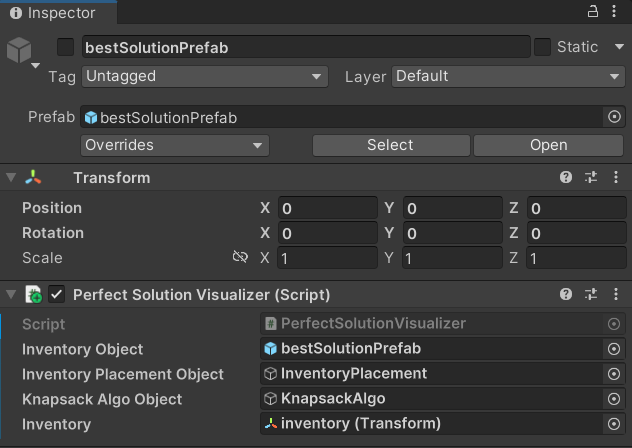
\includegraphics[scale=0.8]{images/bestSolPref_Editor}
    \caption{bestSolutionPrefab im Unity Editor}
    \label{fig:bestSol_Editor}
\end{figure}

In Abbildung \ref{fig:bestSol_Editor} ist das \textit{bestSolutionPrefab} im Unity Editor dargestellt. Hier können
verschiedene Einstellungen vorgenommen werden, darunter die Ebene, in der dieses Objekt platziert ist, die Koordinaten
des Objekts im Unity Editor selbst sowie die angehängte Komponente \textit{PerfectSolutionVisualizer.cs}. Des Weiteren
sind vordefinierte Werte für bestimmte Variablen sichtbar. Diese Variablen umfassen:
\begin{itemize}
    \item \textbf{Inventory Object:} Eine Referenz auf das \textit{Prefab} für die perfekte Lösung.
    \item \textbf{Inventory Placement Object:} Eine Referenz auf das \textit{inventoryPlacement} Game Objekt.
    \item \textbf{Knapsack Algo Object:} Eine Referenz auf das \textit{KnapsackSolver} Game Objekt.
    \item \textbf{Inventory:} Eine Referenz auf das \textit{Inventory} Modell, das im Best Solution Prefab enthalten ist.
\end{itemize}

\begin{figure}[H]
    \centering
    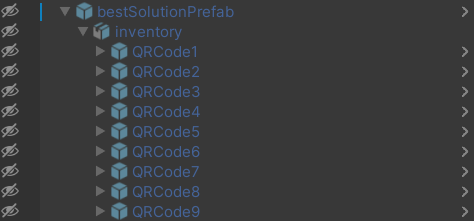
\includegraphics[scale=0.8]{images/bestSolPref}
    \caption{Inventar Prefab Hirarchie im Unity Editor}
    \label{fig:InvPref}
\end{figure}

Abbildung \ref{fig:InvPref} zeigt die Struktur des Prefabs für die perfekte Lösung. Hierbei ist zu erkennen, dass das
Haupt-Game-Objekt das Game-Objekt \textit{Inventory} enthält. Dieses \textit{Inventory}-Game-Objekt repräsentiert das
3D-Modell des Inventars. Des Weiteren hat dieses \textit{Inventory}-Game-Objekt mehrere untergeordnete Prefabs. Diese
\textit{QRItem}-Prefabs sind entscheidend, um basierend auf der ID das entsprechende Modell anzuzeigen. Die Gesamtstruktur
des Prefabs sieht dann im Unity-Editor wie folgt aus:
\begin{figure}[H]
    \centering
    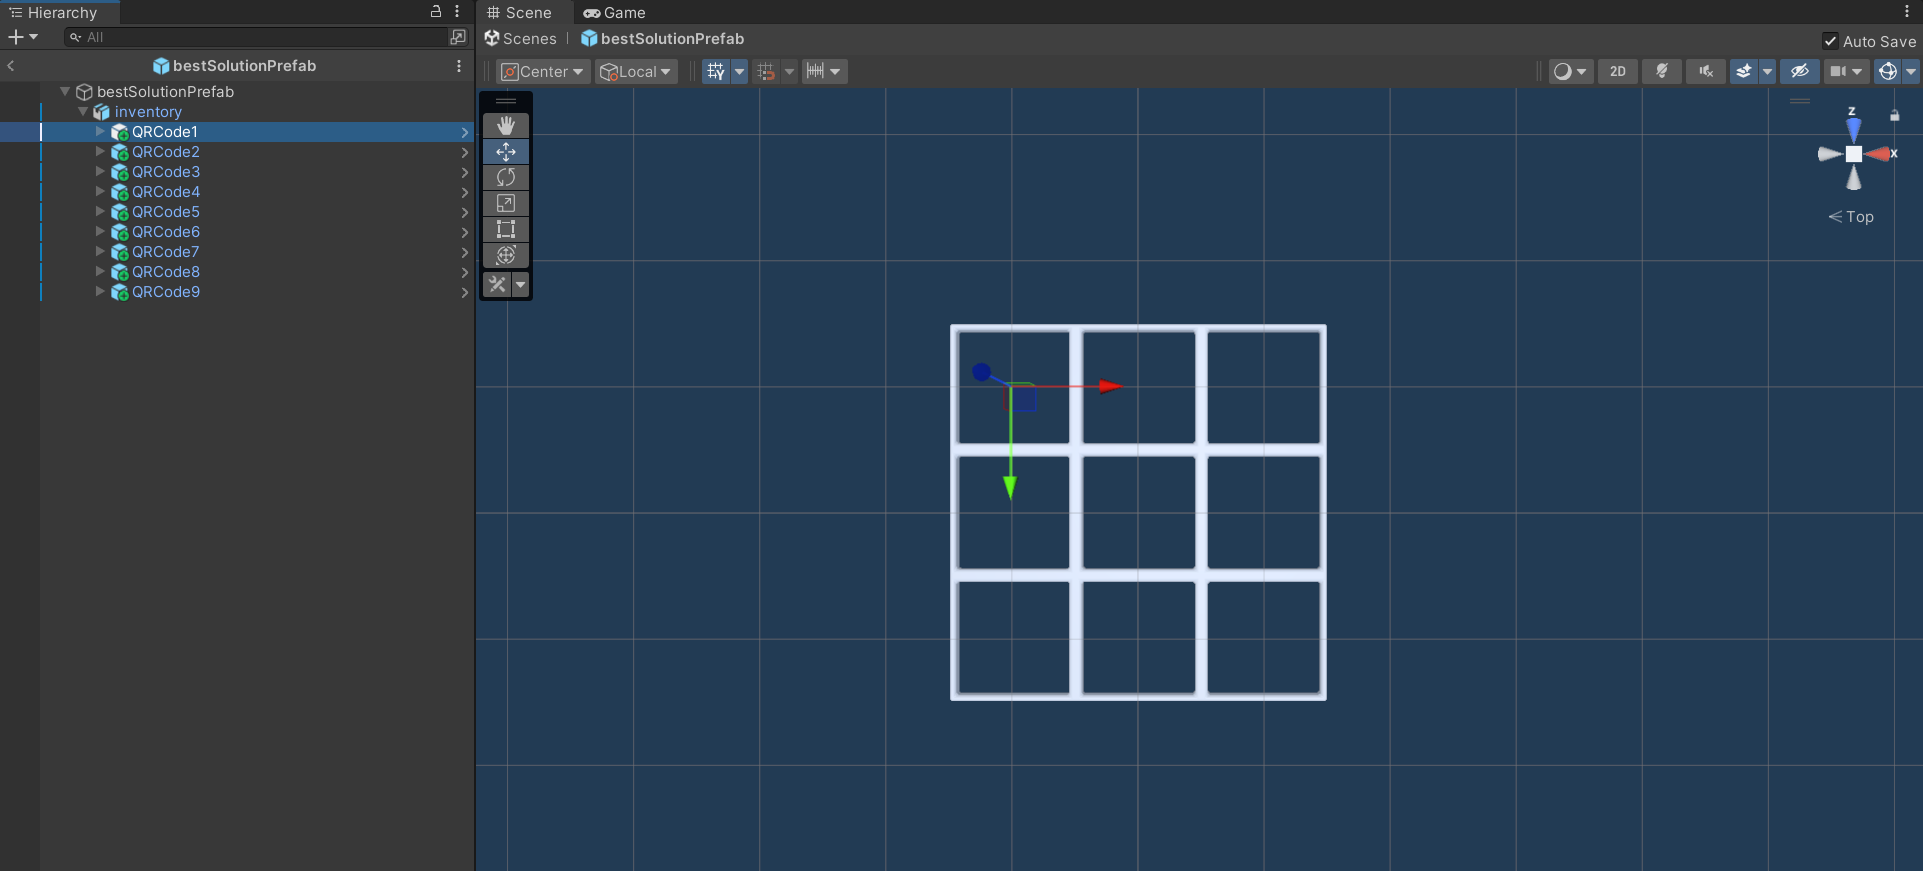
\includegraphics[scale=0.3]{images/prefShow}
    \caption{Inventar Prefab im Unity Editor}
    \label{fig:InvPrefUn}
\end{figure}
In dieser Abbildung ist zu erkennen, dass das \textit{QRItem1}-Prefab in der linken oberen Ecke (\textit{Index 0 des inventars})
positioniert ist. Des Weiteren sind alle \textit{QRItems} in den Zellen des Inventars angeordnet, um später anhand eines
Index das entsprechende Array zu durchlaufen, in dem die perfekte Lösung gespeichert ist. Auf diese Weise können die
zugehörigen Modelle in den entsprechenden \textit{QRItems} aktiviert und angezeigt werden.

\subsubsection{Script Aufruf}
Um die perfekte Lösung zu visualisieren, wird das \textit{PerfectSolutionVisualizer.cs}-Skript durch einen Knopfdruck
gestartet. Der zugehörige Knopf, der für das Auslösen dieses Skripts zuständig ist, befindet sich in dem Objekt
\textit{infoObject}. Der Aufruf dieses Skripts ist in der folgenden Abbildung \ref{fig:ScrAuf} dargestellt:
    \begin{figure}[H]
    \centering
    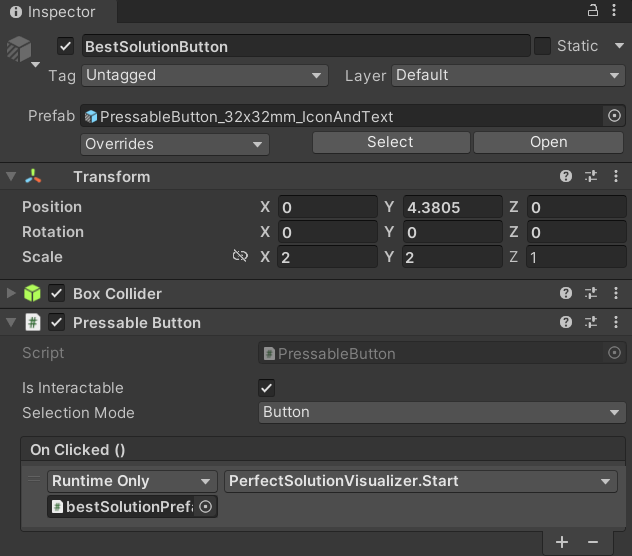
\includegraphics[scale=0.8]{images/perfSolBut}
    \caption{Script Aufruf bei Knopfdruck}
    \label{fig:ScrAuf}
\end{figure}
In dieser Abbildung sind die Komponenten des \textit{BestSolutionButton} zu sehen. Der zentrale Bestandteil dieser Abbildung
ist das Skript \textit{PressableButton}. Dieses Skript stellt die Funktion \textbf{OnClicked()} bereit, die einen einfachen
Knopfdruck implementiert. In dieser Funktion wird in diesem Fall die \textit{Start()}-Funktion des Skripts
\textit{PerfectSolutionVisualizer.cs} aufgerufen, um das Skript zu starten.

\subsubsection{PerfectSolutionVisualizer Klassenvariablen}
\begin{lstlisting}[style=csharp, caption={Klassenvariablen des PerfectSolutionVisualizer}, label=code:Klassenvariablen_PSV]
public GameObject inventoryObject;
public GameObject inventoryPlacementObject;
public GameObject KnapsackAlgoObject;
public Transform inventory;

private PlaceObjectOnLookedAtDesk anchorScript;
private KnapsackScript knapsackScript;
private Vector3 originalInventoryPosition;
private int[,] perfectSolution;
private bool isClicked = false;
private int numRows = 3;
private int numColumns = 3;
\end{lstlisting}\\
Die in Codeabschnitt \ref{code:Klassenvariablen_PSV} gezeigten Klassenvariablen gehören zu der \textit{PerfectSolutionVisualizer}
Klasse. Diese Variablen werden verwendet, um Objekte und Werte innerhalb des Unity Editors zu repräsentieren, die entweder
direkt festgelegt und übergeben werden oder von anderen Klassen aus Funktionalitätsgründen benötigt werden. Die
öffentlichen (\textit{public}) Variablen ermöglichen einen direkten Zugriff auf diese Objekte in der eigenen oder einer
anderen Klasse.

Besonders wichtig ist der Zugriff auf die Variablen \textit{inventoryPlacementObject} und \textit{KnapsackAlgoObject}, um
im weiteren Verlauf dieses Skripts auf die beiden angehängten Skripte dieser Game-Objekte zuzugreifen. Diese Skripte
speichern die Position des Inventars und das \textit{usedItems}-Array, die für das Anzeigen der perfekten Lösung benötigt
werden. Die Position des originalen Inventars ist notwendig, um die perfekte Lösung korrekt zu platzieren, während das
\textit{usedItems}-Array später benötigt wird, um das \textit{bestSolutionPrefab} anhand der gespeicherten Werte zu befüllen.

\subsubsection{Start des PerfectSolutionVisualizer}
Nachdem der \textit{BestSolutionButton} vom Benutzer gedrückt wurde, wird anschließend die \textbf{Start()} Funktion
aufgerufen, die den Prozess für das Anzeigen der perfekten Lösung startet. Der zugehörige Code lautet:
\begin{lstlisting}[style=csharp, caption={PerfectSolutionVisualizer Start}, label=code:Start_PSV]
public void Start()
{
    isClicked = !isClicked;
    if (isClicked == true)
    {
        anchorScript = inventoryPlacementObject.GetComponent<InventoryPlacementController>();
        originalInventoryPosition = anchorScript.objectPosition;
        knapsackSolver = KnapsackAlgoObject.GetComponent<KnapsackSolver>();
        perfectSolution = knapsackSolver.usedItems;
        printItems();
        setNewPosition();
        inventoryObject.SetActive(true);
        fillInventory();
    }
    else
    {
        inventoryObject.SetActive(false);
    }
}
\end{lstlisting}\\
Um sicherzustellen, dass der Benutzer die perfekte Lösung sowohl anzeigen (aktivieren) als auch wieder verstecken (deaktivieren)
kann, wird bei jedem Aufruf der \textbf{Start()} Funktion die boolsche Variable \textit{isClicked} negiert.

Wenn \textit{isClicked} den Wert \textit{true} hat, werden die \textit{objectPosition} der Klasse \textit{InventoryPlacementController}
und das \textit{usedItems}-Array der Klasse \textit{KnapsackSolver} gespeichert. Anschließend werden die Funktionen
\textbf{setNewPosition()} und \textbf{fillInventory()} aufgerufen, um die genaue Positionierung der perfekten Lösung und
das Befüllen des Inventars mit den entsprechenden Objekten zu gewährleisten.

Wenn \textit{isClicked} jedoch den Wert \textit{false} annimmt, wird das gesamte \textit{inventoryObject} durch die
Verwendung der \textbf{SetActive()} Funktion deaktiviert. Dadurch wird es unsichtbar für den Benutzer. Dies ermöglicht
eine einfache Handhabung der Anzeige und Ausblendung der perfekten Lösung.

\subsubsection{Setzen der neuen Position der perfekten Lösung}
Da die perfekte Lösung so positioniert werden muss, dass sie für den Benutzer leicht sichtbar ist, wird die folgende
Funktion aufgerufen:
\begin{lstlisting}[style=csharp, caption={Neue Position setzen}, label=code:newPos_PSV]
private void setNewPosition()
{
    Vector3 newPosition = originalInventoryPosition + Vector3.forward * 0.5f + Vector3.up * 0.205f;
    inventoryObject.transform.position = newPosition;
    Quaternion objectRotation = Quaternion.Euler(-45f, 0f, 0f);
    inventoryObject.transform.rotation = objectRotation;
}
\end{lstlisting}\\
Zunächst wird eine neue Position (\textit{newPosition}) für das Inventarobjekt berechnet. Diese Position basiert auf der
ursprünglichen Position des Inventarobjekts (\textit{originalInventoryPosition}). Die neue Position wird um 0,5 Einheiten
entlang der Vorwärtsachse (z-Achse) und um 0,205 Einheiten entlang der Aufwärtsachse (y-Achse) verschoben. Die Position
des Inventarobjekts wird auf die berechnete \textit{newPosition} gesetzt, wodurch das Objekt an die neue Position verschoben
wird. Anschließend wird eine Quaternion-Rotation (\textit{objectRotation}) erstellt, um das Inventarobjekt um -45 Grad
entlang der x-Achse zu kippen. Schließlich wird die Rotation des Inventarobjekts auf die berechnete \texttt{objectRotation}
gesetzt, um das Objekt entsprechend zu kippen.

\subsubsection{Perfekte Lösung füllen}
Aufgrund dessen, dass das zuvor platzierte Objekt lediglich ein leeres Raster darstellt, ist es erforderlich, dieses
Raster anschließend mit den entsprechenden Elementen zu füllen, um die perfekte Lösung zu repräsentieren. Zu diesem Zweck
wird im weiteren Verlauf die Funktion \textbf{fillInventory()} aufgerufen. Der Code dieser Funktion:
\begin{lstlisting}[style=csharp, caption={Inventar füllen}, label=code:invFül_PSV]
private void fillInventory()
{
    for (int i = 0; i < numRows; i++)
    {
        for (int j = 0; j < numColumns; j++)
        {
            int id = perfectSolution[i, j];
            if (perfectSolution[i, j] == 0)
                continue;
            else
            {
                string qrCodeName = "QRCode" + (i * numColumns + j + 1);
                Transform qrCodeTransform = inventory.Find(qrCodeName);
                if (qrCodeTransform != null)
                {
                    Transform childTransform = qrCodeTransform.Find(id.ToString());
                    if (childTransform != null)
                    {
                        childTransform.gameObject.SetActive(true);
                    }
                }
                else
                {
                    Debug.LogError($"QRCode {qrCodeName} not found in the inventory");
                }
            }
        }
    }
}
\end{lstlisting}\\
Die vorliegende Funktion durchläuft das zweidimensionale Array \textit{perfectSolution}, das die perfekte Lösung repräsentiert.
Zu Beginn wird die ID an der Stelle $[i, j]$ des Arrays gespeichert. An jeder Position wird zunächst überprüft, ob die
gespeicherte ID gleich 0 ist. In diesem Fall wird der Schleifendurchlauf mit \textit{continue} übersprungen, da der Wert
0 darauf hinweist, dass an dieser Stelle kein Item liegt.

Wenn der Wert an der Stelle $[i, j]$ größer als 0 ist, deutet dies darauf hin, dass an dieser Position im Inventar ein
konkretes Element vorliegt. Zur Identifizierung dieses Elements und zum Auffinden des entsprechenden QRItems wird ein
stringbasierter Bezeichner \textit{qrCodeName} generiert. Dieser Bezeichner wird durch die Konkatenation des Präfixes
\textit{QRCode} mit dem Ergebnis der Berechnung $i \times \text{numColumns} + j + 1$ erzeugt. Diese Berechnung berücksichtigt
die aktuelle Position im zweidimensionalen Array und ermöglicht die Erstellung eines eindeutigen Bezeichners für das QRItem.
Auf diese Weise wird das QRItem erfolgreich identifiziert und kann anschließend im Inventar lokalisiert werden.\\
\\
Um diesen Vorgang der Identifikation des korrekten \textit{QRItem} Prefabs besser zu veranschaulichen wird hierfür ein
Beispiel herangezogen, dass die Berechcnung anhand von Testwerten durchführt.

\begin{quote}
Angenommen in der Schleife hat \textbf{i} den Wert 1 und \textbf{j} den Wert 1. Dies bedeutet, dass das Array momentan
an der Stelle $[1, 1]$ steht. Das \texttt{bestSolutionPrefab} ist so strukturiert, dass der Index nicht mit 0, sondern
mit 1 beginnt. Daher wird in der Berechnung am Ende $+ 1$ hinzugefügt, um dies zu berücksichtigen. Somit wird an der
Stelle $[i, j]$ das \textit{QRItem5} dem Array zugeordnet.
\end{quote}

Nachdem das richtige \textit{QRItem} identifiziert wurde, wird anschließend das dem Inventar-Objekt untergeordnete
\textit{QRItem} Prefab mit diesem Namen gespeichert. Wenn dieses Objekt ungleich null ist, wird von diesem Prefab das
untergeordnete Modell anhand der zuvor gespeicherten \textit{ID} aktiviert, um es in dem Inventar-Raster anzuzeigen.
Andernfalls wird eine Fehlermeldung in die \textit{Logdatei} geschrieben. Der Zustand nach dem Abschluss dieser Funktion
ist in der folgenden Abbildung \ref{fig:perfSolUserPOV} zu sehen.
\begin{figure}[H]
    \centering
    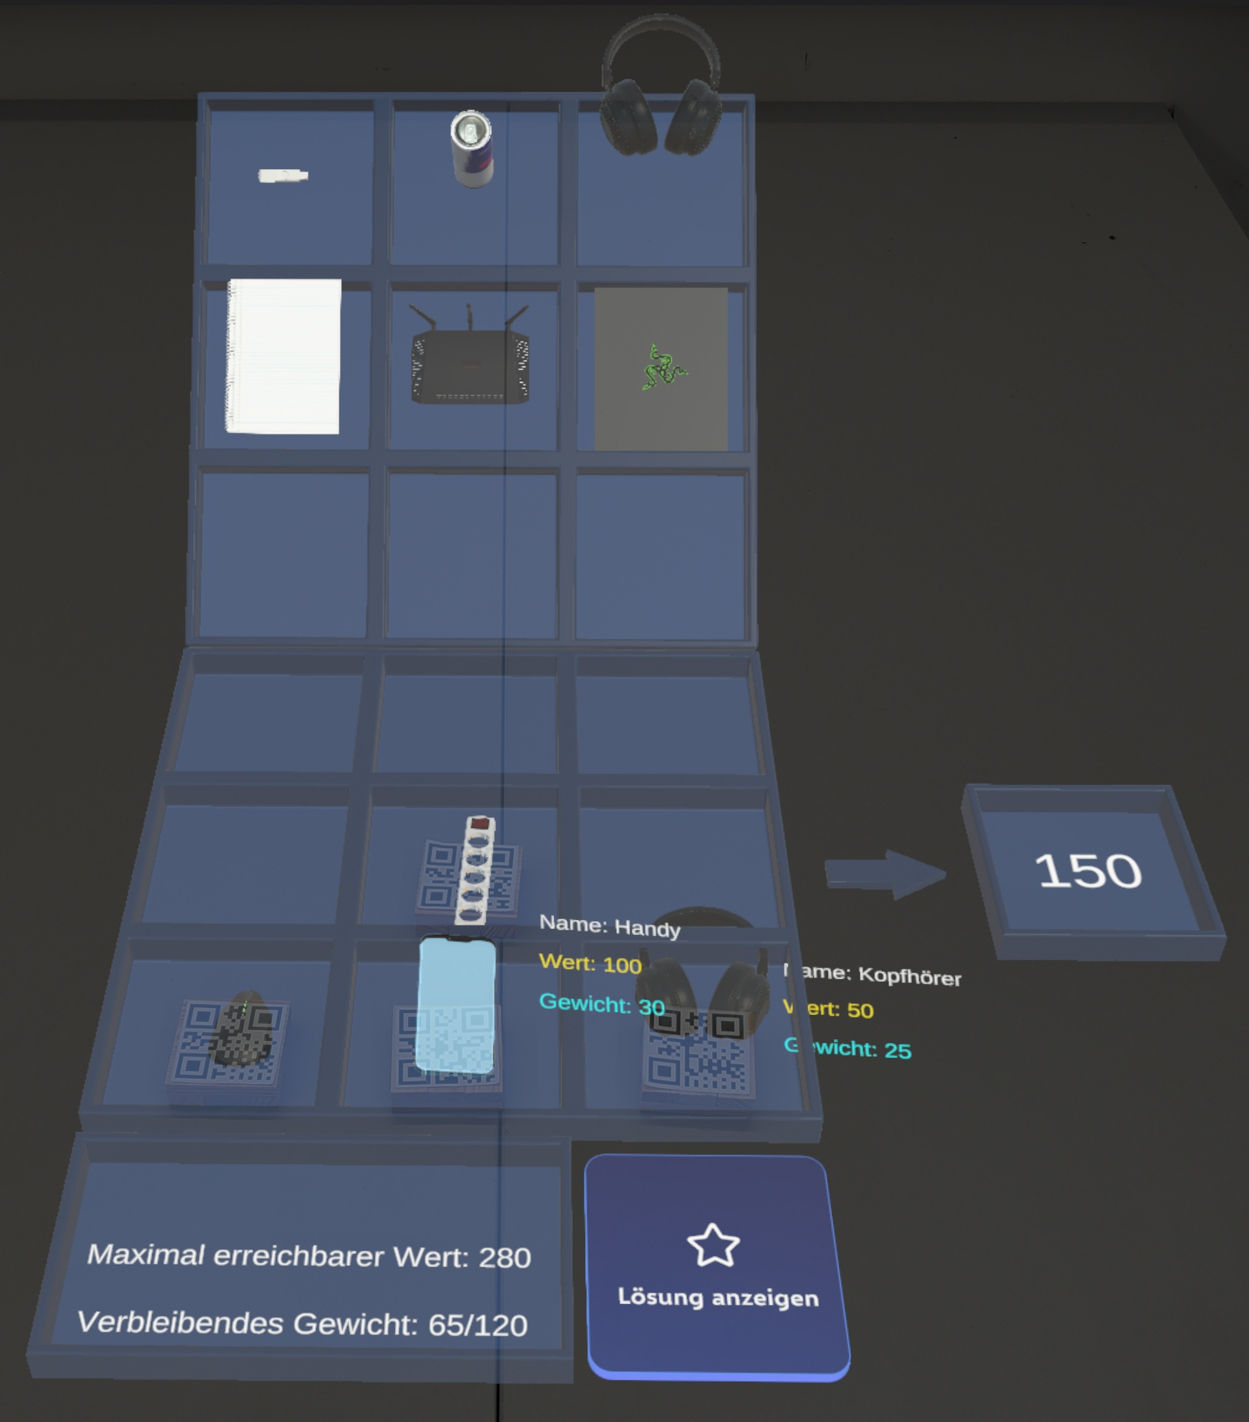
\includegraphics[scale=0.8]{images/perfSolUserPOV}
    \caption{Perfekte Lösung}
    \label{fig:perfSolUserPOV}
\end{figure}

\section{Performance und Qualtitätssicherung} \marginpar{\small\(\rightarrow\) HAYLAZ}
\subsection{Unit-Tests}
Unit-Tests sind ein wichtiger Bestandteil der Qualitätssicherung. Sie ermöglichen die Überprüfung der korrekten
Funktionalität einzelner Komponenten und stellen sicher, dass sie wie erwartet arbeiten. Im Rahmen dieses Projekts wurden
Unit-Tests verwendet, um den Knapsack-Algorithmus zu überprüfen.  Die Tests wurden mithilfe des Unity Test Frameworks
erstellt und ausgeführt. Dieses Tool wurde speziell für die Erstellung und Ausführung von Unit-Tests in Unity entwickelt.
Durch die sorgfältige Gestaltung der Tests wurde sichergestellt, dass der Algorithmus nicht nur die erwarteten Ergebnisse
zurückgibt, sondern auch die vorgegebene Laufzeit einhält. Die Tests wurden innerhalb der Entwicklungsumgebung von Unity
durchgeführt. Die Ergebnisse wurden genau überwacht, um sicherzustellen, dass der Algorithmus zuverlässig funktioniert.

\subsection{Unity Test Framework}
Das Unity Test Framework bietet eine breite Palette von Funktionen, mit denen Entwickler umfassende Tests für ihre
Unity-Skripte schreiben und ausführen können. Dabei können verschiedene Aspekte der Skripte auf ihre korrekte Funktionalität
überprüft werden. Dazu gehören das Testen von Variablen, das Aufrufen von Funktionen und das Überprüfen von erwarteten
Ergebnissen. Entwickler können dank dieser umfangreichen Funktionen sicherstellen, dass ihre Unity-Anwendungen robust
und zuverlässig sind. So schaffen sie eine solide Grundlage für die Qualitätssicherung.

\subsection{Performance-Messung}
Die Performance des Knapsack-Algorithmus wurde mithilfe von Unit-Tests überprüft. Dabei wurde die Laufzeit des Algorithmus
für verschiedene Eingabegrößen gemessen. Die Ergebnisse wurden sorgfältig analysiert, um sicherzustellen, dass der Algorithmus
die erwartete Laufzeit einhält. Es wurden verschiedene Algorithmen und Implementierungen getestet, um die optimale
Leistung zu erzielen. Die Ergebnisse der Performance-Messung wurden genau überwacht, um sicherzustellen, dass der
Algorithmus zuverlässig und effizient arbeitet.

\begin{lstlisting}[style=csharp, caption={Unit Test Klasse}, label=code:UnitTest]
public class AlgoTest
{
GameObject testObject;
KnapsackScript knapsackScript;
int[,] usedItems;
int capacity = 120;
...
\end{lstlisting}\\

Dies ist eine Testklasse in C#, welche den Knapsack-Algorithmus implementiert und testet.

Die Klasse AlgoTest enthält Testfunktionen für zwei verschiedene Knapsack-Algorithmen.

Es werden mehrere Variablen definiert, darunter ein testObject, das zu testende knapsackScript und capacity, die maximale
Größe des Rucksacks, die für die Tests benötigt wird. Die Methoden SetUp und TearDown sind mit den Attributen [SetUp] und
[TearDown] versehen. Diese Attribute werden vom Framework erkannt und dienen dazu, nach jedem Test die Umgebung zu reinigen
und neu aufzusetzen.Es wird eine Instanz des KnapsackScript erstellt und wieder zerstört, um sicherzustellen, dass die
Tests in einer sauberen Umgebung ausgeführt werden.
\newpage

\begin{lstlisting}[style=csharp, caption={Unit Test Methode}, label=code:Test Methode]
// Ein Test verhält sich wie eine normale Methode
[Test]
public void KnapsackMaxValue_ReturnsCorrectValue()
{
    // Gibt eine Menge von Gegenständen für den Rucksack an
    Dictionary<int, QRData> items = new Dictionary<int, QRData>() {
    {1, new QRData { id = 1, weight = 50, value = 100 }},
    ... //weitere Testobjekte

    System.Random random = new System.Random();
    for (int i = 11; i <= 100; i++)
    {
        int randomWeight = random.Next(1, 51);
        int randomValue = random.Next(1, 101);

        items.Add(i, new QRData { id = i, weight = randomWeight, value = randomValue });
    }
\end{lstlisting}\\

Der Unit-Test \texttt{KnapsackMaxValue\_ReturnsCorrectValue} testet die Methode \texttt{KnapsackMaxValue} des \texttt{KnapsackScript}.
Es werden verschiedene Gegenstände in dem Dictionary definiert. Außerdem werden noch weitere Items mit zufälligen Werten
in das Dictionary hinzugefügt, damit auch getestet wird, ob der Algorithmus konsistent richtige Lösungen liefert.

\begin{lstlisting}[style=csharp, caption={Zeitmessung}, label=code:Zeitmessung]
// Messung der Ausführungszeit für KnapsackMaxValue
System.Diagnostics.Stopwatch knapsackMaxValueStopwatch = System.Diagnostics.Stopwatch.StartNew();
int maxValue = knapsackScript.KnapsackMaxValue(out usedItems);
knapsackMaxValueStopwatch.Stop();
Debug.Log($"Die Ausführungszeit von KnapsackMaxValue beträgt: {knapsackMaxValueStopwatch.ElapsedMilliseconds} ms");

// Messung der Ausführungszeit für KnapsackMaxValueRecursive
System.Diagnostics.Stopwatch recursiveStopwatch = System.Diagnostics.Stopwatch.StartNew();
int maxValueComp = KnapsackMaxValueRecursive(items.Count, capacity, items, new Dictionary<(int, int), int>());
recursiveStopwatch.Stop();
Debug.Log($"Die Ausführungszeit von KnapsackMaxValueRecursive beträgt: {recursiveStopwatch.ElapsedMilliseconds} ms");

// Überprüfen, ob die Werte übereinstimmen
Assert.AreEqual(maxValueComp, maxValue);
\end{lstlisting}\\

Anschließend wird die Ausführungszeit sowohl der iterativen (\texttt{KnapsackMaxValue}) als auch der rekursiven
(\texttt{KnapsackMaxValueRecursive}) Implementierung des Knapsack-Algorithmus gemessen. Schließlich wird überprüft,
ob beide Implementierungen denselben Wert zurückgeben.

\newpage

\begin{lstlisting}[style=csharp, caption={Rekursiver Algorithmus}, label=code:Rekursiver Algorithmus]
// Rekursive Implementierung des Knapsack-Algorithmus zur Berechnung des maximalen Werts
public int KnapsackMaxValueRecursive(int n, int remainingCapacity, Dictionary<int, QRData> items, Dictionary<(int, int), int> memo)
{
    if (n == 0 || remainingCapacity == 0)
    return 0;

    if (memo.TryGetValue((n, remainingCapacity), out int memoizedValue))
    return memoizedValue;

    if (items[n].weight > remainingCapacity)
    {
    memo[(n, remainingCapacity)] = KnapsackMaxValueRecursive(n - 1, remainingCapacity, items, memo);
    return memo[(n, remainingCapacity)];
    }

    int includedValue = items[n].value + KnapsackMaxValueRecursive(n - 1, remainingCapacity - items[n].weight, items, memo);
    int excludedValue = KnapsackMaxValueRecursive(n - 1, remainingCapacity, items, memo);

    int result = Math.Max(includedValue, excludedValue);

    memo[(n, remainingCapacity)] = result;

    return result;
}
\end{lstlisting}\\

Die Methode \texttt{KnapsackMaxValueRecursive} ist eine rekursive Implementierung des Knapsack-Algorithmus. Der maximale Wert, den
der Rucksack aufnehmen kann, wird berechnet, indem die Elemente rekursiv entweder eingeschlossen oder ausgeschlossen werden.
Es wurde darauf geachtet, verschiedene Implementierungen zu testen, um sicherzustellen, dass die optimale Implementierung verwendet wird.
%TODO Grafik der Testergebnisse und Unterschiede der Laufzeiten von rekursiver und iterativer Implementierung erklären

Die Testmethode \texttt{KnapsackMaxValue\_ReturnsCorrectValue} wird für jede Konfiguration von Gegenständen im Rucksack ausgeführt,
um sicherzustellen, dass die Implementierung des Knapsack-Algorithmus korrekt funktioniert.

Dabei wird die rekursive Implementierung \texttt{KnapsackMaxValueRecursive} als Vergleich verwendet, um sicherzustellen, dass
auch die iterative Implementierung \texttt{KnapsackMaxValue} korrekt ist.

%Performance-Messung
